% Options for packages loaded elsewhere
\PassOptionsToPackage{unicode}{hyperref}
\PassOptionsToPackage{hyphens}{url}
%
\documentclass[
]{book}
\usepackage{amsmath,amssymb}
\usepackage{iftex}
\ifPDFTeX
  \usepackage[T1]{fontenc}
  \usepackage[utf8]{inputenc}
  \usepackage{textcomp} % provide euro and other symbols
\else % if luatex or xetex
  \usepackage{unicode-math} % this also loads fontspec
  \defaultfontfeatures{Scale=MatchLowercase}
  \defaultfontfeatures[\rmfamily]{Ligatures=TeX,Scale=1}
\fi
\usepackage{lmodern}
\ifPDFTeX\else
  % xetex/luatex font selection
\fi
% Use upquote if available, for straight quotes in verbatim environments
\IfFileExists{upquote.sty}{\usepackage{upquote}}{}
\IfFileExists{microtype.sty}{% use microtype if available
  \usepackage[]{microtype}
  \UseMicrotypeSet[protrusion]{basicmath} % disable protrusion for tt fonts
}{}
\makeatletter
\@ifundefined{KOMAClassName}{% if non-KOMA class
  \IfFileExists{parskip.sty}{%
    \usepackage{parskip}
  }{% else
    \setlength{\parindent}{0pt}
    \setlength{\parskip}{6pt plus 2pt minus 1pt}}
}{% if KOMA class
  \KOMAoptions{parskip=half}}
\makeatother
\usepackage{xcolor}
\usepackage{color}
\usepackage{fancyvrb}
\newcommand{\VerbBar}{|}
\newcommand{\VERB}{\Verb[commandchars=\\\{\}]}
\DefineVerbatimEnvironment{Highlighting}{Verbatim}{commandchars=\\\{\}}
% Add ',fontsize=\small' for more characters per line
\usepackage{framed}
\definecolor{shadecolor}{RGB}{248,248,248}
\newenvironment{Shaded}{\begin{snugshade}}{\end{snugshade}}
\newcommand{\AlertTok}[1]{\textcolor[rgb]{0.94,0.16,0.16}{#1}}
\newcommand{\AnnotationTok}[1]{\textcolor[rgb]{0.56,0.35,0.01}{\textbf{\textit{#1}}}}
\newcommand{\AttributeTok}[1]{\textcolor[rgb]{0.13,0.29,0.53}{#1}}
\newcommand{\BaseNTok}[1]{\textcolor[rgb]{0.00,0.00,0.81}{#1}}
\newcommand{\BuiltInTok}[1]{#1}
\newcommand{\CharTok}[1]{\textcolor[rgb]{0.31,0.60,0.02}{#1}}
\newcommand{\CommentTok}[1]{\textcolor[rgb]{0.56,0.35,0.01}{\textit{#1}}}
\newcommand{\CommentVarTok}[1]{\textcolor[rgb]{0.56,0.35,0.01}{\textbf{\textit{#1}}}}
\newcommand{\ConstantTok}[1]{\textcolor[rgb]{0.56,0.35,0.01}{#1}}
\newcommand{\ControlFlowTok}[1]{\textcolor[rgb]{0.13,0.29,0.53}{\textbf{#1}}}
\newcommand{\DataTypeTok}[1]{\textcolor[rgb]{0.13,0.29,0.53}{#1}}
\newcommand{\DecValTok}[1]{\textcolor[rgb]{0.00,0.00,0.81}{#1}}
\newcommand{\DocumentationTok}[1]{\textcolor[rgb]{0.56,0.35,0.01}{\textbf{\textit{#1}}}}
\newcommand{\ErrorTok}[1]{\textcolor[rgb]{0.64,0.00,0.00}{\textbf{#1}}}
\newcommand{\ExtensionTok}[1]{#1}
\newcommand{\FloatTok}[1]{\textcolor[rgb]{0.00,0.00,0.81}{#1}}
\newcommand{\FunctionTok}[1]{\textcolor[rgb]{0.13,0.29,0.53}{\textbf{#1}}}
\newcommand{\ImportTok}[1]{#1}
\newcommand{\InformationTok}[1]{\textcolor[rgb]{0.56,0.35,0.01}{\textbf{\textit{#1}}}}
\newcommand{\KeywordTok}[1]{\textcolor[rgb]{0.13,0.29,0.53}{\textbf{#1}}}
\newcommand{\NormalTok}[1]{#1}
\newcommand{\OperatorTok}[1]{\textcolor[rgb]{0.81,0.36,0.00}{\textbf{#1}}}
\newcommand{\OtherTok}[1]{\textcolor[rgb]{0.56,0.35,0.01}{#1}}
\newcommand{\PreprocessorTok}[1]{\textcolor[rgb]{0.56,0.35,0.01}{\textit{#1}}}
\newcommand{\RegionMarkerTok}[1]{#1}
\newcommand{\SpecialCharTok}[1]{\textcolor[rgb]{0.81,0.36,0.00}{\textbf{#1}}}
\newcommand{\SpecialStringTok}[1]{\textcolor[rgb]{0.31,0.60,0.02}{#1}}
\newcommand{\StringTok}[1]{\textcolor[rgb]{0.31,0.60,0.02}{#1}}
\newcommand{\VariableTok}[1]{\textcolor[rgb]{0.00,0.00,0.00}{#1}}
\newcommand{\VerbatimStringTok}[1]{\textcolor[rgb]{0.31,0.60,0.02}{#1}}
\newcommand{\WarningTok}[1]{\textcolor[rgb]{0.56,0.35,0.01}{\textbf{\textit{#1}}}}
\usepackage{longtable,booktabs,array}
\usepackage{calc} % for calculating minipage widths
% Correct order of tables after \paragraph or \subparagraph
\usepackage{etoolbox}
\makeatletter
\patchcmd\longtable{\par}{\if@noskipsec\mbox{}\fi\par}{}{}
\makeatother
% Allow footnotes in longtable head/foot
\IfFileExists{footnotehyper.sty}{\usepackage{footnotehyper}}{\usepackage{footnote}}
\makesavenoteenv{longtable}
\usepackage{graphicx}
\makeatletter
\def\maxwidth{\ifdim\Gin@nat@width>\linewidth\linewidth\else\Gin@nat@width\fi}
\def\maxheight{\ifdim\Gin@nat@height>\textheight\textheight\else\Gin@nat@height\fi}
\makeatother
% Scale images if necessary, so that they will not overflow the page
% margins by default, and it is still possible to overwrite the defaults
% using explicit options in \includegraphics[width, height, ...]{}
\setkeys{Gin}{width=\maxwidth,height=\maxheight,keepaspectratio}
% Set default figure placement to htbp
\makeatletter
\def\fps@figure{htbp}
\makeatother
\setlength{\emergencystretch}{3em} % prevent overfull lines
\providecommand{\tightlist}{%
  \setlength{\itemsep}{0pt}\setlength{\parskip}{0pt}}
\setcounter{secnumdepth}{5}
\usepackage{booktabs}
\usepackage{booktabs}
\usepackage{caption}
\usepackage{longtable}
\usepackage{colortbl}
\usepackage{array}
\usepackage{float}
\usepackage{tabularray}
\usepackage[normalem]{ulem}
\usepackage{graphicx}
\UseTblrLibrary{booktabs}
\UseTblrLibrary{siunitx}
\NewTableCommand{\tinytableDefineColor}[3]{\definecolor{#1}{#2}{#3}}
\newcommand{\tinytableTabularrayUnderline}[1]{\underline{#1}}
\newcommand{\tinytableTabularrayStrikeout}[1]{\sout{#1}}
\ifLuaTeX
  \usepackage{selnolig}  % disable illegal ligatures
\fi
\usepackage[]{natbib}
\bibliographystyle{plainnat}
\IfFileExists{bookmark.sty}{\usepackage{bookmark}}{\usepackage{hyperref}}
\IfFileExists{xurl.sty}{\usepackage{xurl}}{} % add URL line breaks if available
\urlstyle{same}
\hypersetup{
  pdftitle={西山ほか(2019)『計量経済学』有斐閣の練習問題解答とRでの再現},
  pdfauthor={石井 俊輔},
  hidelinks,
  pdfcreator={LaTeX via pandoc}}

\title{西山ほか(2019)『計量経済学』有斐閣の練習問題解答とRでの再現}
\author{石井 俊輔}
\date{2024-05-02}

\begin{document}
\maketitle

{
\setcounter{tocdepth}{1}
\tableofcontents
}
\hypertarget{ux306fux3058ux3081ux306b}{%
\chapter*{はじめに}\label{ux306fux3058ux3081ux306b}}
\addcontentsline{toc}{chapter}{はじめに}

西山ほか(2019)『計量経済学』有斐閣 (\href{https://www.yuhikaku.co.jp/books/detail/9784641053854}{出版社リンク}) の練習問題解答とRでの再現です.
サイト: \url{https://sishii0418.github.io/nishiyama_econometrics/}

必要なRパッケージをインストール:

\begin{Shaded}
\begin{Highlighting}[]
\FunctionTok{install.packages}\NormalTok{(}\StringTok{"tidyverse"}\NormalTok{)}
\FunctionTok{install.packages}\NormalTok{(}\StringTok{"openxlsx"}\NormalTok{)}
\FunctionTok{install.packages}\NormalTok{(}\StringTok{"haven"}\NormalTok{)}
\FunctionTok{install.packages}\NormalTok{(}\StringTok{"wooldridge"}\NormalTok{)}
\FunctionTok{install.packages}\NormalTok{(}\StringTok{"fixest"}\NormalTok{)}
\FunctionTok{install.packages}\NormalTok{(}\StringTok{"car"}\NormalTok{)}
\FunctionTok{install.packages}\NormalTok{(}\StringTok{"knitr"}\NormalTok{)}
\FunctionTok{install.packages}\NormalTok{(}\StringTok{"modelsummary"}\NormalTok{)}
\FunctionTok{install.packages}\NormalTok{(}\StringTok{"estimatr"}\NormalTok{)}
\end{Highlighting}
\end{Shaded}

\hypertarget{ux65b9ux91dd}{%
\section*{方針}\label{ux65b9ux91dd}}
\addcontentsline{toc}{section}{方針}

\begin{itemize}
\tightlist
\item
  不均一分散に頑健な回帰分析は\texttt{estimatr::lm\_robust()}を使っています.
\item
  回帰結果の表は\texttt{modelsummary}, その他の表は\texttt{gt}などを使い, 容易にHTML, LaTeX間で変換ができるようにしています.
\item
  \texttt{tidyverse}を使い, 図は\texttt{ggplot2}で出力しています.
\end{itemize}

\hypertarget{ux4f3cux305fux3088ux3046ux306aux30b5ux30a4ux30c8}{%
\section*{似たようなサイト}\label{ux4f3cux305fux3088ux3046ux306aux30b5ux30a4ux30c8}}
\addcontentsline{toc}{section}{似たようなサイト}

公式の解答はないようですが, ほかに似たようなサイトとして以下があります (ほかにもご存知でしたらご教授ください).

\begin{itemize}
\tightlist
\item
  北川梨津 (2020) 『西山 他『計量経済学』のためのR』(\url{https://ritsu1997.github.io/r-for-nlas-econometrics/})\footnote{勝手ながら, だいぶ参考にさせていただきました.}.
\item
  @kpd0605(ビル・エヴァンス ギャンビット) (2024) 『『計量経済学』(有斐閣)実践問題解答例(順次追加)』(\url{https://qiita.com/kpd0605/items/28ca24fe8b192612e67c}).
\end{itemize}

\hypertarget{ch2}{%
\chapter*{第2章 データの整理と確率変数の基礎}\label{ch2}}
\addcontentsline{toc}{chapter}{第2章 データの整理と確率変数の基礎}

先に\href{https://www.yuhikaku.co.jp/books/detail/9784641053854}{出版社サイト}よりデータをダウンロードする.

\begin{Shaded}
\begin{Highlighting}[]
\CommentTok{\# サポートファイルへのリンク}
\NormalTok{curl }\OtherTok{\textless{}{-}} \StringTok{"https://www.yuhikaku.co.jp/static\_files/05385\_support02.zip"}
\CommentTok{\# ダウンロード保存用フォルダが存在しない場合, 作成}
\ControlFlowTok{if}\NormalTok{(}\SpecialCharTok{!}\FunctionTok{dir.exists}\NormalTok{(}\StringTok{"downloads"}\NormalTok{))\{}
    \FunctionTok{dir.create}\NormalTok{(}\StringTok{"downloads"}\NormalTok{)}
\NormalTok{\}}
\NormalTok{cdestfile }\OtherTok{\textless{}{-}} \StringTok{"downloads/support02.zip"}
\FunctionTok{download.file}\NormalTok{(curl, cdestfile)}
\CommentTok{\# データ保存用フォルダが存在しない場合, 作成}
\ControlFlowTok{if}\NormalTok{(}\SpecialCharTok{!}\FunctionTok{dir.exists}\NormalTok{(}\StringTok{"data"}\NormalTok{))\{}
    \FunctionTok{dir.create}\NormalTok{(}\StringTok{"data"}\NormalTok{)}
\NormalTok{\}}
\CommentTok{\# WSL上のRで解凍すると文字化けするので、Linuxのコマンドを外部呼び出し}
\CommentTok{\# Windowsの場合は別途コマンドを用いる.}
\ControlFlowTok{if}\NormalTok{(.Platform}\SpecialCharTok{$}\NormalTok{OS.type }\SpecialCharTok{==} \StringTok{"unix"}\NormalTok{) \{}
    \FunctionTok{system}\NormalTok{(}\FunctionTok{sprintf}\NormalTok{(}\StringTok{\textquotesingle{}unzip {-}n {-}Ocp932 \%s {-}d \%s\textquotesingle{}}\NormalTok{, }\StringTok{"downloads/support02.zip"}\NormalTok{, }\StringTok{"./data"}\NormalTok{))}
\NormalTok{\} }\ControlFlowTok{else}\NormalTok{ \{}
    \FunctionTok{print}\NormalTok{(}\StringTok{"Windowsで解凍するコマンドを別途追加せよ."}\NormalTok{)}
\NormalTok{\}}
\end{Highlighting}
\end{Shaded}

必要なライブラリを読み込む.

\begin{Shaded}
\begin{Highlighting}[]
\FunctionTok{library}\NormalTok{(tidyverse)}
\DocumentationTok{\#\# {-}{-} Attaching core tidyverse packages {-}{-}{-}{-}{-}{-}{-}{-}{-}{-}{-}{-}{-}{-}{-}{-}{-}{-}{-}{-}{-}{-}{-}{-} tidyverse 2.0.0 {-}{-}}
\DocumentationTok{\#\# v dplyr     1.1.4     v readr     2.1.5}
\DocumentationTok{\#\# v forcats   1.0.0     v stringr   1.5.1}
\DocumentationTok{\#\# v ggplot2   3.5.0     v tibble    3.2.1}
\DocumentationTok{\#\# v lubridate 1.9.3     v tidyr     1.3.1}
\DocumentationTok{\#\# v purrr     1.0.2     }
\DocumentationTok{\#\# {-}{-} Conflicts {-}{-}{-}{-}{-}{-}{-}{-}{-}{-}{-}{-}{-}{-}{-}{-}{-}{-}{-}{-}{-}{-}{-}{-}{-}{-}{-}{-}{-}{-}{-}{-}{-}{-}{-}{-}{-}{-}{-}{-}{-}{-} tidyverse\_conflicts() {-}{-}}
\DocumentationTok{\#\# x dplyr::filter() masks stats::filter()}
\DocumentationTok{\#\# x dplyr::lag()    masks stats::lag()}
\DocumentationTok{\#\# i Use the conflicted package (\textless{}http://conflicted.r{-}lib.org/\textgreater{}) to force all conflicts to become errors}
\end{Highlighting}
\end{Shaded}

\hypertarget{ux7df4ux7fd2ux554fux984c-2-1-ux78baux8a8d}{%
\section*{練習問題 2-1 {[}確認{]}}\label{ux7df4ux7fd2ux554fux984c-2-1-ux78baux8a8d}}
\addcontentsline{toc}{section}{練習問題 2-1 {[}確認{]}}

R には最頻値を求める関数がないようなので, 別途関数\texttt{Mode()}を定義する.

\begin{Shaded}
\begin{Highlighting}[]
\NormalTok{data21 }\OtherTok{\textless{}{-}} \FunctionTok{read.table}\NormalTok{(}\StringTok{"data/02\_第2章/02\_practice\_01.csv"}\NormalTok{)}

\FunctionTok{mean}\NormalTok{(data21}\SpecialCharTok{$}\NormalTok{V1)}
\DocumentationTok{\#\# [1] 10}
\FunctionTok{var}\NormalTok{(data21}\SpecialCharTok{$}\NormalTok{V1)}
\DocumentationTok{\#\# [1] 18.10526}
\FunctionTok{median}\NormalTok{(data21}\SpecialCharTok{$}\NormalTok{V1)}
\DocumentationTok{\#\# [1] 10}

\NormalTok{Mode }\OtherTok{\textless{}{-}} \ControlFlowTok{function}\NormalTok{(x) \{}
\NormalTok{    ux }\OtherTok{\textless{}{-}} \FunctionTok{unique}\NormalTok{(x)}
\NormalTok{    tab }\OtherTok{\textless{}{-}} \FunctionTok{tabulate}\NormalTok{(}\FunctionTok{match}\NormalTok{(x, ux))}
\NormalTok{    ux[tab }\SpecialCharTok{==} \FunctionTok{max}\NormalTok{(tab)]}
\NormalTok{\}}

\FunctionTok{Mode}\NormalTok{(data21}\SpecialCharTok{$}\NormalTok{V1)}
\DocumentationTok{\#\# [1] 10}
\end{Highlighting}
\end{Shaded}

\hypertarget{ux7df4ux7fd2ux554fux984c-2-3-ux78baux8a8d}{%
\section*{練習問題 2-3 {[}確認{]}}\label{ux7df4ux7fd2ux554fux984c-2-3-ux78baux8a8d}}
\addcontentsline{toc}{section}{練習問題 2-3 {[}確認{]}}

\begin{Shaded}
\begin{Highlighting}[]
\NormalTok{data23 }\OtherTok{\textless{}{-}} \FunctionTok{read.table}\NormalTok{(}\StringTok{"data/02\_第2章/02\_practice\_03.csv"}\NormalTok{, }\AttributeTok{sep=}\StringTok{","}\NormalTok{)}

\NormalTok{x }\OtherTok{\textless{}{-}}\NormalTok{ data23}\SpecialCharTok{$}\NormalTok{V1}
\NormalTok{y }\OtherTok{\textless{}{-}}\NormalTok{ data23}\SpecialCharTok{$}\NormalTok{V2}

\NormalTok{data23 }\SpecialCharTok{\%\textgreater{}\%}
    \FunctionTok{ggplot}\NormalTok{(}\FunctionTok{aes}\NormalTok{(}\AttributeTok{x =}\NormalTok{ x, }\AttributeTok{y =}\NormalTok{ y)) }\SpecialCharTok{+}
    \FunctionTok{geom\_point}\NormalTok{()}
\end{Highlighting}
\end{Shaded}

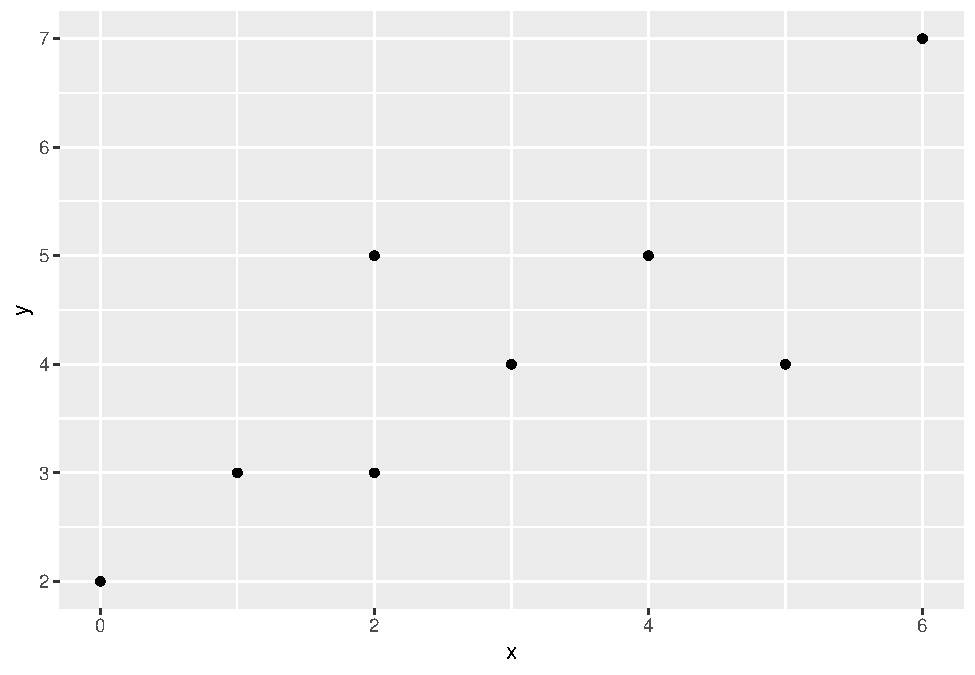
\includegraphics{_main_files/figure-latex/unnamed-chunk-6-1.pdf}

\begin{Shaded}
\begin{Highlighting}[]

\FunctionTok{cov}\NormalTok{(x, y)}
\DocumentationTok{\#\# [1] 2.111111}
\FunctionTok{cor}\NormalTok{(x, y)}
\DocumentationTok{\#\# [1] 0.7680295}
\end{Highlighting}
\end{Shaded}

\hypertarget{ch3}{%
\chapter*{第3章 統計理論の基礎}\label{ch3}}
\addcontentsline{toc}{chapter}{第3章 統計理論の基礎}

第3章では第2章と同じデータを使うため、新たなダウンロードは不要.
なお\href{https://www.yuhikaku.co.jp/books/detail/9784641053854}{出版社サイト}にある第3章のファイルは, 練習問題2-1のデータを用いるところが, 誤って練習問題2-3と同じデータが格納されている.

必要なライブラリを読み込む.

\begin{Shaded}
\begin{Highlighting}[]
\FunctionTok{library}\NormalTok{(tidyverse)}
\end{Highlighting}
\end{Shaded}

\hypertarget{ux7df4ux7fd2ux554fux984c-3-2-ux78baux8a8d}{%
\section*{練習問題 3-2 {[}確認{]}}\label{ux7df4ux7fd2ux554fux984c-3-2-ux78baux8a8d}}
\addcontentsline{toc}{section}{練習問題 3-2 {[}確認{]}}

第2章練習問題2-1で用いたデータを読み込み、両側t検定を実行する.
\(\alpha=0.10\)の場合90\%信頼区間は\([8.354811, 11.645189]\)となり, これは8を含まないことから帰無仮説は棄却できる.
一方で\(\alpha=0.01\)のとき、99\%信頼区間は\([7.277955, 12.722045]\)となり8を含むことから, 帰無仮説は棄却されない.

\begin{Shaded}
\begin{Highlighting}[]
\NormalTok{data32 }\OtherTok{\textless{}{-}} \FunctionTok{read.csv}\NormalTok{(}\StringTok{"data/02\_第2章/02\_practice\_01.csv"}\NormalTok{, }\AttributeTok{header =} \ConstantTok{FALSE}\NormalTok{)}
\NormalTok{x }\OtherTok{\textless{}{-}}\NormalTok{ data32}\SpecialCharTok{$}\NormalTok{V1}

\FunctionTok{t.test}\NormalTok{(x, }\AttributeTok{alternative =} \StringTok{"two.sided"}\NormalTok{, }\AttributeTok{mu =} \DecValTok{8}\NormalTok{, }\AttributeTok{conf.level =} \FloatTok{0.90}\NormalTok{)}
\DocumentationTok{\#\# }
\DocumentationTok{\#\#  One Sample t{-}test}
\DocumentationTok{\#\# }
\DocumentationTok{\#\# data:  x}
\DocumentationTok{\#\# t = 2.102, df = 19, p{-}value = 0.04911}
\DocumentationTok{\#\# alternative hypothesis: true mean is not equal to 8}
\DocumentationTok{\#\# 90 percent confidence interval:}
\DocumentationTok{\#\#   8.354811 11.645189}
\DocumentationTok{\#\# sample estimates:}
\DocumentationTok{\#\# mean of x }
\DocumentationTok{\#\#        10}

\FunctionTok{t.test}\NormalTok{(x, }\AttributeTok{alternative =} \StringTok{"two.sided"}\NormalTok{, }\AttributeTok{mu =} \DecValTok{8}\NormalTok{, }\AttributeTok{conf.level =} \FloatTok{0.99}\NormalTok{)}
\DocumentationTok{\#\# }
\DocumentationTok{\#\#  One Sample t{-}test}
\DocumentationTok{\#\# }
\DocumentationTok{\#\# data:  x}
\DocumentationTok{\#\# t = 2.102, df = 19, p{-}value = 0.04911}
\DocumentationTok{\#\# alternative hypothesis: true mean is not equal to 8}
\DocumentationTok{\#\# 99 percent confidence interval:}
\DocumentationTok{\#\#   7.277955 12.722045}
\DocumentationTok{\#\# sample estimates:}
\DocumentationTok{\#\# mean of x }
\DocumentationTok{\#\#        10}
\end{Highlighting}
\end{Shaded}

\hypertarget{ch4}{%
\chapter*{第4章 線形単回帰モデルの推定と検定}\label{ch4}}
\addcontentsline{toc}{chapter}{第4章 線形単回帰モデルの推定と検定}

先に\href{https://www.yuhikaku.co.jp/books/detail/9784641053854}{出版社サイト}よりデータをダウンロードする.

\begin{Shaded}
\begin{Highlighting}[]
\CommentTok{\# サポートファイルへのリンク}
\NormalTok{curl }\OtherTok{\textless{}{-}} \StringTok{"https://www.yuhikaku.co.jp/static\_files/05385\_support04.zip"}
\CommentTok{\# ダウンロード保存用フォルダが存在しない場合, 作成}
\ControlFlowTok{if}\NormalTok{(}\SpecialCharTok{!}\FunctionTok{dir.exists}\NormalTok{(}\StringTok{"downloads"}\NormalTok{))\{}
    \FunctionTok{dir.create}\NormalTok{(}\StringTok{"downloads"}\NormalTok{)}
\NormalTok{\}}
\NormalTok{cdestfile }\OtherTok{\textless{}{-}} \StringTok{"downloads/support04.zip"}
\FunctionTok{download.file}\NormalTok{(curl, cdestfile)}
\CommentTok{\# データ保存用フォルダが存在しない場合, 作成}
\ControlFlowTok{if}\NormalTok{(}\SpecialCharTok{!}\FunctionTok{dir.exists}\NormalTok{(}\StringTok{"data"}\NormalTok{))\{}
    \FunctionTok{dir.create}\NormalTok{(}\StringTok{"data"}\NormalTok{)}
\NormalTok{\}}
\CommentTok{\# WSL上のRで解凍すると文字化けするので、Linuxのコマンドを外部呼び出し}
\CommentTok{\# Windowsの場合は別途コマンドを用いる.}
\ControlFlowTok{if}\NormalTok{(.Platform}\SpecialCharTok{$}\NormalTok{OS.type }\SpecialCharTok{==} \StringTok{"unix"}\NormalTok{) \{}
    \FunctionTok{system}\NormalTok{(}\FunctionTok{sprintf}\NormalTok{(}\StringTok{\textquotesingle{}unzip {-}n {-}Ocp932 \%s {-}d \%s\textquotesingle{}}\NormalTok{, }\StringTok{"downloads/support04.zip"}\NormalTok{, }\StringTok{"./data"}\NormalTok{))}
\NormalTok{\} }\ControlFlowTok{else}\NormalTok{ \{}
    \FunctionTok{print}\NormalTok{(}\StringTok{"Windowsで解凍するコマンドを別途追加せよ."}\NormalTok{)}
\NormalTok{\}}
\end{Highlighting}
\end{Shaded}

必要なライブラリを読み込む.

\begin{Shaded}
\begin{Highlighting}[]
\FunctionTok{library}\NormalTok{(tidyverse)}
\FunctionTok{library}\NormalTok{(openxlsx)}
\FunctionTok{library}\NormalTok{(estimatr)}
\end{Highlighting}
\end{Shaded}

\hypertarget{ux5b9fux8a3cux4f8b4.1-ux52b4ux50cdux751fux7523ux6027ux3068ux5b9fux8ceaux8cc3ux91d1ux306eux95a2ux4fc2}{%
\section*{実証例4.1 労働生産性と実質賃金の関係}\label{ux5b9fux8a3cux4f8b4.1-ux52b4ux50cdux751fux7523ux6027ux3068ux5b9fux8ceaux8cc3ux91d1ux306eux95a2ux4fc2}}
\addcontentsline{toc}{section}{実証例4.1 労働生産性と実質賃金の関係}

p.128の実証例ブロック内の\(N=22\)は\(N=21\)の誤植と思われる.

\begin{Shaded}
\begin{Highlighting}[]
\NormalTok{ch04\_wage }\OtherTok{\textless{}{-}} \FunctionTok{read.csv}\NormalTok{(}\StringTok{"data/04\_第4章/ch04\_wage.csv"}\NormalTok{)}
\NormalTok{ch04\_wage\_model }\OtherTok{\textless{}{-}} \FunctionTok{lm}\NormalTok{(wage }\SpecialCharTok{\textasciitilde{}}\NormalTok{ productivity, }\AttributeTok{data =}\NormalTok{ ch04\_wage)}
\FunctionTok{summary}\NormalTok{(ch04\_wage\_model)}
\DocumentationTok{\#\# }
\DocumentationTok{\#\# Call:}
\DocumentationTok{\#\# lm(formula = wage \textasciitilde{} productivity, data = ch04\_wage)}
\DocumentationTok{\#\# }
\DocumentationTok{\#\# Residuals:}
\DocumentationTok{\#\#     Min      1Q  Median      3Q     Max }
\DocumentationTok{\#\# {-}47.618 {-}17.612   4.186  21.946  37.052 }
\DocumentationTok{\#\# }
\DocumentationTok{\#\# Coefficients:}
\DocumentationTok{\#\#               Estimate Std. Error t value Pr(\textgreater{}|t|)    }
\DocumentationTok{\#\# (Intercept)  276.12961   87.61057   3.152  0.00525 ** }
\DocumentationTok{\#\# productivity   0.54682    0.02442  22.395 4.04e{-}15 ***}
\DocumentationTok{\#\# {-}{-}{-}}
\DocumentationTok{\#\# Signif. codes:  0 \textquotesingle{}***\textquotesingle{} 0.001 \textquotesingle{}**\textquotesingle{} 0.01 \textquotesingle{}*\textquotesingle{} 0.05 \textquotesingle{}.\textquotesingle{} 0.1 \textquotesingle{} \textquotesingle{} 1}
\DocumentationTok{\#\# }
\DocumentationTok{\#\# Residual standard error: 25.77 on 19 degrees of freedom}
\DocumentationTok{\#\# Multiple R{-}squared:  0.9635, Adjusted R{-}squared:  0.9616 }
\DocumentationTok{\#\# F{-}statistic: 501.5 on 1 and 19 DF,  p{-}value: 4.037e{-}15}
\end{Highlighting}
\end{Shaded}

Rの\texttt{lm()}で計算される標準誤差は不均一分散に対して頑健でない.
本文中にある不均一分散に対して頑健な計算結果を求めるには, \texttt{estimatr::lm\_robust()}を用い, \texttt{se\_type\ =\ "stata"}と指定する.

\begin{Shaded}
\begin{Highlighting}[]
\NormalTok{ch04\_wage\_model\_robust }\OtherTok{\textless{}{-}} \FunctionTok{lm\_robust}\NormalTok{(wage }\SpecialCharTok{\textasciitilde{}}\NormalTok{ productivity, }\AttributeTok{data =}\NormalTok{ ch04\_wage, }\AttributeTok{se\_type =} \StringTok{"stata"}\NormalTok{)}
\FunctionTok{summary}\NormalTok{(ch04\_wage\_model\_robust)}
\DocumentationTok{\#\# }
\DocumentationTok{\#\# Call:}
\DocumentationTok{\#\# lm\_robust(formula = wage \textasciitilde{} productivity, data = ch04\_wage, se\_type = "stata")}
\DocumentationTok{\#\# }
\DocumentationTok{\#\# Standard error type:  HC1 }
\DocumentationTok{\#\# }
\DocumentationTok{\#\# Coefficients:}
\DocumentationTok{\#\#              Estimate Std. Error t value  Pr(\textgreater{}|t|) CI Lower CI Upper DF}
\DocumentationTok{\#\# (Intercept)  276.1296   71.25559   3.875 1.019e{-}03  126.990 425.2693 19}
\DocumentationTok{\#\# productivity   0.5468    0.02046  26.722 1.553e{-}16    0.504   0.5896 19}
\DocumentationTok{\#\# }
\DocumentationTok{\#\# Multiple R{-}squared:  0.9635 ,    Adjusted R{-}squared:  0.9616 }
\DocumentationTok{\#\# F{-}statistic: 714.1 on 1 and 19 DF,  p{-}value: \textless{} 2.2e{-}16}
\end{Highlighting}
\end{Shaded}

\hypertarget{ux56f34-1-ux6642ux9593ux5f53ux305fux308aux5b9fux8ceaux8cc3ux91d1ux3068ux52b4ux50cdux751fux7523ux6027}{%
\section*{図4-1 時間当たり実質賃金と労働生産性}\label{ux56f34-1-ux6642ux9593ux5f53ux305fux308aux5b9fux8ceaux8cc3ux91d1ux3068ux52b4ux50cdux751fux7523ux6027}}
\addcontentsline{toc}{section}{図4-1 時間当たり実質賃金と労働生産性}

回帰曲線は\texttt{geom\_smooth()}で描画できる.

\begin{Shaded}
\begin{Highlighting}[]
\NormalTok{ch04\_wage }\SpecialCharTok{\%\textgreater{}\%}
    \FunctionTok{ggplot}\NormalTok{(}\FunctionTok{aes}\NormalTok{(}\AttributeTok{x =}\NormalTok{ productivity, }\AttributeTok{y =}\NormalTok{ wage)) }\SpecialCharTok{+}
    \FunctionTok{geom\_point}\NormalTok{() }\SpecialCharTok{+}
    \FunctionTok{xlab}\NormalTok{(}\StringTok{"労働生産性 (円)"}\NormalTok{) }\SpecialCharTok{+}
    \FunctionTok{ylab}\NormalTok{(}\StringTok{"実質賃金 (円)"}\NormalTok{) }\SpecialCharTok{+}
    \FunctionTok{geom\_smooth}\NormalTok{(}\AttributeTok{method =} \StringTok{"lm"}\NormalTok{, }\AttributeTok{se =} \ConstantTok{FALSE}\NormalTok{, }\AttributeTok{color =} \StringTok{"black"}\NormalTok{)}
\DocumentationTok{\#\# \textasciigrave{}geom\_smooth()\textasciigrave{} using formula = \textquotesingle{}y \textasciitilde{} x\textquotesingle{}}
\DocumentationTok{\#\# Warning in grid.Call(C\_textBounds, as.graphicsAnnot(x$label), x$x, x$y, :}
\DocumentationTok{\#\# conversion failure on \textquotesingle{}実質賃金 (円)\textquotesingle{} in \textquotesingle{}mbcsToSbcs\textquotesingle{}: dot substituted for \textless{}e5\textgreater{}}
\DocumentationTok{\#\# Warning in grid.Call(C\_textBounds, as.graphicsAnnot(x$label), x$x, x$y, :}
\DocumentationTok{\#\# conversion failure on \textquotesingle{}実質賃金 (円)\textquotesingle{} in \textquotesingle{}mbcsToSbcs\textquotesingle{}: dot substituted for \textless{}ae\textgreater{}}
\DocumentationTok{\#\# Warning in grid.Call(C\_textBounds, as.graphicsAnnot(x$label), x$x, x$y, :}
\DocumentationTok{\#\# conversion failure on \textquotesingle{}実質賃金 (円)\textquotesingle{} in \textquotesingle{}mbcsToSbcs\textquotesingle{}: dot substituted for \textless{}9f\textgreater{}}
\DocumentationTok{\#\# Warning in grid.Call(C\_textBounds, as.graphicsAnnot(x$label), x$x, x$y, :}
\DocumentationTok{\#\# conversion failure on \textquotesingle{}実質賃金 (円)\textquotesingle{} in \textquotesingle{}mbcsToSbcs\textquotesingle{}: dot substituted for \textless{}e8\textgreater{}}
\DocumentationTok{\#\# Warning in grid.Call(C\_textBounds, as.graphicsAnnot(x$label), x$x, x$y, :}
\DocumentationTok{\#\# conversion failure on \textquotesingle{}実質賃金 (円)\textquotesingle{} in \textquotesingle{}mbcsToSbcs\textquotesingle{}: dot substituted for \textless{}b3\textgreater{}}
\DocumentationTok{\#\# Warning in grid.Call(C\_textBounds, as.graphicsAnnot(x$label), x$x, x$y, :}
\DocumentationTok{\#\# conversion failure on \textquotesingle{}実質賃金 (円)\textquotesingle{} in \textquotesingle{}mbcsToSbcs\textquotesingle{}: dot substituted for \textless{}aa\textgreater{}}
\DocumentationTok{\#\# Warning in grid.Call(C\_textBounds, as.graphicsAnnot(x$label), x$x, x$y, :}
\DocumentationTok{\#\# conversion failure on \textquotesingle{}実質賃金 (円)\textquotesingle{} in \textquotesingle{}mbcsToSbcs\textquotesingle{}: dot substituted for \textless{}e8\textgreater{}}
\DocumentationTok{\#\# Warning in grid.Call(C\_textBounds, as.graphicsAnnot(x$label), x$x, x$y, :}
\DocumentationTok{\#\# conversion failure on \textquotesingle{}実質賃金 (円)\textquotesingle{} in \textquotesingle{}mbcsToSbcs\textquotesingle{}: dot substituted for \textless{}b3\textgreater{}}
\DocumentationTok{\#\# Warning in grid.Call(C\_textBounds, as.graphicsAnnot(x$label), x$x, x$y, :}
\DocumentationTok{\#\# conversion failure on \textquotesingle{}実質賃金 (円)\textquotesingle{} in \textquotesingle{}mbcsToSbcs\textquotesingle{}: dot substituted for \textless{}83\textgreater{}}
\DocumentationTok{\#\# Warning in grid.Call(C\_textBounds, as.graphicsAnnot(x$label), x$x, x$y, :}
\DocumentationTok{\#\# conversion failure on \textquotesingle{}実質賃金 (円)\textquotesingle{} in \textquotesingle{}mbcsToSbcs\textquotesingle{}: dot substituted for \textless{}e9\textgreater{}}
\DocumentationTok{\#\# Warning in grid.Call(C\_textBounds, as.graphicsAnnot(x$label), x$x, x$y, :}
\DocumentationTok{\#\# conversion failure on \textquotesingle{}実質賃金 (円)\textquotesingle{} in \textquotesingle{}mbcsToSbcs\textquotesingle{}: dot substituted for \textless{}87\textgreater{}}
\DocumentationTok{\#\# Warning in grid.Call(C\_textBounds, as.graphicsAnnot(x$label), x$x, x$y, :}
\DocumentationTok{\#\# conversion failure on \textquotesingle{}実質賃金 (円)\textquotesingle{} in \textquotesingle{}mbcsToSbcs\textquotesingle{}: dot substituted for \textless{}91\textgreater{}}
\DocumentationTok{\#\# Warning in grid.Call(C\_textBounds, as.graphicsAnnot(x$label), x$x, x$y, :}
\DocumentationTok{\#\# conversion failure on \textquotesingle{}実質賃金 (円)\textquotesingle{} in \textquotesingle{}mbcsToSbcs\textquotesingle{}: dot substituted for \textless{}e5\textgreater{}}
\DocumentationTok{\#\# Warning in grid.Call(C\_textBounds, as.graphicsAnnot(x$label), x$x, x$y, :}
\DocumentationTok{\#\# conversion failure on \textquotesingle{}実質賃金 (円)\textquotesingle{} in \textquotesingle{}mbcsToSbcs\textquotesingle{}: dot substituted for \textless{}86\textgreater{}}

\DocumentationTok{\#\# Warning in grid.Call(C\_textBounds, as.graphicsAnnot(x$label), x$x, x$y, :}
\DocumentationTok{\#\# conversion failure on \textquotesingle{}実質賃金 (円)\textquotesingle{} in \textquotesingle{}mbcsToSbcs\textquotesingle{}: dot substituted for \textless{}86\textgreater{}}
\DocumentationTok{\#\# Warning in grid.Call(C\_textBounds, as.graphicsAnnot(x$label), x$x, x$y, :}
\DocumentationTok{\#\# conversion failure on \textquotesingle{}労働生産性 (円)\textquotesingle{} in \textquotesingle{}mbcsToSbcs\textquotesingle{}: dot substituted for}
\DocumentationTok{\#\# \textless{}e5\textgreater{}}
\DocumentationTok{\#\# Warning in grid.Call(C\_textBounds, as.graphicsAnnot(x$label), x$x, x$y, :}
\DocumentationTok{\#\# conversion failure on \textquotesingle{}労働生産性 (円)\textquotesingle{} in \textquotesingle{}mbcsToSbcs\textquotesingle{}: dot substituted for}
\DocumentationTok{\#\# \textless{}8a\textgreater{}}
\DocumentationTok{\#\# Warning in grid.Call(C\_textBounds, as.graphicsAnnot(x$label), x$x, x$y, :}
\DocumentationTok{\#\# conversion failure on \textquotesingle{}労働生産性 (円)\textquotesingle{} in \textquotesingle{}mbcsToSbcs\textquotesingle{}: dot substituted for}
\DocumentationTok{\#\# \textless{}b4\textgreater{}}
\DocumentationTok{\#\# Warning in grid.Call(C\_textBounds, as.graphicsAnnot(x$label), x$x, x$y, :}
\DocumentationTok{\#\# conversion failure on \textquotesingle{}労働生産性 (円)\textquotesingle{} in \textquotesingle{}mbcsToSbcs\textquotesingle{}: dot substituted for}
\DocumentationTok{\#\# \textless{}e5\textgreater{}}
\DocumentationTok{\#\# Warning in grid.Call(C\_textBounds, as.graphicsAnnot(x$label), x$x, x$y, :}
\DocumentationTok{\#\# conversion failure on \textquotesingle{}労働生産性 (円)\textquotesingle{} in \textquotesingle{}mbcsToSbcs\textquotesingle{}: dot substituted for}
\DocumentationTok{\#\# \textless{}83\textgreater{}}
\DocumentationTok{\#\# Warning in grid.Call(C\_textBounds, as.graphicsAnnot(x$label), x$x, x$y, :}
\DocumentationTok{\#\# conversion failure on \textquotesingle{}労働生産性 (円)\textquotesingle{} in \textquotesingle{}mbcsToSbcs\textquotesingle{}: dot substituted for}
\DocumentationTok{\#\# \textless{}8d\textgreater{}}
\DocumentationTok{\#\# Warning in grid.Call(C\_textBounds, as.graphicsAnnot(x$label), x$x, x$y, :}
\DocumentationTok{\#\# conversion failure on \textquotesingle{}労働生産性 (円)\textquotesingle{} in \textquotesingle{}mbcsToSbcs\textquotesingle{}: dot substituted for}
\DocumentationTok{\#\# \textless{}e7\textgreater{}}
\DocumentationTok{\#\# Warning in grid.Call(C\_textBounds, as.graphicsAnnot(x$label), x$x, x$y, :}
\DocumentationTok{\#\# conversion failure on \textquotesingle{}労働生産性 (円)\textquotesingle{} in \textquotesingle{}mbcsToSbcs\textquotesingle{}: dot substituted for}
\DocumentationTok{\#\# \textless{}94\textgreater{}}
\DocumentationTok{\#\# Warning in grid.Call(C\_textBounds, as.graphicsAnnot(x$label), x$x, x$y, :}
\DocumentationTok{\#\# conversion failure on \textquotesingle{}労働生産性 (円)\textquotesingle{} in \textquotesingle{}mbcsToSbcs\textquotesingle{}: dot substituted for}
\DocumentationTok{\#\# \textless{}9f\textgreater{}}
\DocumentationTok{\#\# Warning in grid.Call(C\_textBounds, as.graphicsAnnot(x$label), x$x, x$y, :}
\DocumentationTok{\#\# conversion failure on \textquotesingle{}労働生産性 (円)\textquotesingle{} in \textquotesingle{}mbcsToSbcs\textquotesingle{}: dot substituted for}
\DocumentationTok{\#\# \textless{}e7\textgreater{}}
\DocumentationTok{\#\# Warning in grid.Call(C\_textBounds, as.graphicsAnnot(x$label), x$x, x$y, :}
\DocumentationTok{\#\# conversion failure on \textquotesingle{}労働生産性 (円)\textquotesingle{} in \textquotesingle{}mbcsToSbcs\textquotesingle{}: dot substituted for}
\DocumentationTok{\#\# \textless{}94\textgreater{}}
\DocumentationTok{\#\# Warning in grid.Call(C\_textBounds, as.graphicsAnnot(x$label), x$x, x$y, :}
\DocumentationTok{\#\# conversion failure on \textquotesingle{}労働生産性 (円)\textquotesingle{} in \textquotesingle{}mbcsToSbcs\textquotesingle{}: dot substituted for}
\DocumentationTok{\#\# \textless{}a3\textgreater{}}
\DocumentationTok{\#\# Warning in grid.Call(C\_textBounds, as.graphicsAnnot(x$label), x$x, x$y, :}
\DocumentationTok{\#\# conversion failure on \textquotesingle{}労働生産性 (円)\textquotesingle{} in \textquotesingle{}mbcsToSbcs\textquotesingle{}: dot substituted for}
\DocumentationTok{\#\# \textless{}e6\textgreater{}}
\DocumentationTok{\#\# Warning in grid.Call(C\_textBounds, as.graphicsAnnot(x$label), x$x, x$y, :}
\DocumentationTok{\#\# conversion failure on \textquotesingle{}労働生産性 (円)\textquotesingle{} in \textquotesingle{}mbcsToSbcs\textquotesingle{}: dot substituted for}
\DocumentationTok{\#\# \textless{}80\textgreater{}}
\DocumentationTok{\#\# Warning in grid.Call(C\_textBounds, as.graphicsAnnot(x$label), x$x, x$y, :}
\DocumentationTok{\#\# conversion failure on \textquotesingle{}労働生産性 (円)\textquotesingle{} in \textquotesingle{}mbcsToSbcs\textquotesingle{}: dot substituted for}
\DocumentationTok{\#\# \textless{}a7\textgreater{}}
\DocumentationTok{\#\# Warning in grid.Call(C\_textBounds, as.graphicsAnnot(x$label), x$x, x$y, :}
\DocumentationTok{\#\# conversion failure on \textquotesingle{}労働生産性 (円)\textquotesingle{} in \textquotesingle{}mbcsToSbcs\textquotesingle{}: dot substituted for}
\DocumentationTok{\#\# \textless{}e5\textgreater{}}
\DocumentationTok{\#\# Warning in grid.Call(C\_textBounds, as.graphicsAnnot(x$label), x$x, x$y, :}
\DocumentationTok{\#\# conversion failure on \textquotesingle{}労働生産性 (円)\textquotesingle{} in \textquotesingle{}mbcsToSbcs\textquotesingle{}: dot substituted for}
\DocumentationTok{\#\# \textless{}86\textgreater{}}

\DocumentationTok{\#\# Warning in grid.Call(C\_textBounds, as.graphicsAnnot(x$label), x$x, x$y, :}
\DocumentationTok{\#\# conversion failure on \textquotesingle{}労働生産性 (円)\textquotesingle{} in \textquotesingle{}mbcsToSbcs\textquotesingle{}: dot substituted for}
\DocumentationTok{\#\# \textless{}86\textgreater{}}
\DocumentationTok{\#\# Warning in grid.Call.graphics(C\_text, as.graphicsAnnot(x$label), x$x, x$y, :}
\DocumentationTok{\#\# conversion failure on \textquotesingle{}労働生産性 (円)\textquotesingle{} in \textquotesingle{}mbcsToSbcs\textquotesingle{}: dot substituted for}
\DocumentationTok{\#\# \textless{}e5\textgreater{}}
\DocumentationTok{\#\# Warning in grid.Call.graphics(C\_text, as.graphicsAnnot(x$label), x$x, x$y, :}
\DocumentationTok{\#\# conversion failure on \textquotesingle{}労働生産性 (円)\textquotesingle{} in \textquotesingle{}mbcsToSbcs\textquotesingle{}: dot substituted for}
\DocumentationTok{\#\# \textless{}8a\textgreater{}}
\DocumentationTok{\#\# Warning in grid.Call.graphics(C\_text, as.graphicsAnnot(x$label), x$x, x$y, :}
\DocumentationTok{\#\# conversion failure on \textquotesingle{}労働生産性 (円)\textquotesingle{} in \textquotesingle{}mbcsToSbcs\textquotesingle{}: dot substituted for}
\DocumentationTok{\#\# \textless{}b4\textgreater{}}
\DocumentationTok{\#\# Warning in grid.Call.graphics(C\_text, as.graphicsAnnot(x$label), x$x, x$y, :}
\DocumentationTok{\#\# conversion failure on \textquotesingle{}労働生産性 (円)\textquotesingle{} in \textquotesingle{}mbcsToSbcs\textquotesingle{}: dot substituted for}
\DocumentationTok{\#\# \textless{}e5\textgreater{}}
\DocumentationTok{\#\# Warning in grid.Call.graphics(C\_text, as.graphicsAnnot(x$label), x$x, x$y, :}
\DocumentationTok{\#\# conversion failure on \textquotesingle{}労働生産性 (円)\textquotesingle{} in \textquotesingle{}mbcsToSbcs\textquotesingle{}: dot substituted for}
\DocumentationTok{\#\# \textless{}83\textgreater{}}
\DocumentationTok{\#\# Warning in grid.Call.graphics(C\_text, as.graphicsAnnot(x$label), x$x, x$y, :}
\DocumentationTok{\#\# conversion failure on \textquotesingle{}労働生産性 (円)\textquotesingle{} in \textquotesingle{}mbcsToSbcs\textquotesingle{}: dot substituted for}
\DocumentationTok{\#\# \textless{}8d\textgreater{}}
\DocumentationTok{\#\# Warning in grid.Call.graphics(C\_text, as.graphicsAnnot(x$label), x$x, x$y, :}
\DocumentationTok{\#\# conversion failure on \textquotesingle{}労働生産性 (円)\textquotesingle{} in \textquotesingle{}mbcsToSbcs\textquotesingle{}: dot substituted for}
\DocumentationTok{\#\# \textless{}e7\textgreater{}}
\DocumentationTok{\#\# Warning in grid.Call.graphics(C\_text, as.graphicsAnnot(x$label), x$x, x$y, :}
\DocumentationTok{\#\# conversion failure on \textquotesingle{}労働生産性 (円)\textquotesingle{} in \textquotesingle{}mbcsToSbcs\textquotesingle{}: dot substituted for}
\DocumentationTok{\#\# \textless{}94\textgreater{}}
\DocumentationTok{\#\# Warning in grid.Call.graphics(C\_text, as.graphicsAnnot(x$label), x$x, x$y, :}
\DocumentationTok{\#\# conversion failure on \textquotesingle{}労働生産性 (円)\textquotesingle{} in \textquotesingle{}mbcsToSbcs\textquotesingle{}: dot substituted for}
\DocumentationTok{\#\# \textless{}9f\textgreater{}}
\DocumentationTok{\#\# Warning in grid.Call.graphics(C\_text, as.graphicsAnnot(x$label), x$x, x$y, :}
\DocumentationTok{\#\# conversion failure on \textquotesingle{}労働生産性 (円)\textquotesingle{} in \textquotesingle{}mbcsToSbcs\textquotesingle{}: dot substituted for}
\DocumentationTok{\#\# \textless{}e7\textgreater{}}
\DocumentationTok{\#\# Warning in grid.Call.graphics(C\_text, as.graphicsAnnot(x$label), x$x, x$y, :}
\DocumentationTok{\#\# conversion failure on \textquotesingle{}労働生産性 (円)\textquotesingle{} in \textquotesingle{}mbcsToSbcs\textquotesingle{}: dot substituted for}
\DocumentationTok{\#\# \textless{}94\textgreater{}}
\DocumentationTok{\#\# Warning in grid.Call.graphics(C\_text, as.graphicsAnnot(x$label), x$x, x$y, :}
\DocumentationTok{\#\# conversion failure on \textquotesingle{}労働生産性 (円)\textquotesingle{} in \textquotesingle{}mbcsToSbcs\textquotesingle{}: dot substituted for}
\DocumentationTok{\#\# \textless{}a3\textgreater{}}
\DocumentationTok{\#\# Warning in grid.Call.graphics(C\_text, as.graphicsAnnot(x$label), x$x, x$y, :}
\DocumentationTok{\#\# conversion failure on \textquotesingle{}労働生産性 (円)\textquotesingle{} in \textquotesingle{}mbcsToSbcs\textquotesingle{}: dot substituted for}
\DocumentationTok{\#\# \textless{}e6\textgreater{}}
\DocumentationTok{\#\# Warning in grid.Call.graphics(C\_text, as.graphicsAnnot(x$label), x$x, x$y, :}
\DocumentationTok{\#\# conversion failure on \textquotesingle{}労働生産性 (円)\textquotesingle{} in \textquotesingle{}mbcsToSbcs\textquotesingle{}: dot substituted for}
\DocumentationTok{\#\# \textless{}80\textgreater{}}
\DocumentationTok{\#\# Warning in grid.Call.graphics(C\_text, as.graphicsAnnot(x$label), x$x, x$y, :}
\DocumentationTok{\#\# conversion failure on \textquotesingle{}労働生産性 (円)\textquotesingle{} in \textquotesingle{}mbcsToSbcs\textquotesingle{}: dot substituted for}
\DocumentationTok{\#\# \textless{}a7\textgreater{}}
\DocumentationTok{\#\# Warning in grid.Call.graphics(C\_text, as.graphicsAnnot(x$label), x$x, x$y, :}
\DocumentationTok{\#\# conversion failure on \textquotesingle{}労働生産性 (円)\textquotesingle{} in \textquotesingle{}mbcsToSbcs\textquotesingle{}: dot substituted for}
\DocumentationTok{\#\# \textless{}e5\textgreater{}}
\DocumentationTok{\#\# Warning in grid.Call.graphics(C\_text, as.graphicsAnnot(x$label), x$x, x$y, :}
\DocumentationTok{\#\# conversion failure on \textquotesingle{}労働生産性 (円)\textquotesingle{} in \textquotesingle{}mbcsToSbcs\textquotesingle{}: dot substituted for}
\DocumentationTok{\#\# \textless{}86\textgreater{}}

\DocumentationTok{\#\# Warning in grid.Call.graphics(C\_text, as.graphicsAnnot(x$label), x$x, x$y, :}
\DocumentationTok{\#\# conversion failure on \textquotesingle{}労働生産性 (円)\textquotesingle{} in \textquotesingle{}mbcsToSbcs\textquotesingle{}: dot substituted for}
\DocumentationTok{\#\# \textless{}86\textgreater{}}
\DocumentationTok{\#\# Warning in grid.Call.graphics(C\_text, as.graphicsAnnot(x$label), x$x, x$y, :}
\DocumentationTok{\#\# conversion failure on \textquotesingle{}実質賃金 (円)\textquotesingle{} in \textquotesingle{}mbcsToSbcs\textquotesingle{}: dot substituted for \textless{}e5\textgreater{}}
\DocumentationTok{\#\# Warning in grid.Call.graphics(C\_text, as.graphicsAnnot(x$label), x$x, x$y, :}
\DocumentationTok{\#\# conversion failure on \textquotesingle{}実質賃金 (円)\textquotesingle{} in \textquotesingle{}mbcsToSbcs\textquotesingle{}: dot substituted for \textless{}ae\textgreater{}}
\DocumentationTok{\#\# Warning in grid.Call.graphics(C\_text, as.graphicsAnnot(x$label), x$x, x$y, :}
\DocumentationTok{\#\# conversion failure on \textquotesingle{}実質賃金 (円)\textquotesingle{} in \textquotesingle{}mbcsToSbcs\textquotesingle{}: dot substituted for \textless{}9f\textgreater{}}
\DocumentationTok{\#\# Warning in grid.Call.graphics(C\_text, as.graphicsAnnot(x$label), x$x, x$y, :}
\DocumentationTok{\#\# conversion failure on \textquotesingle{}実質賃金 (円)\textquotesingle{} in \textquotesingle{}mbcsToSbcs\textquotesingle{}: dot substituted for \textless{}e8\textgreater{}}
\DocumentationTok{\#\# Warning in grid.Call.graphics(C\_text, as.graphicsAnnot(x$label), x$x, x$y, :}
\DocumentationTok{\#\# conversion failure on \textquotesingle{}実質賃金 (円)\textquotesingle{} in \textquotesingle{}mbcsToSbcs\textquotesingle{}: dot substituted for \textless{}b3\textgreater{}}
\DocumentationTok{\#\# Warning in grid.Call.graphics(C\_text, as.graphicsAnnot(x$label), x$x, x$y, :}
\DocumentationTok{\#\# conversion failure on \textquotesingle{}実質賃金 (円)\textquotesingle{} in \textquotesingle{}mbcsToSbcs\textquotesingle{}: dot substituted for \textless{}aa\textgreater{}}
\DocumentationTok{\#\# Warning in grid.Call.graphics(C\_text, as.graphicsAnnot(x$label), x$x, x$y, :}
\DocumentationTok{\#\# conversion failure on \textquotesingle{}実質賃金 (円)\textquotesingle{} in \textquotesingle{}mbcsToSbcs\textquotesingle{}: dot substituted for \textless{}e8\textgreater{}}
\DocumentationTok{\#\# Warning in grid.Call.graphics(C\_text, as.graphicsAnnot(x$label), x$x, x$y, :}
\DocumentationTok{\#\# conversion failure on \textquotesingle{}実質賃金 (円)\textquotesingle{} in \textquotesingle{}mbcsToSbcs\textquotesingle{}: dot substituted for \textless{}b3\textgreater{}}
\DocumentationTok{\#\# Warning in grid.Call.graphics(C\_text, as.graphicsAnnot(x$label), x$x, x$y, :}
\DocumentationTok{\#\# conversion failure on \textquotesingle{}実質賃金 (円)\textquotesingle{} in \textquotesingle{}mbcsToSbcs\textquotesingle{}: dot substituted for \textless{}83\textgreater{}}
\DocumentationTok{\#\# Warning in grid.Call.graphics(C\_text, as.graphicsAnnot(x$label), x$x, x$y, :}
\DocumentationTok{\#\# conversion failure on \textquotesingle{}実質賃金 (円)\textquotesingle{} in \textquotesingle{}mbcsToSbcs\textquotesingle{}: dot substituted for \textless{}e9\textgreater{}}
\DocumentationTok{\#\# Warning in grid.Call.graphics(C\_text, as.graphicsAnnot(x$label), x$x, x$y, :}
\DocumentationTok{\#\# conversion failure on \textquotesingle{}実質賃金 (円)\textquotesingle{} in \textquotesingle{}mbcsToSbcs\textquotesingle{}: dot substituted for \textless{}87\textgreater{}}
\DocumentationTok{\#\# Warning in grid.Call.graphics(C\_text, as.graphicsAnnot(x$label), x$x, x$y, :}
\DocumentationTok{\#\# conversion failure on \textquotesingle{}実質賃金 (円)\textquotesingle{} in \textquotesingle{}mbcsToSbcs\textquotesingle{}: dot substituted for \textless{}91\textgreater{}}
\DocumentationTok{\#\# Warning in grid.Call.graphics(C\_text, as.graphicsAnnot(x$label), x$x, x$y, :}
\DocumentationTok{\#\# conversion failure on \textquotesingle{}実質賃金 (円)\textquotesingle{} in \textquotesingle{}mbcsToSbcs\textquotesingle{}: dot substituted for \textless{}e5\textgreater{}}
\DocumentationTok{\#\# Warning in grid.Call.graphics(C\_text, as.graphicsAnnot(x$label), x$x, x$y, :}
\DocumentationTok{\#\# conversion failure on \textquotesingle{}実質賃金 (円)\textquotesingle{} in \textquotesingle{}mbcsToSbcs\textquotesingle{}: dot substituted for \textless{}86\textgreater{}}

\DocumentationTok{\#\# Warning in grid.Call.graphics(C\_text, as.graphicsAnnot(x$label), x$x, x$y, :}
\DocumentationTok{\#\# conversion failure on \textquotesingle{}実質賃金 (円)\textquotesingle{} in \textquotesingle{}mbcsToSbcs\textquotesingle{}: dot substituted for \textless{}86\textgreater{}}
\end{Highlighting}
\end{Shaded}

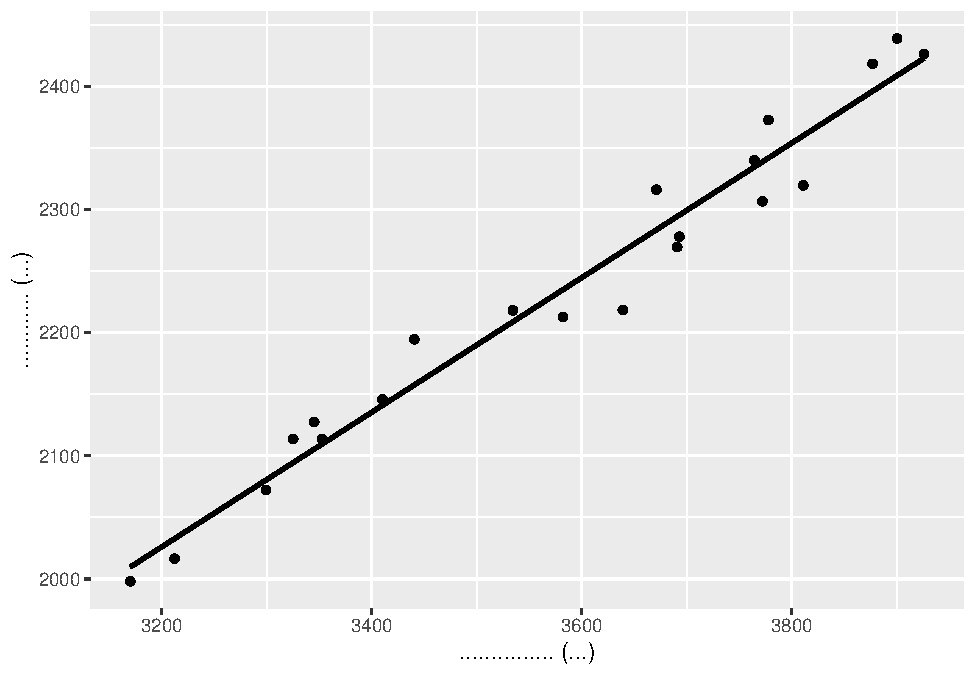
\includegraphics{_main_files/figure-latex/unnamed-chunk-13-1.pdf}

\hypertarget{ux7df4ux7fd2ux554fux984c-4-2-ux5b9fux8a3c}{%
\section*{練習問題 4-2 {[}実証{]}}\label{ux7df4ux7fd2ux554fux984c-4-2-ux5b9fux8a3c}}
\addcontentsline{toc}{section}{練習問題 4-2 {[}実証{]}}

\begin{enumerate}
\def\labelenumi{(\arabic{enumi})}
\tightlist
\item
  データを読み込み, 回帰分析を実行する.
  Excelファイルの読み込みには\texttt{openxlsx::read.xlsx()}を用いる.
  列名が日本語だと扱いづらいため, これを変更しておく.
  \(gdp2013\_ln = \beta_0 + \beta_1 pop2013\_ln\)というモデルを立てると, \(\hat{\beta_0} = 7.623, \hat{\beta_1} = 1.075\)と求められる.
\end{enumerate}

\begin{Shaded}
\begin{Highlighting}[]
\NormalTok{data42 }\OtherTok{\textless{}{-}} \FunctionTok{read.xlsx}\NormalTok{(}\StringTok{"data/04\_第4章/data for chap 4 exercise 2.xlsx"}\NormalTok{)}
\FunctionTok{colnames}\NormalTok{(data42) }\OtherTok{\textless{}{-}} \FunctionTok{c}\NormalTok{(}\StringTok{"pref"}\NormalTok{, }\StringTok{"pop2013"}\NormalTok{, }\StringTok{"gdp2013"}\NormalTok{, }\StringTok{"pop2013\_ln"}\NormalTok{, }\StringTok{"gdp2013\_ln"}\NormalTok{)}

\NormalTok{model42 }\OtherTok{\textless{}{-}} \FunctionTok{lm}\NormalTok{(gdp2013\_ln }\SpecialCharTok{\textasciitilde{}}\NormalTok{ pop2013\_ln, }\AttributeTok{data =}\NormalTok{ data42)}
\NormalTok{model42}
\DocumentationTok{\#\# }
\DocumentationTok{\#\# Call:}
\DocumentationTok{\#\# lm(formula = gdp2013\_ln \textasciitilde{} pop2013\_ln, data = data42)}
\DocumentationTok{\#\# }
\DocumentationTok{\#\# Coefficients:}
\DocumentationTok{\#\# (Intercept)   pop2013\_ln  }
\DocumentationTok{\#\#       7.623        1.075}
\end{Highlighting}
\end{Shaded}

\begin{enumerate}
\def\labelenumi{(\arabic{enumi})}
\setcounter{enumi}{1}
\tightlist
\item
  帰無仮説\(H_0\): \(\beta_1 = 1\)に関して, 統計量\(t = \frac{\hat{\beta_1} - \beta_1}{\text{SE}(\hat{\beta_1})} = 2.62773\)が求められる.
  これは自由度\(n-2 = 45\)で, 有意水準5\%のt検定の棄却域\((\infty, -2.014103]\), \([2.014103, \infty)\)に入っていることから帰無仮説は棄却される.
\end{enumerate}

\begin{Shaded}
\begin{Highlighting}[]
\NormalTok{beta1 }\OtherTok{\textless{}{-}}\NormalTok{ model42}\SpecialCharTok{$}\NormalTok{coefficients[}\DecValTok{2}\NormalTok{]}
\NormalTok{sebeta1 }\OtherTok{\textless{}{-}} \FunctionTok{summary}\NormalTok{(model42)}\SpecialCharTok{$}\NormalTok{coefficients[}\DecValTok{2}\NormalTok{, }\DecValTok{2}\NormalTok{]}
\NormalTok{n }\OtherTok{\textless{}{-}} \FunctionTok{dim}\NormalTok{(data42)[}\DecValTok{1}\NormalTok{]}

\NormalTok{t }\OtherTok{\textless{}{-}}\NormalTok{ (beta1 }\SpecialCharTok{{-}} \DecValTok{1}\NormalTok{)}\SpecialCharTok{/}\NormalTok{sebeta1}
\NormalTok{t}
\DocumentationTok{\#\# pop2013\_ln }
\DocumentationTok{\#\#    2.62773}
\FunctionTok{qt}\NormalTok{(}\FloatTok{0.975}\NormalTok{, n}\DecValTok{{-}2}\NormalTok{) }\CommentTok{\# 2.014103}
\DocumentationTok{\#\# [1] 2.014103}
\end{Highlighting}
\end{Shaded}

\begin{enumerate}
\def\labelenumi{(\arabic{enumi})}
\setcounter{enumi}{2}
\tightlist
\item
  \texttt{confint()}関数を用いると直接求められる.
\end{enumerate}

\begin{Shaded}
\begin{Highlighting}[]
\FunctionTok{confint}\NormalTok{(model42, }\StringTok{\textquotesingle{}(Intercept)\textquotesingle{}}\NormalTok{, }\AttributeTok{level=}\FloatTok{0.90}\NormalTok{)}
\DocumentationTok{\#\#                  5 \%     95 \%}
\DocumentationTok{\#\# (Intercept) 7.257252 7.988132}
\end{Highlighting}
\end{Shaded}

\begin{enumerate}
\def\labelenumi{(\arabic{enumi})}
\setcounter{enumi}{3}
\item
  人口が1\%変化すると, GDPは\(\beta_1 = 1.075\)\%変化する.
\item
  \(\text{Var}(u) = \frac{\sum_{i=1}^n \hat{u}_i^2}{n-2} = 0.02245859\)と求められる.
  ln(人口)の分散は\texttt{var()}関数を用いると, 0.5964525と求められる.
\end{enumerate}

\begin{Shaded}
\begin{Highlighting}[]
\FunctionTok{sum}\NormalTok{(model42}\SpecialCharTok{$}\NormalTok{residuals}\SpecialCharTok{\^{}}\DecValTok{2}\NormalTok{)}\SpecialCharTok{/}\NormalTok{(n}\DecValTok{{-}2}\NormalTok{)}
\DocumentationTok{\#\# [1] 0.02245859}

\NormalTok{var\_pop2013\_ln }\OtherTok{\textless{}{-}} \FunctionTok{var}\NormalTok{(data42}\SpecialCharTok{$}\NormalTok{pop2013\_ln)}
\NormalTok{var\_pop2013\_ln}
\DocumentationTok{\#\# [1] 0.5964525}
\end{Highlighting}
\end{Shaded}

\hypertarget{ux7df4ux7fd2ux554fux984c-4-10-ux5b9fux8a3c}{%
\section*{練習問題 4-10 {[}実証{]}}\label{ux7df4ux7fd2ux554fux984c-4-10-ux5b9fux8a3c}}
\addcontentsline{toc}{section}{練習問題 4-10 {[}実証{]}}

\begin{enumerate}
\def\labelenumi{(\arabic{enumi})}
\tightlist
\item
  データを読み込み, 回帰分析を実行することで\(\beta_1\)を一致推定できるか調べる.
  実際に計算すると, Cov\((u_i, X_i) = 0\)が成り立っていることが確認できる.
\end{enumerate}

\begin{Shaded}
\begin{Highlighting}[]
\NormalTok{data410 }\OtherTok{\textless{}{-}} \FunctionTok{read.xlsx}\NormalTok{(}\StringTok{"data/04\_第4章/data for chap 4 exercise 10.xlsx"}\NormalTok{) }\SpecialCharTok{\%\textgreater{}\%} \FunctionTok{data.frame}\NormalTok{()}
\NormalTok{model410 }\OtherTok{\textless{}{-}} \FunctionTok{lm}\NormalTok{(Y }\SpecialCharTok{\textasciitilde{}}\NormalTok{ X, }\AttributeTok{data =}\NormalTok{ data410)}
\FunctionTok{cov}\NormalTok{(model410}\SpecialCharTok{$}\NormalTok{residuals, data410}\SpecialCharTok{$}\NormalTok{X)}
\DocumentationTok{\#\# [1] 4.392411e{-}18}
\end{Highlighting}
\end{Shaded}

\begin{enumerate}
\def\labelenumi{(\arabic{enumi})}
\setcounter{enumi}{1}
\tightlist
\item
  E\((u_i^2|X_i) = 0.690318 \neq 0\).
  散布図を描くと, \(\hat{Y}_i\)が大きくなるに従って残差の分散が大きくなっていることが確認できる.
\end{enumerate}

\begin{Shaded}
\begin{Highlighting}[]
\FunctionTok{mean}\NormalTok{(model410}\SpecialCharTok{$}\NormalTok{residuals}\SpecialCharTok{\^{}}\DecValTok{2}\NormalTok{)}
\DocumentationTok{\#\# [1] 0.690318}

\NormalTok{model410 }\SpecialCharTok{\%\textgreater{}\%}
    \FunctionTok{ggplot}\NormalTok{(}\FunctionTok{aes}\NormalTok{(}\AttributeTok{x =}\NormalTok{ .fitted, }\AttributeTok{y =}\NormalTok{ .resid)) }\SpecialCharTok{+}
    \FunctionTok{geom\_point}\NormalTok{() }\SpecialCharTok{+}
    \FunctionTok{geom\_hline}\NormalTok{(}\AttributeTok{yintercept =} \DecValTok{0}\NormalTok{)}
\end{Highlighting}
\end{Shaded}

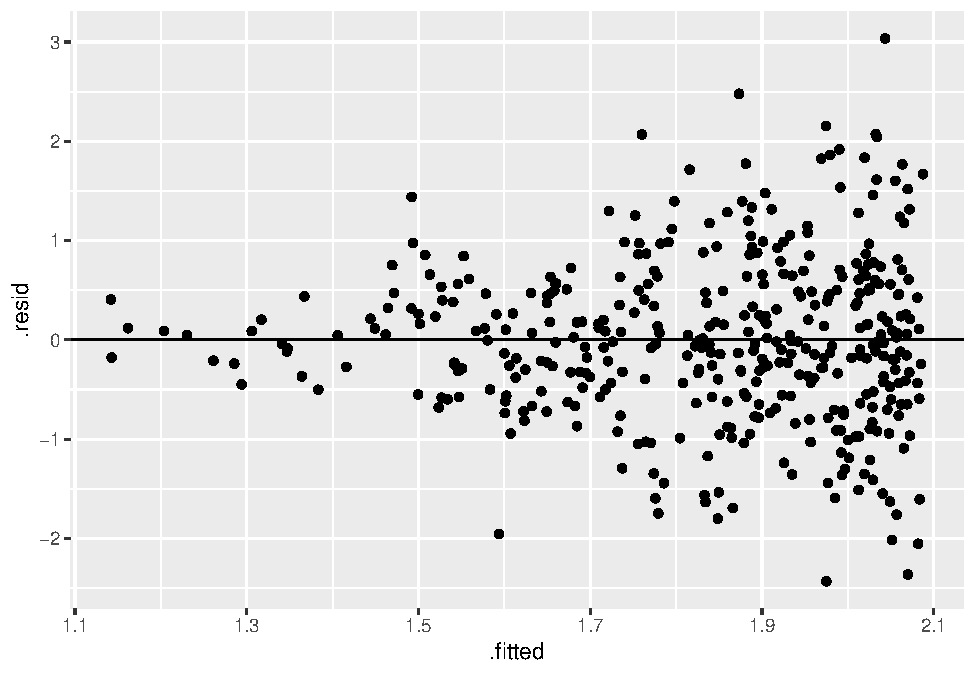
\includegraphics{_main_files/figure-latex/unnamed-chunk-19-1.pdf}

\begin{enumerate}
\def\labelenumi{(\arabic{enumi})}
\setcounter{enumi}{2}
\tightlist
\item
  不均一分散に頑健な標準誤差は\texttt{estimatr::lm\_robust()}を用いて求める.
\end{enumerate}

\begin{Shaded}
\begin{Highlighting}[]
\NormalTok{model410\_robust }\OtherTok{\textless{}{-}} \FunctionTok{lm\_robust}\NormalTok{(Y }\SpecialCharTok{\textasciitilde{}}\NormalTok{ X, }\AttributeTok{data =}\NormalTok{ data410)}
\FunctionTok{summary}\NormalTok{(model410\_robust)}
\DocumentationTok{\#\# }
\DocumentationTok{\#\# Call:}
\DocumentationTok{\#\# lm\_robust(formula = Y \textasciitilde{} X, data = data410)}
\DocumentationTok{\#\# }
\DocumentationTok{\#\# Standard error type:  HC2 }
\DocumentationTok{\#\# }
\DocumentationTok{\#\# Coefficients:}
\DocumentationTok{\#\#             Estimate Std. Error t value  Pr(\textgreater{}|t|) CI Lower CI Upper  DF}
\DocumentationTok{\#\# (Intercept)   0.8103     0.1583   5.119 4.803e{-}07   0.4991    1.122 398}
\DocumentationTok{\#\# X             1.2773     0.2158   5.918 7.035e{-}09   0.8530    1.702 398}
\DocumentationTok{\#\# }
\DocumentationTok{\#\# Multiple R{-}squared:  0.05683 ,   Adjusted R{-}squared:  0.05446 }
\DocumentationTok{\#\# F{-}statistic: 35.02 on 1 and 398 DF,  p{-}value: 7.035e{-}09}
\end{Highlighting}
\end{Shaded}

\texttt{summary()}によると, \(\beta_1\)の95\%信頼区間に0.8は入っていないため, 帰無仮説は棄却されない.

\begin{enumerate}
\def\labelenumi{(\arabic{enumi})}
\setcounter{enumi}{3}
\tightlist
\item
  不均一分散に頑健な標準誤差は\texttt{estimatr::lm\_robust()}を用いて求める.
\end{enumerate}

\begin{Shaded}
\begin{Highlighting}[]
\FunctionTok{confint}\NormalTok{(model410)}
\DocumentationTok{\#\#                 2.5 \%   97.5 \%}
\DocumentationTok{\#\# (Intercept) 0.3912772 1.229412}
\DocumentationTok{\#\# X           0.7645056 1.790022}
\end{Highlighting}
\end{Shaded}

\texttt{summary()}によると, \(\beta_1\)の95\%信頼区間に0.8は入っており, 帰無仮説は棄却される.

\begin{enumerate}
\def\labelenumi{(\arabic{enumi})}
\setcounter{enumi}{4}
\tightlist
\item
  分散が均一でないデータに均一分散を仮定した標準誤差を用いると, 上のように異なる結果が導かれることがある.
\end{enumerate}

\hypertarget{ch5}{%
\chapter*{第5章 重回帰モデルの推定と検定}\label{ch5}}
\addcontentsline{toc}{chapter}{第5章 重回帰モデルの推定と検定}

先に\href{https://www.yuhikaku.co.jp/books/detail/9784641053854}{出版社サイト}よりデータをダウンロードする.

\begin{Shaded}
\begin{Highlighting}[]
\CommentTok{\# サポートファイルへのリンク}
\NormalTok{curl }\OtherTok{\textless{}{-}} \StringTok{"https://www.yuhikaku.co.jp/static\_files/05385\_support05.zip"}
\CommentTok{\# ダウンロード保存用フォルダが存在しない場合, 作成}
\ControlFlowTok{if}\NormalTok{(}\SpecialCharTok{!}\FunctionTok{dir.exists}\NormalTok{(}\StringTok{"downloads"}\NormalTok{))\{}
    \FunctionTok{dir.create}\NormalTok{(}\StringTok{"downloads"}\NormalTok{)}
\NormalTok{\}}
\NormalTok{cdestfile }\OtherTok{\textless{}{-}} \StringTok{"downloads/support05.zip"}
\FunctionTok{download.file}\NormalTok{(curl, cdestfile)}
\CommentTok{\# データ保存用フォルダが存在しない場合, 作成}
\ControlFlowTok{if}\NormalTok{(}\SpecialCharTok{!}\FunctionTok{dir.exists}\NormalTok{(}\StringTok{"data"}\NormalTok{))\{}
    \FunctionTok{dir.create}\NormalTok{(}\StringTok{"data"}\NormalTok{)}
\NormalTok{\}}
\CommentTok{\# WSL上のRで解凍すると文字化けするので、Linuxのコマンドを外部呼び出し}
\CommentTok{\# Windowsの場合は別途コマンドを用いる.}
\ControlFlowTok{if}\NormalTok{(.Platform}\SpecialCharTok{$}\NormalTok{OS.type }\SpecialCharTok{==} \StringTok{"unix"}\NormalTok{) \{}
    \FunctionTok{system}\NormalTok{(}\FunctionTok{sprintf}\NormalTok{(}\StringTok{\textquotesingle{}unzip {-}n {-}Ocp932 \%s {-}d \%s\textquotesingle{}}\NormalTok{, }\StringTok{"downloads/support05.zip"}\NormalTok{, }\StringTok{"./data"}\NormalTok{))}
\NormalTok{\} }\ControlFlowTok{else}\NormalTok{ \{}
    \FunctionTok{print}\NormalTok{(}\StringTok{"Windowsで解凍するコマンドを別途追加せよ."}\NormalTok{)}
\NormalTok{\}}
\end{Highlighting}
\end{Shaded}

必要なライブラリを読み込む.

\begin{Shaded}
\begin{Highlighting}[]
\FunctionTok{library}\NormalTok{(tidyverse)}
\FunctionTok{library}\NormalTok{(estimatr)}
\FunctionTok{library}\NormalTok{(knitr)}
\FunctionTok{library}\NormalTok{(modelsummary)}
\DocumentationTok{\#\# \textasciigrave{}modelsummary\textasciigrave{} 2.0.0 now uses \textasciigrave{}tinytable\textasciigrave{} as its default table{-}drawing}
\DocumentationTok{\#\#   backend. Learn more at: https://vincentarelbundock.github.io/tinytable/}
\DocumentationTok{\#\# }
\DocumentationTok{\#\# Revert to \textasciigrave{}kableExtra\textasciigrave{} for one session:}
\DocumentationTok{\#\# }
\DocumentationTok{\#\#   options(modelsummary\_factory\_default = \textquotesingle{}kableExtra\textquotesingle{})}
\DocumentationTok{\#\# }
\DocumentationTok{\#\# Change the default backend persistently:}
\DocumentationTok{\#\# }
\DocumentationTok{\#\#   config\_modelsummary(factory\_default = \textquotesingle{}gt\textquotesingle{})}
\DocumentationTok{\#\# }
\DocumentationTok{\#\# Silence this message forever:}
\DocumentationTok{\#\# }
\DocumentationTok{\#\#   config\_modelsummary(startup\_message = FALSE)}
\FunctionTok{library}\NormalTok{(gt)}
\FunctionTok{library}\NormalTok{(car)}
\DocumentationTok{\#\# Loading required package: carData}
\DocumentationTok{\#\# }
\DocumentationTok{\#\# Attaching package: \textquotesingle{}car\textquotesingle{}}
\DocumentationTok{\#\# The following object is masked from \textquotesingle{}package:dplyr\textquotesingle{}:}
\DocumentationTok{\#\# }
\DocumentationTok{\#\#     recode}
\DocumentationTok{\#\# The following object is masked from \textquotesingle{}package:purrr\textquotesingle{}:}
\DocumentationTok{\#\# }
\DocumentationTok{\#\#     some}
\FunctionTok{library}\NormalTok{(wooldridge)}
\FunctionTok{library}\NormalTok{(haven)}
\end{Highlighting}
\end{Shaded}

\hypertarget{ux5358ux56deux5e305.1-5.2}{%
\section*{単回帰(5.1), (5.2)}\label{ux5358ux56deux5e305.1-5.2}}
\addcontentsline{toc}{section}{単回帰(5.1), (5.2)}

先にデータを読み込み, 変数を作成する. 不均一分散に頑健な標準誤差を求めるために, \texttt{estimatr::lm\_robust()}を使う.

\begin{Shaded}
\begin{Highlighting}[]
\NormalTok{youdou }\OtherTok{\textless{}{-}} \FunctionTok{read.csv}\NormalTok{(}\StringTok{"data/05\_第5章/youdou.csv"}\NormalTok{)}
\NormalTok{youdou }\OtherTok{\textless{}{-}}\NormalTok{ youdou }\SpecialCharTok{\%\textgreater{}\%}
    \FunctionTok{mutate}\NormalTok{(}\AttributeTok{lny80 =} \FunctionTok{log}\NormalTok{(y80)) }\SpecialCharTok{\%\textgreater{}\%}
    \FunctionTok{mutate}\NormalTok{(}\AttributeTok{lny99 =} \FunctionTok{log}\NormalTok{(y99)) }\SpecialCharTok{\%\textgreater{}\%}
    \FunctionTok{mutate}\NormalTok{(}\AttributeTok{lny90 =} \FunctionTok{log}\NormalTok{(y90)) }\SpecialCharTok{\%\textgreater{}\%}
    \FunctionTok{mutate}\NormalTok{(}\AttributeTok{growthrate8099 =}\NormalTok{ (lny99}\SpecialCharTok{{-}}\NormalTok{lny80)}\SpecialCharTok{/}\DecValTok{19}\SpecialCharTok{*}\DecValTok{100}\NormalTok{) }\SpecialCharTok{\%\textgreater{}\%}
    \FunctionTok{mutate}\NormalTok{(}\AttributeTok{growthrate8090 =}\NormalTok{ (lny90}\SpecialCharTok{{-}}\NormalTok{lny80)}\SpecialCharTok{/}\DecValTok{10}\NormalTok{)}
\NormalTok{youdou\_51 }\OtherTok{\textless{}{-}} \FunctionTok{lm\_robust}\NormalTok{(growthrate8099 }\SpecialCharTok{\textasciitilde{}}\NormalTok{ trust80, }\AttributeTok{data =}\NormalTok{ youdou, }\AttributeTok{se\_type =} \StringTok{"stata"}\NormalTok{)}
\FunctionTok{summary}\NormalTok{(youdou\_51)}
\DocumentationTok{\#\# }
\DocumentationTok{\#\# Call:}
\DocumentationTok{\#\# lm\_robust(formula = growthrate8099 \textasciitilde{} trust80, data = youdou, }
\DocumentationTok{\#\#     se\_type = "stata")}
\DocumentationTok{\#\# }
\DocumentationTok{\#\# Standard error type:  HC1 }
\DocumentationTok{\#\# }
\DocumentationTok{\#\# Coefficients:}
\DocumentationTok{\#\#             Estimate Std. Error t value  Pr(\textgreater{}|t|) CI Lower CI Upper DF}
\DocumentationTok{\#\# (Intercept)   3.1394    0.06044  51.943 8.188e{-}42  3.01763   3.2611 45}
\DocumentationTok{\#\# trust80       0.2247    0.06640   3.384 1.491e{-}03  0.09094   0.3584 45}
\DocumentationTok{\#\# }
\DocumentationTok{\#\# Multiple R{-}squared:  0.179 , Adjusted R{-}squared:  0.1608 }
\DocumentationTok{\#\# F{-}statistic: 11.45 on 1 and 45 DF,  p{-}value: 0.001491}
\NormalTok{youdou\_52 }\OtherTok{\textless{}{-}} \FunctionTok{lm\_robust}\NormalTok{(growthrate8099 }\SpecialCharTok{\textasciitilde{}}\NormalTok{ norm80, }\AttributeTok{data =}\NormalTok{ youdou, }\AttributeTok{se\_type =} \StringTok{"stata"}\NormalTok{)}
\FunctionTok{summary}\NormalTok{(youdou\_52)}
\DocumentationTok{\#\# }
\DocumentationTok{\#\# Call:}
\DocumentationTok{\#\# lm\_robust(formula = growthrate8099 \textasciitilde{} norm80, data = youdou, se\_type = "stata")}
\DocumentationTok{\#\# }
\DocumentationTok{\#\# Standard error type:  HC1 }
\DocumentationTok{\#\# }
\DocumentationTok{\#\# Coefficients:}
\DocumentationTok{\#\#             Estimate Std. Error t value  Pr(\textgreater{}|t|) CI Lower CI Upper DF}
\DocumentationTok{\#\# (Intercept)   3.0905    0.04826  64.033 7.544e{-}46   2.9933   3.1878 45}
\DocumentationTok{\#\# norm80        0.5597    0.07058   7.931 4.348e{-}10   0.4176   0.7019 45}
\DocumentationTok{\#\# }
\DocumentationTok{\#\# Multiple R{-}squared:  0.4563 ,    Adjusted R{-}squared:  0.4442 }
\DocumentationTok{\#\# F{-}statistic:  62.9 on 1 and 45 DF,  p{-}value: 4.348e{-}10}
\end{Highlighting}
\end{Shaded}

\hypertarget{ex5.1}{%
\section*{実証例5.1 信頼と規範が経済成長に与える影響の重回帰分析}\label{ex5.1}}
\addcontentsline{toc}{section}{実証例5.1 信頼と規範が経済成長に与える影響の重回帰分析}

\begin{Shaded}
\begin{Highlighting}[]
\NormalTok{youdou\_55 }\OtherTok{\textless{}{-}} \FunctionTok{lm\_robust}\NormalTok{(growthrate8099 }\SpecialCharTok{\textasciitilde{}}\NormalTok{ trust80 }\SpecialCharTok{+}\NormalTok{ education80 }\SpecialCharTok{+}\NormalTok{ lny80, }\AttributeTok{data =}\NormalTok{ youdou, }\AttributeTok{se\_type =} \StringTok{"stata"}\NormalTok{)}
\FunctionTok{summary}\NormalTok{(youdou\_55)}
\DocumentationTok{\#\# }
\DocumentationTok{\#\# Call:}
\DocumentationTok{\#\# lm\_robust(formula = growthrate8099 \textasciitilde{} trust80 + education80 + }
\DocumentationTok{\#\#     lny80, data = youdou, se\_type = "stata")}
\DocumentationTok{\#\# }
\DocumentationTok{\#\# Standard error type:  HC1 }
\DocumentationTok{\#\# }
\DocumentationTok{\#\# Coefficients:}
\DocumentationTok{\#\#             Estimate Std. Error t value  Pr(\textgreater{}|t|) CI Lower CI Upper DF}
\DocumentationTok{\#\# (Intercept)  6.04885    0.42643 14.1849 8.041e{-}18    5.189   6.9088 43}
\DocumentationTok{\#\# trust80      0.02058    0.07564  0.2721 7.868e{-}01   {-}0.132   0.1731 43}
\DocumentationTok{\#\# education80  2.61208    2.70857  0.9644 3.403e{-}01   {-}2.850   8.0744 43}
\DocumentationTok{\#\# lny80       {-}2.38309    0.49147 {-}4.8489 1.658e{-}05   {-}3.374  {-}1.3920 43}
\DocumentationTok{\#\# }
\DocumentationTok{\#\# Multiple R{-}squared:  0.5619 ,    Adjusted R{-}squared:  0.5313 }
\DocumentationTok{\#\# F{-}statistic: 20.21 on 3 and 43 DF,  p{-}value: 2.531e{-}08}
\NormalTok{youdou\_55\_2 }\OtherTok{\textless{}{-}} \FunctionTok{lm\_robust}\NormalTok{(growthrate8099 }\SpecialCharTok{\textasciitilde{}}\NormalTok{ norm80 }\SpecialCharTok{+}\NormalTok{ education80 }\SpecialCharTok{+}\NormalTok{ lny80, }\AttributeTok{data =}\NormalTok{ youdou, }\AttributeTok{se\_type =} \StringTok{"stata"}\NormalTok{)}
\FunctionTok{summary}\NormalTok{(youdou\_55\_2)}
\DocumentationTok{\#\# }
\DocumentationTok{\#\# Call:}
\DocumentationTok{\#\# lm\_robust(formula = growthrate8099 \textasciitilde{} norm80 + education80 + lny80, }
\DocumentationTok{\#\#     data = youdou, se\_type = "stata")}
\DocumentationTok{\#\# }
\DocumentationTok{\#\# Standard error type:  HC1 }
\DocumentationTok{\#\# }
\DocumentationTok{\#\# Coefficients:}
\DocumentationTok{\#\#             Estimate Std. Error t value  Pr(\textgreater{}|t|) CI Lower CI Upper DF}
\DocumentationTok{\#\# (Intercept)   5.2909     0.6682   7.918 6.204e{-}10  3.94324   6.6385 43}
\DocumentationTok{\#\# norm80        0.3383     0.1370   2.469 1.758e{-}02  0.06202   0.6145 43}
\DocumentationTok{\#\# education80   4.3872     1.9611   2.237 3.051e{-}02  0.43233   8.3421 43}
\DocumentationTok{\#\# lny80        {-}1.9911     0.5746  {-}3.465 1.213e{-}03 {-}3.14987  {-}0.8324 43}
\DocumentationTok{\#\# }
\DocumentationTok{\#\# Multiple R{-}squared:  0.6391 ,    Adjusted R{-}squared:  0.614 }
\DocumentationTok{\#\# F{-}statistic: 41.04 on 3 and 43 DF,  p{-}value: 1.11e{-}12}
\end{Highlighting}
\end{Shaded}

\hypertarget{ux5b9fux8a3cux4f8b5.2-fwlux5b9aux7406ux306eux78baux8a8d}{%
\section*{実証例5.2 FWL定理の確認}\label{ux5b9fux8a3cux4f8b5.2-fwlux5b9aux7406ux306eux78baux8a8d}}
\addcontentsline{toc}{section}{実証例5.2 FWL定理の確認}

定数項なしの回帰を実行するには, \texttt{formula}に\texttt{+0}か\texttt{-1}を追加する(\href{https://indenkun.hatenablog.com/entry/2020/02/29/013000}{参考}). なお, \texttt{estimatr::lm\_robust()}には\texttt{lm}のように\texttt{residuals}がないため, 必要ならば手動で追加する(\href{https://stackoverflow.com/questions/74577781/extract-residuals-from-heteroskedasticity-robust-standard-model-lm-robust}{参考}). ただしこの例では標準偏差は必要でないため, \texttt{lm}を用いた.

\begin{Shaded}
\begin{Highlighting}[]
\NormalTok{fwl\_1 }\OtherTok{\textless{}{-}} \FunctionTok{lm}\NormalTok{(trust80 }\SpecialCharTok{\textasciitilde{}}\NormalTok{ education80 }\SpecialCharTok{+}\NormalTok{ lny80, }\AttributeTok{data =}\NormalTok{ youdou)}
\FunctionTok{summary}\NormalTok{(fwl\_1)}
\DocumentationTok{\#\# }
\DocumentationTok{\#\# Call:}
\DocumentationTok{\#\# lm(formula = trust80 \textasciitilde{} education80 + lny80, data = youdou)}
\DocumentationTok{\#\# }
\DocumentationTok{\#\# Residuals:}
\DocumentationTok{\#\#      Min       1Q   Median       3Q      Max }
\DocumentationTok{\#\# {-}1.18774 {-}0.48567 {-}0.02193  0.56490  1.41091 }
\DocumentationTok{\#\# }
\DocumentationTok{\#\# Coefficients:}
\DocumentationTok{\#\#             Estimate Std. Error t value Pr(\textgreater{}|t|)   }
\DocumentationTok{\#\# (Intercept)   2.6740     0.9493   2.817  0.00723 **}
\DocumentationTok{\#\# education80 {-}11.2886     4.5080  {-}2.504  0.01606 * }
\DocumentationTok{\#\# lny80        {-}1.0254     0.9692  {-}1.058  0.29584   }
\DocumentationTok{\#\# {-}{-}{-}}
\DocumentationTok{\#\# Signif. codes:  0 \textquotesingle{}***\textquotesingle{} 0.001 \textquotesingle{}**\textquotesingle{} 0.01 \textquotesingle{}*\textquotesingle{} 0.05 \textquotesingle{}.\textquotesingle{} 0.1 \textquotesingle{} \textquotesingle{} 1}
\DocumentationTok{\#\# }
\DocumentationTok{\#\# Residual standard error: 0.6555 on 44 degrees of freedom}
\DocumentationTok{\#\# Multiple R{-}squared:  0.4246, Adjusted R{-}squared:  0.3985 }
\DocumentationTok{\#\# F{-}statistic: 16.24 on 2 and 44 DF,  p{-}value: 5.233e{-}06}
\NormalTok{fwl\_2 }\OtherTok{\textless{}{-}} \FunctionTok{lm}\NormalTok{(growthrate8099 }\SpecialCharTok{\textasciitilde{}}\NormalTok{ education80 }\SpecialCharTok{+}\NormalTok{ lny80, }\AttributeTok{data =}\NormalTok{ youdou)}
\FunctionTok{summary}\NormalTok{(fwl\_2)}
\DocumentationTok{\#\# }
\DocumentationTok{\#\# Call:}
\DocumentationTok{\#\# lm(formula = growthrate8099 \textasciitilde{} education80 + lny80, data = youdou)}
\DocumentationTok{\#\# }
\DocumentationTok{\#\# Residuals:}
\DocumentationTok{\#\#      Min       1Q   Median       3Q      Max }
\DocumentationTok{\#\# {-}0.46861 {-}0.23426  0.00308  0.13266  1.01937 }
\DocumentationTok{\#\# }
\DocumentationTok{\#\# Coefficients:}
\DocumentationTok{\#\#             Estimate Std. Error t value Pr(\textgreater{}|t|)    }
\DocumentationTok{\#\# (Intercept)   6.1039     0.4403  13.863  \textless{} 2e{-}16 ***}
\DocumentationTok{\#\# education80   2.3797     2.0909   1.138    0.261    }
\DocumentationTok{\#\# lny80        {-}2.4042     0.4495  {-}5.348 3.03e{-}06 ***}
\DocumentationTok{\#\# {-}{-}{-}}
\DocumentationTok{\#\# Signif. codes:  0 \textquotesingle{}***\textquotesingle{} 0.001 \textquotesingle{}**\textquotesingle{} 0.01 \textquotesingle{}*\textquotesingle{} 0.05 \textquotesingle{}.\textquotesingle{} 0.1 \textquotesingle{} \textquotesingle{} 1}
\DocumentationTok{\#\# }
\DocumentationTok{\#\# Residual standard error: 0.304 on 44 degrees of freedom}
\DocumentationTok{\#\# Multiple R{-}squared:  0.561,  Adjusted R{-}squared:  0.5411 }
\DocumentationTok{\#\# F{-}statistic: 28.12 on 2 and 44 DF,  p{-}value: 1.36e{-}08}
\FunctionTok{lm}\NormalTok{(fwl\_2}\SpecialCharTok{$}\NormalTok{residuals }\SpecialCharTok{\textasciitilde{}} \DecValTok{0} \SpecialCharTok{+}\NormalTok{ fwl\_1}\SpecialCharTok{$}\NormalTok{residuals) }\SpecialCharTok{\%\textgreater{}\%} \FunctionTok{summary}\NormalTok{()}
\DocumentationTok{\#\# }
\DocumentationTok{\#\# Call:}
\DocumentationTok{\#\# lm(formula = fwl\_2$residuals \textasciitilde{} 0 + fwl\_1$residuals)}
\DocumentationTok{\#\# }
\DocumentationTok{\#\# Residuals:}
\DocumentationTok{\#\#      Min       1Q   Median       3Q      Max }
\DocumentationTok{\#\# {-}0.45839 {-}0.21925 {-}0.00947  0.13042  1.03231 }
\DocumentationTok{\#\# }
\DocumentationTok{\#\# Coefficients:}
\DocumentationTok{\#\#                 Estimate Std. Error t value Pr(\textgreater{}|t|)}
\DocumentationTok{\#\# fwl\_1$residuals  0.02058    0.06832   0.301    0.765}
\DocumentationTok{\#\# }
\DocumentationTok{\#\# Residual standard error: 0.2971 on 46 degrees of freedom}
\DocumentationTok{\#\# Multiple R{-}squared:  0.00197,    Adjusted R{-}squared:  {-}0.01973 }
\DocumentationTok{\#\# F{-}statistic: 0.09078 on 1 and 46 DF,  p{-}value: 0.7645}
\end{Highlighting}
\end{Shaded}

\hypertarget{ux5b9fux8a3cux4f8b5.3-fwlux5b9aux7406ux306eux5225ux8868ux73feux306eux78baux8a8d}{%
\section*{実証例5.3 FWL定理の別表現の確認}\label{ux5b9fux8a3cux4f8b5.3-fwlux5b9aux7406ux306eux5225ux8868ux73feux306eux78baux8a8d}}
\addcontentsline{toc}{section}{実証例5.3 FWL定理の別表現の確認}

\begin{Shaded}
\begin{Highlighting}[]
\FunctionTok{lm}\NormalTok{(growthrate8099 }\SpecialCharTok{\textasciitilde{}}\NormalTok{ fwl\_1}\SpecialCharTok{$}\NormalTok{residuals}\DecValTok{{-}1}\NormalTok{, }\AttributeTok{data =}\NormalTok{ youdou) }\SpecialCharTok{\%\textgreater{}\%} \FunctionTok{summary}\NormalTok{()}
\DocumentationTok{\#\# }
\DocumentationTok{\#\# Call:}
\DocumentationTok{\#\# lm(formula = growthrate8099 \textasciitilde{} fwl\_1$residuals {-} 1, data = youdou)}
\DocumentationTok{\#\# }
\DocumentationTok{\#\# Residuals:}
\DocumentationTok{\#\#    Min     1Q Median     3Q    Max }
\DocumentationTok{\#\#  2.189  2.816  3.086  3.546  3.915 }
\DocumentationTok{\#\# }
\DocumentationTok{\#\# Coefficients:}
\DocumentationTok{\#\#                 Estimate Std. Error t value Pr(\textgreater{}|t|)}
\DocumentationTok{\#\# fwl\_1$residuals  0.02058    0.73877   0.028    0.978}
\DocumentationTok{\#\# }
\DocumentationTok{\#\# Residual standard error: 3.212 on 46 degrees of freedom}
\DocumentationTok{\#\# Multiple R{-}squared:  1.688e{-}05,  Adjusted R{-}squared:  {-}0.02172 }
\DocumentationTok{\#\# F{-}statistic: 0.0007764 on 1 and 46 DF,  p{-}value: 0.9779}
\end{Highlighting}
\end{Shaded}

\hypertarget{ux5b9fux8a3cux4f8b5.4-ux4fe1ux983cux3068ux898fux7bc4ux304cux7d4cux6e08ux6210ux9577ux306bux4e0eux3048ux308bux5f71ux97ffux306eux91cdux56deux5e30ux5206ux6790ux306eux6a19ux6e96ux8aa4ux5dee}{%
\section*{実証例5.4 信頼と規範が経済成長に与える影響の重回帰分析の標準誤差}\label{ux5b9fux8a3cux4f8b5.4-ux4fe1ux983cux3068ux898fux7bc4ux304cux7d4cux6e08ux6210ux9577ux306bux4e0eux3048ux308bux5f71ux97ffux306eux91cdux56deux5e30ux5206ux6790ux306eux6a19ux6e96ux8aa4ux5dee}}
\addcontentsline{toc}{section}{実証例5.4 信頼と規範が経済成長に与える影響の重回帰分析の標準誤差}

\protect\hyperlink{ex5.1}{実証例5.1}を参照せよ.

\hypertarget{ex5.5}{%
\section*{実証例5.5 信頼と規範が経済成長に与える影響の多項式モデル}\label{ex5.5}}
\addcontentsline{toc}{section}{実証例5.5 信頼と規範が経済成長に与える影響の多項式モデル}

\begin{Shaded}
\begin{Highlighting}[]
\NormalTok{youdou\_515 }\OtherTok{\textless{}{-}} \FunctionTok{lm\_robust}\NormalTok{(growthrate8099 }\SpecialCharTok{\textasciitilde{}}\NormalTok{ y80 }\SpecialCharTok{+} \FunctionTok{I}\NormalTok{(y80}\SpecialCharTok{\^{}}\DecValTok{2}\NormalTok{), }\AttributeTok{data =}\NormalTok{ youdou, }\AttributeTok{se\_type =} \StringTok{"stata"}\NormalTok{)}
\FunctionTok{summary}\NormalTok{(youdou\_515)}
\DocumentationTok{\#\# }
\DocumentationTok{\#\# Call:}
\DocumentationTok{\#\# lm\_robust(formula = growthrate8099 \textasciitilde{} y80 + I(y80\^{}2), data = youdou, }
\DocumentationTok{\#\#     se\_type = "stata")}
\DocumentationTok{\#\# }
\DocumentationTok{\#\# Standard error type:  HC1 }
\DocumentationTok{\#\# }
\DocumentationTok{\#\# Coefficients:}
\DocumentationTok{\#\#             Estimate Std. Error t value  Pr(\textgreater{}|t|) CI Lower CI Upper DF}
\DocumentationTok{\#\# (Intercept)  6.51866    1.38538   4.705 2.535e{-}05  3.72662   9.3107 44}
\DocumentationTok{\#\# y80         {-}1.22615    0.70791  {-}1.732 9.027e{-}02 {-}2.65285   0.2005 44}
\DocumentationTok{\#\# I(y80\^{}2)     0.08935    0.08861   1.008 3.188e{-}01 {-}0.08923   0.2679 44}
\DocumentationTok{\#\# }
\DocumentationTok{\#\# Multiple R{-}squared:  0.5503 ,    Adjusted R{-}squared:  0.5299 }
\DocumentationTok{\#\# F{-}statistic: 27.39 on 2 and 44 DF,  p{-}value: 1.879e{-}08}
\end{Highlighting}
\end{Shaded}

\hypertarget{ux56f35-1-ux6563ux5e03ux56f3ux3068ux63a8ux5b9aux3055ux308cux305fux56deux5e30ux66f2ux7dda}{%
\section*{図5-1 散布図と推定された回帰曲線}\label{ux56f35-1-ux6563ux5e03ux56f3ux3068ux63a8ux5b9aux3055ux308cux305fux56deux5e30ux66f2ux7dda}}
\addcontentsline{toc}{section}{図5-1 散布図と推定された回帰曲線}

\begin{Shaded}
\begin{Highlighting}[]
\NormalTok{youdou }\SpecialCharTok{\%\textgreater{}\%}
    \FunctionTok{ggplot}\NormalTok{(}\FunctionTok{aes}\NormalTok{(}\AttributeTok{x =}\NormalTok{ y80, }\AttributeTok{y =}\NormalTok{ growthrate8099)) }\SpecialCharTok{+}
    \FunctionTok{geom\_point}\NormalTok{() }\SpecialCharTok{+}
    \FunctionTok{xlab}\NormalTok{(}\StringTok{"初期時点GDP"}\NormalTok{) }\SpecialCharTok{+}
    \FunctionTok{ylab}\NormalTok{(}\StringTok{"経済成長率"}\NormalTok{) }\SpecialCharTok{+}
    \FunctionTok{geom\_smooth}\NormalTok{(}\AttributeTok{method =} \StringTok{"lm"}\NormalTok{, }\AttributeTok{formula =}\NormalTok{ y }\SpecialCharTok{\textasciitilde{}}\NormalTok{ x }\SpecialCharTok{+} \FunctionTok{I}\NormalTok{(x}\SpecialCharTok{\^{}}\DecValTok{2}\NormalTok{), }\AttributeTok{se =} \ConstantTok{FALSE}\NormalTok{, }\AttributeTok{color =} \StringTok{"black"}\NormalTok{)}
\DocumentationTok{\#\# Warning in grid.Call(C\_textBounds, as.graphicsAnnot(x$label), x$x, x$y, :}
\DocumentationTok{\#\# conversion failure on \textquotesingle{}経済成長率\textquotesingle{} in \textquotesingle{}mbcsToSbcs\textquotesingle{}: dot substituted for \textless{}e7\textgreater{}}
\DocumentationTok{\#\# Warning in grid.Call(C\_textBounds, as.graphicsAnnot(x$label), x$x, x$y, :}
\DocumentationTok{\#\# conversion failure on \textquotesingle{}経済成長率\textquotesingle{} in \textquotesingle{}mbcsToSbcs\textquotesingle{}: dot substituted for \textless{}b5\textgreater{}}
\DocumentationTok{\#\# Warning in grid.Call(C\_textBounds, as.graphicsAnnot(x$label), x$x, x$y, :}
\DocumentationTok{\#\# conversion failure on \textquotesingle{}経済成長率\textquotesingle{} in \textquotesingle{}mbcsToSbcs\textquotesingle{}: dot substituted for \textless{}8c\textgreater{}}
\DocumentationTok{\#\# Warning in grid.Call(C\_textBounds, as.graphicsAnnot(x$label), x$x, x$y, :}
\DocumentationTok{\#\# conversion failure on \textquotesingle{}経済成長率\textquotesingle{} in \textquotesingle{}mbcsToSbcs\textquotesingle{}: dot substituted for \textless{}e6\textgreater{}}
\DocumentationTok{\#\# Warning in grid.Call(C\_textBounds, as.graphicsAnnot(x$label), x$x, x$y, :}
\DocumentationTok{\#\# conversion failure on \textquotesingle{}経済成長率\textquotesingle{} in \textquotesingle{}mbcsToSbcs\textquotesingle{}: dot substituted for \textless{}b8\textgreater{}}
\DocumentationTok{\#\# Warning in grid.Call(C\_textBounds, as.graphicsAnnot(x$label), x$x, x$y, :}
\DocumentationTok{\#\# conversion failure on \textquotesingle{}経済成長率\textquotesingle{} in \textquotesingle{}mbcsToSbcs\textquotesingle{}: dot substituted for \textless{}88\textgreater{}}
\DocumentationTok{\#\# Warning in grid.Call(C\_textBounds, as.graphicsAnnot(x$label), x$x, x$y, :}
\DocumentationTok{\#\# conversion failure on \textquotesingle{}経済成長率\textquotesingle{} in \textquotesingle{}mbcsToSbcs\textquotesingle{}: dot substituted for \textless{}e6\textgreater{}}
\DocumentationTok{\#\# Warning in grid.Call(C\_textBounds, as.graphicsAnnot(x$label), x$x, x$y, :}
\DocumentationTok{\#\# conversion failure on \textquotesingle{}経済成長率\textquotesingle{} in \textquotesingle{}mbcsToSbcs\textquotesingle{}: dot substituted for \textless{}88\textgreater{}}
\DocumentationTok{\#\# Warning in grid.Call(C\_textBounds, as.graphicsAnnot(x$label), x$x, x$y, :}
\DocumentationTok{\#\# conversion failure on \textquotesingle{}経済成長率\textquotesingle{} in \textquotesingle{}mbcsToSbcs\textquotesingle{}: dot substituted for \textless{}90\textgreater{}}
\DocumentationTok{\#\# Warning in grid.Call(C\_textBounds, as.graphicsAnnot(x$label), x$x, x$y, :}
\DocumentationTok{\#\# conversion failure on \textquotesingle{}経済成長率\textquotesingle{} in \textquotesingle{}mbcsToSbcs\textquotesingle{}: dot substituted for \textless{}e9\textgreater{}}
\DocumentationTok{\#\# Warning in grid.Call(C\_textBounds, as.graphicsAnnot(x$label), x$x, x$y, :}
\DocumentationTok{\#\# conversion failure on \textquotesingle{}経済成長率\textquotesingle{} in \textquotesingle{}mbcsToSbcs\textquotesingle{}: dot substituted for \textless{}95\textgreater{}}
\DocumentationTok{\#\# Warning in grid.Call(C\_textBounds, as.graphicsAnnot(x$label), x$x, x$y, :}
\DocumentationTok{\#\# conversion failure on \textquotesingle{}経済成長率\textquotesingle{} in \textquotesingle{}mbcsToSbcs\textquotesingle{}: dot substituted for \textless{}b7\textgreater{}}
\DocumentationTok{\#\# Warning in grid.Call(C\_textBounds, as.graphicsAnnot(x$label), x$x, x$y, :}
\DocumentationTok{\#\# conversion failure on \textquotesingle{}経済成長率\textquotesingle{} in \textquotesingle{}mbcsToSbcs\textquotesingle{}: dot substituted for \textless{}e7\textgreater{}}
\DocumentationTok{\#\# Warning in grid.Call(C\_textBounds, as.graphicsAnnot(x$label), x$x, x$y, :}
\DocumentationTok{\#\# conversion failure on \textquotesingle{}経済成長率\textquotesingle{} in \textquotesingle{}mbcsToSbcs\textquotesingle{}: dot substituted for \textless{}8e\textgreater{}}
\DocumentationTok{\#\# Warning in grid.Call(C\_textBounds, as.graphicsAnnot(x$label), x$x, x$y, :}
\DocumentationTok{\#\# conversion failure on \textquotesingle{}経済成長率\textquotesingle{} in \textquotesingle{}mbcsToSbcs\textquotesingle{}: dot substituted for \textless{}87\textgreater{}}
\DocumentationTok{\#\# Warning in grid.Call(C\_textBounds, as.graphicsAnnot(x$label), x$x, x$y, :}
\DocumentationTok{\#\# conversion failure on \textquotesingle{}初期時点GDP\textquotesingle{} in \textquotesingle{}mbcsToSbcs\textquotesingle{}: dot substituted for \textless{}e5\textgreater{}}
\DocumentationTok{\#\# Warning in grid.Call(C\_textBounds, as.graphicsAnnot(x$label), x$x, x$y, :}
\DocumentationTok{\#\# conversion failure on \textquotesingle{}初期時点GDP\textquotesingle{} in \textquotesingle{}mbcsToSbcs\textquotesingle{}: dot substituted for \textless{}88\textgreater{}}
\DocumentationTok{\#\# Warning in grid.Call(C\_textBounds, as.graphicsAnnot(x$label), x$x, x$y, :}
\DocumentationTok{\#\# conversion failure on \textquotesingle{}初期時点GDP\textquotesingle{} in \textquotesingle{}mbcsToSbcs\textquotesingle{}: dot substituted for \textless{}9d\textgreater{}}
\DocumentationTok{\#\# Warning in grid.Call(C\_textBounds, as.graphicsAnnot(x$label), x$x, x$y, :}
\DocumentationTok{\#\# conversion failure on \textquotesingle{}初期時点GDP\textquotesingle{} in \textquotesingle{}mbcsToSbcs\textquotesingle{}: dot substituted for \textless{}e6\textgreater{}}
\DocumentationTok{\#\# Warning in grid.Call(C\_textBounds, as.graphicsAnnot(x$label), x$x, x$y, :}
\DocumentationTok{\#\# conversion failure on \textquotesingle{}初期時点GDP\textquotesingle{} in \textquotesingle{}mbcsToSbcs\textquotesingle{}: dot substituted for \textless{}9c\textgreater{}}
\DocumentationTok{\#\# Warning in grid.Call(C\_textBounds, as.graphicsAnnot(x$label), x$x, x$y, :}
\DocumentationTok{\#\# conversion failure on \textquotesingle{}初期時点GDP\textquotesingle{} in \textquotesingle{}mbcsToSbcs\textquotesingle{}: dot substituted for \textless{}9f\textgreater{}}
\DocumentationTok{\#\# Warning in grid.Call(C\_textBounds, as.graphicsAnnot(x$label), x$x, x$y, :}
\DocumentationTok{\#\# conversion failure on \textquotesingle{}初期時点GDP\textquotesingle{} in \textquotesingle{}mbcsToSbcs\textquotesingle{}: dot substituted for \textless{}e6\textgreater{}}
\DocumentationTok{\#\# Warning in grid.Call(C\_textBounds, as.graphicsAnnot(x$label), x$x, x$y, :}
\DocumentationTok{\#\# conversion failure on \textquotesingle{}初期時点GDP\textquotesingle{} in \textquotesingle{}mbcsToSbcs\textquotesingle{}: dot substituted for \textless{}99\textgreater{}}
\DocumentationTok{\#\# Warning in grid.Call(C\_textBounds, as.graphicsAnnot(x$label), x$x, x$y, :}
\DocumentationTok{\#\# conversion failure on \textquotesingle{}初期時点GDP\textquotesingle{} in \textquotesingle{}mbcsToSbcs\textquotesingle{}: dot substituted for \textless{}82\textgreater{}}
\DocumentationTok{\#\# Warning in grid.Call(C\_textBounds, as.graphicsAnnot(x$label), x$x, x$y, :}
\DocumentationTok{\#\# conversion failure on \textquotesingle{}初期時点GDP\textquotesingle{} in \textquotesingle{}mbcsToSbcs\textquotesingle{}: dot substituted for \textless{}e7\textgreater{}}
\DocumentationTok{\#\# Warning in grid.Call(C\_textBounds, as.graphicsAnnot(x$label), x$x, x$y, :}
\DocumentationTok{\#\# conversion failure on \textquotesingle{}初期時点GDP\textquotesingle{} in \textquotesingle{}mbcsToSbcs\textquotesingle{}: dot substituted for \textless{}82\textgreater{}}
\DocumentationTok{\#\# Warning in grid.Call(C\_textBounds, as.graphicsAnnot(x$label), x$x, x$y, :}
\DocumentationTok{\#\# conversion failure on \textquotesingle{}初期時点GDP\textquotesingle{} in \textquotesingle{}mbcsToSbcs\textquotesingle{}: dot substituted for \textless{}b9\textgreater{}}
\DocumentationTok{\#\# Warning in grid.Call.graphics(C\_text, as.graphicsAnnot(x$label), x$x, x$y, :}
\DocumentationTok{\#\# conversion failure on \textquotesingle{}初期時点GDP\textquotesingle{} in \textquotesingle{}mbcsToSbcs\textquotesingle{}: dot substituted for \textless{}e5\textgreater{}}
\DocumentationTok{\#\# Warning in grid.Call.graphics(C\_text, as.graphicsAnnot(x$label), x$x, x$y, :}
\DocumentationTok{\#\# conversion failure on \textquotesingle{}初期時点GDP\textquotesingle{} in \textquotesingle{}mbcsToSbcs\textquotesingle{}: dot substituted for \textless{}88\textgreater{}}
\DocumentationTok{\#\# Warning in grid.Call.graphics(C\_text, as.graphicsAnnot(x$label), x$x, x$y, :}
\DocumentationTok{\#\# conversion failure on \textquotesingle{}初期時点GDP\textquotesingle{} in \textquotesingle{}mbcsToSbcs\textquotesingle{}: dot substituted for \textless{}9d\textgreater{}}
\DocumentationTok{\#\# Warning in grid.Call.graphics(C\_text, as.graphicsAnnot(x$label), x$x, x$y, :}
\DocumentationTok{\#\# conversion failure on \textquotesingle{}初期時点GDP\textquotesingle{} in \textquotesingle{}mbcsToSbcs\textquotesingle{}: dot substituted for \textless{}e6\textgreater{}}
\DocumentationTok{\#\# Warning in grid.Call.graphics(C\_text, as.graphicsAnnot(x$label), x$x, x$y, :}
\DocumentationTok{\#\# conversion failure on \textquotesingle{}初期時点GDP\textquotesingle{} in \textquotesingle{}mbcsToSbcs\textquotesingle{}: dot substituted for \textless{}9c\textgreater{}}
\DocumentationTok{\#\# Warning in grid.Call.graphics(C\_text, as.graphicsAnnot(x$label), x$x, x$y, :}
\DocumentationTok{\#\# conversion failure on \textquotesingle{}初期時点GDP\textquotesingle{} in \textquotesingle{}mbcsToSbcs\textquotesingle{}: dot substituted for \textless{}9f\textgreater{}}
\DocumentationTok{\#\# Warning in grid.Call.graphics(C\_text, as.graphicsAnnot(x$label), x$x, x$y, :}
\DocumentationTok{\#\# conversion failure on \textquotesingle{}初期時点GDP\textquotesingle{} in \textquotesingle{}mbcsToSbcs\textquotesingle{}: dot substituted for \textless{}e6\textgreater{}}
\DocumentationTok{\#\# Warning in grid.Call.graphics(C\_text, as.graphicsAnnot(x$label), x$x, x$y, :}
\DocumentationTok{\#\# conversion failure on \textquotesingle{}初期時点GDP\textquotesingle{} in \textquotesingle{}mbcsToSbcs\textquotesingle{}: dot substituted for \textless{}99\textgreater{}}
\DocumentationTok{\#\# Warning in grid.Call.graphics(C\_text, as.graphicsAnnot(x$label), x$x, x$y, :}
\DocumentationTok{\#\# conversion failure on \textquotesingle{}初期時点GDP\textquotesingle{} in \textquotesingle{}mbcsToSbcs\textquotesingle{}: dot substituted for \textless{}82\textgreater{}}
\DocumentationTok{\#\# Warning in grid.Call.graphics(C\_text, as.graphicsAnnot(x$label), x$x, x$y, :}
\DocumentationTok{\#\# conversion failure on \textquotesingle{}初期時点GDP\textquotesingle{} in \textquotesingle{}mbcsToSbcs\textquotesingle{}: dot substituted for \textless{}e7\textgreater{}}
\DocumentationTok{\#\# Warning in grid.Call.graphics(C\_text, as.graphicsAnnot(x$label), x$x, x$y, :}
\DocumentationTok{\#\# conversion failure on \textquotesingle{}初期時点GDP\textquotesingle{} in \textquotesingle{}mbcsToSbcs\textquotesingle{}: dot substituted for \textless{}82\textgreater{}}
\DocumentationTok{\#\# Warning in grid.Call.graphics(C\_text, as.graphicsAnnot(x$label), x$x, x$y, :}
\DocumentationTok{\#\# conversion failure on \textquotesingle{}初期時点GDP\textquotesingle{} in \textquotesingle{}mbcsToSbcs\textquotesingle{}: dot substituted for \textless{}b9\textgreater{}}
\DocumentationTok{\#\# Warning in grid.Call.graphics(C\_text, as.graphicsAnnot(x$label), x$x, x$y, :}
\DocumentationTok{\#\# conversion failure on \textquotesingle{}経済成長率\textquotesingle{} in \textquotesingle{}mbcsToSbcs\textquotesingle{}: dot substituted for \textless{}e7\textgreater{}}
\DocumentationTok{\#\# Warning in grid.Call.graphics(C\_text, as.graphicsAnnot(x$label), x$x, x$y, :}
\DocumentationTok{\#\# conversion failure on \textquotesingle{}経済成長率\textquotesingle{} in \textquotesingle{}mbcsToSbcs\textquotesingle{}: dot substituted for \textless{}b5\textgreater{}}
\DocumentationTok{\#\# Warning in grid.Call.graphics(C\_text, as.graphicsAnnot(x$label), x$x, x$y, :}
\DocumentationTok{\#\# conversion failure on \textquotesingle{}経済成長率\textquotesingle{} in \textquotesingle{}mbcsToSbcs\textquotesingle{}: dot substituted for \textless{}8c\textgreater{}}
\DocumentationTok{\#\# Warning in grid.Call.graphics(C\_text, as.graphicsAnnot(x$label), x$x, x$y, :}
\DocumentationTok{\#\# conversion failure on \textquotesingle{}経済成長率\textquotesingle{} in \textquotesingle{}mbcsToSbcs\textquotesingle{}: dot substituted for \textless{}e6\textgreater{}}
\DocumentationTok{\#\# Warning in grid.Call.graphics(C\_text, as.graphicsAnnot(x$label), x$x, x$y, :}
\DocumentationTok{\#\# conversion failure on \textquotesingle{}経済成長率\textquotesingle{} in \textquotesingle{}mbcsToSbcs\textquotesingle{}: dot substituted for \textless{}b8\textgreater{}}
\DocumentationTok{\#\# Warning in grid.Call.graphics(C\_text, as.graphicsAnnot(x$label), x$x, x$y, :}
\DocumentationTok{\#\# conversion failure on \textquotesingle{}経済成長率\textquotesingle{} in \textquotesingle{}mbcsToSbcs\textquotesingle{}: dot substituted for \textless{}88\textgreater{}}
\DocumentationTok{\#\# Warning in grid.Call.graphics(C\_text, as.graphicsAnnot(x$label), x$x, x$y, :}
\DocumentationTok{\#\# conversion failure on \textquotesingle{}経済成長率\textquotesingle{} in \textquotesingle{}mbcsToSbcs\textquotesingle{}: dot substituted for \textless{}e6\textgreater{}}
\DocumentationTok{\#\# Warning in grid.Call.graphics(C\_text, as.graphicsAnnot(x$label), x$x, x$y, :}
\DocumentationTok{\#\# conversion failure on \textquotesingle{}経済成長率\textquotesingle{} in \textquotesingle{}mbcsToSbcs\textquotesingle{}: dot substituted for \textless{}88\textgreater{}}
\DocumentationTok{\#\# Warning in grid.Call.graphics(C\_text, as.graphicsAnnot(x$label), x$x, x$y, :}
\DocumentationTok{\#\# conversion failure on \textquotesingle{}経済成長率\textquotesingle{} in \textquotesingle{}mbcsToSbcs\textquotesingle{}: dot substituted for \textless{}90\textgreater{}}
\DocumentationTok{\#\# Warning in grid.Call.graphics(C\_text, as.graphicsAnnot(x$label), x$x, x$y, :}
\DocumentationTok{\#\# conversion failure on \textquotesingle{}経済成長率\textquotesingle{} in \textquotesingle{}mbcsToSbcs\textquotesingle{}: dot substituted for \textless{}e9\textgreater{}}
\DocumentationTok{\#\# Warning in grid.Call.graphics(C\_text, as.graphicsAnnot(x$label), x$x, x$y, :}
\DocumentationTok{\#\# conversion failure on \textquotesingle{}経済成長率\textquotesingle{} in \textquotesingle{}mbcsToSbcs\textquotesingle{}: dot substituted for \textless{}95\textgreater{}}
\DocumentationTok{\#\# Warning in grid.Call.graphics(C\_text, as.graphicsAnnot(x$label), x$x, x$y, :}
\DocumentationTok{\#\# conversion failure on \textquotesingle{}経済成長率\textquotesingle{} in \textquotesingle{}mbcsToSbcs\textquotesingle{}: dot substituted for \textless{}b7\textgreater{}}
\DocumentationTok{\#\# Warning in grid.Call.graphics(C\_text, as.graphicsAnnot(x$label), x$x, x$y, :}
\DocumentationTok{\#\# conversion failure on \textquotesingle{}経済成長率\textquotesingle{} in \textquotesingle{}mbcsToSbcs\textquotesingle{}: dot substituted for \textless{}e7\textgreater{}}
\DocumentationTok{\#\# Warning in grid.Call.graphics(C\_text, as.graphicsAnnot(x$label), x$x, x$y, :}
\DocumentationTok{\#\# conversion failure on \textquotesingle{}経済成長率\textquotesingle{} in \textquotesingle{}mbcsToSbcs\textquotesingle{}: dot substituted for \textless{}8e\textgreater{}}
\DocumentationTok{\#\# Warning in grid.Call.graphics(C\_text, as.graphicsAnnot(x$label), x$x, x$y, :}
\DocumentationTok{\#\# conversion failure on \textquotesingle{}経済成長率\textquotesingle{} in \textquotesingle{}mbcsToSbcs\textquotesingle{}: dot substituted for \textless{}87\textgreater{}}
\end{Highlighting}
\end{Shaded}

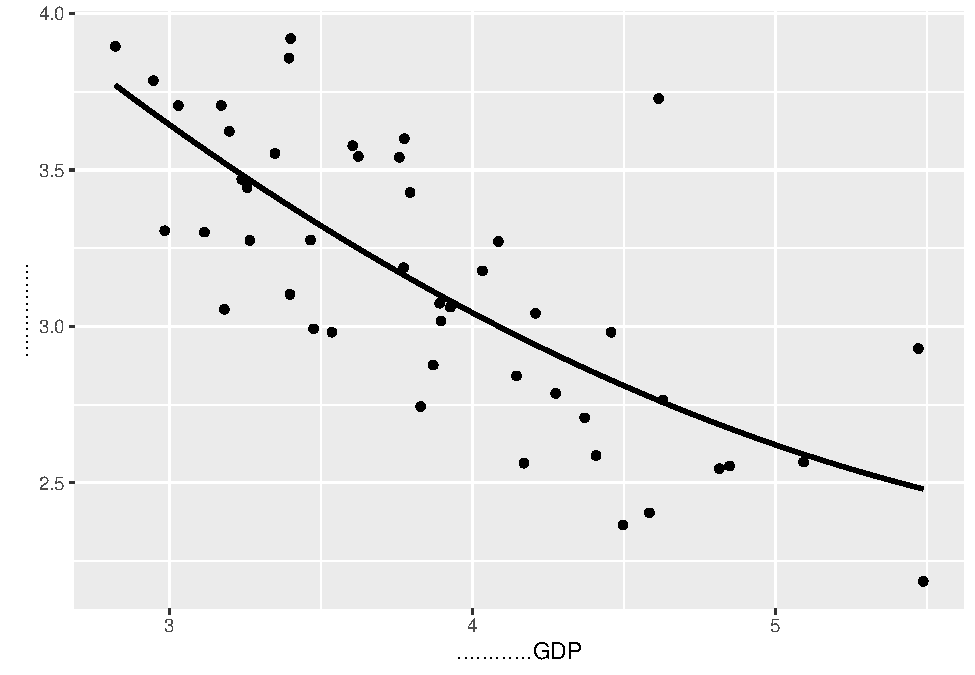
\includegraphics{_main_files/figure-latex/unnamed-chunk-29-1.pdf}

\hypertarget{ux4f8bux984c5.5}{%
\section*{例題5.5}\label{ux4f8bux984c5.5}}
\addcontentsline{toc}{section}{例題5.5}

\begin{Shaded}
\begin{Highlighting}[]
\FunctionTok{lm\_robust}\NormalTok{(growthrate8099 }\SpecialCharTok{\textasciitilde{}}\NormalTok{ lny80 }\SpecialCharTok{*}\NormalTok{ education80, }\AttributeTok{data =}\NormalTok{ youdou, }\AttributeTok{se\_type =} \StringTok{"stata"}\NormalTok{) }\SpecialCharTok{\%\textgreater{}\%} \FunctionTok{summary}\NormalTok{()}
\DocumentationTok{\#\# }
\DocumentationTok{\#\# Call:}
\DocumentationTok{\#\# lm\_robust(formula = growthrate8099 \textasciitilde{} lny80 * education80, data = youdou, }
\DocumentationTok{\#\#     se\_type = "stata")}
\DocumentationTok{\#\# }
\DocumentationTok{\#\# Standard error type:  HC1 }
\DocumentationTok{\#\# }
\DocumentationTok{\#\# Coefficients:}
\DocumentationTok{\#\#                   Estimate Std. Error  t value  Pr(\textgreater{}|t|) CI Lower CI Upper DF}
\DocumentationTok{\#\# (Intercept)         6.0868     1.1220  5.42485 2.492e{-}06    3.824   8.3496 43}
\DocumentationTok{\#\# lny80              {-}2.3937     0.8477 {-}2.82364 7.167e{-}03   {-}4.103  {-}0.6841 43}
\DocumentationTok{\#\# education80         2.5735    11.0413  0.23308 8.168e{-}01  {-}19.693  24.8405 43}
\DocumentationTok{\#\# lny80:education80  {-}0.1211     7.1314 {-}0.01698 9.865e{-}01  {-}14.503  14.2608 43}
\DocumentationTok{\#\# }
\DocumentationTok{\#\# Multiple R{-}squared:  0.561 , Adjusted R{-}squared:  0.5304 }
\DocumentationTok{\#\# F{-}statistic: 18.45 on 3 and 43 DF,  p{-}value: 7.651e{-}08}
\end{Highlighting}
\end{Shaded}

\hypertarget{ux5b9fux8a3cux4f8b5.6-ux90fdux5e02ux5316ux306eux5ea6ux5408ux3044ux3068ux521dux671fux6642ux70b9gdpux306eux4ea4ux4e92ux4f5cux7528}{%
\section*{実証例5.6 都市化の度合いと初期時点GDPの交互作用}\label{ux5b9fux8a3cux4f8b5.6-ux90fdux5e02ux5316ux306eux5ea6ux5408ux3044ux3068ux521dux671fux6642ux70b9gdpux306eux4ea4ux4e92ux4f5cux7528}}
\addcontentsline{toc}{section}{実証例5.6 都市化の度合いと初期時点GDPの交互作用}

先にダミー変数\texttt{urban}を作成してから回帰分析を実行する(下では\texttt{urban}の型は\texttt{int}ではなく\texttt{bool}になるが構わない). \texttt{urban}の値により標本を分ける場合は, \texttt{lm()}の\texttt{data}で\texttt{filter()}を使えばよい.

\begin{Shaded}
\begin{Highlighting}[]
\NormalTok{youdou }\OtherTok{\textless{}{-}}\NormalTok{ youdou }\SpecialCharTok{\%\textgreater{}\%}
    \FunctionTok{mutate}\NormalTok{(}\AttributeTok{urban =}\NormalTok{ did }\SpecialCharTok{\textgreater{}} \FloatTok{0.4}\NormalTok{)}
\FunctionTok{lm}\NormalTok{(growthrate8099 }\SpecialCharTok{\textasciitilde{}}\NormalTok{ urban }\SpecialCharTok{*}\NormalTok{ lny80, }\AttributeTok{data =}\NormalTok{ youdou) }\SpecialCharTok{\%\textgreater{}\%} \FunctionTok{summary}\NormalTok{()}
\DocumentationTok{\#\# }
\DocumentationTok{\#\# Call:}
\DocumentationTok{\#\# lm(formula = growthrate8099 \textasciitilde{} urban * lny80, data = youdou)}
\DocumentationTok{\#\# }
\DocumentationTok{\#\# Residuals:}
\DocumentationTok{\#\#      Min       1Q   Median       3Q      Max }
\DocumentationTok{\#\# {-}0.51040 {-}0.21003 {-}0.02406  0.16516  0.90189 }
\DocumentationTok{\#\# }
\DocumentationTok{\#\# Coefficients:}
\DocumentationTok{\#\#                 Estimate Std. Error t value Pr(\textgreater{}|t|)    }
\DocumentationTok{\#\# (Intercept)      5.74905    0.57763   9.953 9.96e{-}13 ***}
\DocumentationTok{\#\# urbanTRUE       {-}0.17551    0.82444  {-}0.213 0.832421    }
\DocumentationTok{\#\# lny80           {-}1.91120    0.45104  {-}4.237 0.000117 ***}
\DocumentationTok{\#\# urbanTRUE:lny80  0.06441    0.61108   0.105 0.916546    }
\DocumentationTok{\#\# {-}{-}{-}}
\DocumentationTok{\#\# Signif. codes:  0 \textquotesingle{}***\textquotesingle{} 0.001 \textquotesingle{}**\textquotesingle{} 0.01 \textquotesingle{}*\textquotesingle{} 0.05 \textquotesingle{}.\textquotesingle{} 0.1 \textquotesingle{} \textquotesingle{} 1}
\DocumentationTok{\#\# }
\DocumentationTok{\#\# Residual standard error: 0.3092 on 43 degrees of freedom}
\DocumentationTok{\#\# Multiple R{-}squared:  0.5564, Adjusted R{-}squared:  0.5254 }
\DocumentationTok{\#\# F{-}statistic: 17.98 on 3 and 43 DF,  p{-}value: 1.041e{-}07}
\FunctionTok{lm}\NormalTok{(growthrate8099 }\SpecialCharTok{\textasciitilde{}}\NormalTok{ lny80, }\AttributeTok{data =}\NormalTok{ (youdou }\SpecialCharTok{\%\textgreater{}\%} \FunctionTok{filter}\NormalTok{(}\SpecialCharTok{!}\NormalTok{urban))) }\SpecialCharTok{\%\textgreater{}\%} \FunctionTok{summary}\NormalTok{()}
\DocumentationTok{\#\# }
\DocumentationTok{\#\# Call:}
\DocumentationTok{\#\# lm(formula = growthrate8099 \textasciitilde{} lny80, data = (youdou \%\textgreater{}\% filter(!urban)))}
\DocumentationTok{\#\# }
\DocumentationTok{\#\# Residuals:}
\DocumentationTok{\#\#      Min       1Q   Median       3Q      Max }
\DocumentationTok{\#\# {-}0.51040 {-}0.22240 {-}0.02406  0.12827  0.90189 }
\DocumentationTok{\#\# }
\DocumentationTok{\#\# Coefficients:}
\DocumentationTok{\#\#             Estimate Std. Error t value Pr(\textgreater{}|t|)    }
\DocumentationTok{\#\# (Intercept)   5.7491     0.6512   8.829 7.59e{-}09 ***}
\DocumentationTok{\#\# lny80        {-}1.9112     0.5085  {-}3.759  0.00102 ** }
\DocumentationTok{\#\# {-}{-}{-}}
\DocumentationTok{\#\# Signif. codes:  0 \textquotesingle{}***\textquotesingle{} 0.001 \textquotesingle{}**\textquotesingle{} 0.01 \textquotesingle{}*\textquotesingle{} 0.05 \textquotesingle{}.\textquotesingle{} 0.1 \textquotesingle{} \textquotesingle{} 1}
\DocumentationTok{\#\# }
\DocumentationTok{\#\# Residual standard error: 0.3486 on 23 degrees of freedom}
\DocumentationTok{\#\# Multiple R{-}squared:  0.3805, Adjusted R{-}squared:  0.3536 }
\DocumentationTok{\#\# F{-}statistic: 14.13 on 1 and 23 DF,  p{-}value: 0.001022}
\FunctionTok{lm}\NormalTok{(growthrate8099 }\SpecialCharTok{\textasciitilde{}}\NormalTok{ lny80, }\AttributeTok{data =}\NormalTok{ (youdou }\SpecialCharTok{\%\textgreater{}\%} \FunctionTok{filter}\NormalTok{(urban))) }\SpecialCharTok{\%\textgreater{}\%} \FunctionTok{summary}\NormalTok{()}
\DocumentationTok{\#\# }
\DocumentationTok{\#\# Call:}
\DocumentationTok{\#\# lm(formula = growthrate8099 \textasciitilde{} lny80, data = (youdou \%\textgreater{}\% filter(urban)))}
\DocumentationTok{\#\# }
\DocumentationTok{\#\# Residuals:}
\DocumentationTok{\#\#      Min       1Q   Median       3Q      Max }
\DocumentationTok{\#\# {-}0.35740 {-}0.19171 {-}0.05236  0.17634  0.49475 }
\DocumentationTok{\#\# }
\DocumentationTok{\#\# Coefficients:}
\DocumentationTok{\#\#             Estimate Std. Error t value Pr(\textgreater{}|t|)    }
\DocumentationTok{\#\# (Intercept)   5.5735     0.4881  11.419 3.25e{-}10 ***}
\DocumentationTok{\#\# lny80        {-}1.8468     0.3421  {-}5.399 2.77e{-}05 ***}
\DocumentationTok{\#\# {-}{-}{-}}
\DocumentationTok{\#\# Signif. codes:  0 \textquotesingle{}***\textquotesingle{} 0.001 \textquotesingle{}**\textquotesingle{} 0.01 \textquotesingle{}*\textquotesingle{} 0.05 \textquotesingle{}.\textquotesingle{} 0.1 \textquotesingle{} \textquotesingle{} 1}
\DocumentationTok{\#\# }
\DocumentationTok{\#\# Residual standard error: 0.2565 on 20 degrees of freedom}
\DocumentationTok{\#\# Multiple R{-}squared:  0.593,  Adjusted R{-}squared:  0.5727 }
\DocumentationTok{\#\# F{-}statistic: 29.14 on 1 and 20 DF,  p{-}value: 2.769e{-}05}
\end{Highlighting}
\end{Shaded}

\hypertarget{ux5b9fux8a3cux4f8b5.7-ux90fdux5e02ux5316ux306eux5ea6ux5408ux3044ux3068ux521dux671fux6642ux70b9gdpux306eux30c0ux30dfux30fcux5909ux6570ux540cux58ebux306eux4ea4ux4e92ux4f5cux7528}{%
\section*{実証例5.7 都市化の度合いと初期時点GDPのダミー変数同士の交互作用}\label{ux5b9fux8a3cux4f8b5.7-ux90fdux5e02ux5316ux306eux5ea6ux5408ux3044ux3068ux521dux671fux6642ux70b9gdpux306eux30c0ux30dfux30fcux5909ux6570ux540cux58ebux306eux4ea4ux4e92ux4f5cux7528}}
\addcontentsline{toc}{section}{実証例5.7 都市化の度合いと初期時点GDPのダミー変数同士の交互作用}

やはり, 先にダミー変数\texttt{lny80d}を作成する.

\begin{Shaded}
\begin{Highlighting}[]
\NormalTok{youdou }\OtherTok{\textless{}{-}}\NormalTok{ youdou }\SpecialCharTok{\%\textgreater{}\%}
    \FunctionTok{mutate}\NormalTok{(}\AttributeTok{lny80d =}\NormalTok{ lny80 }\SpecialCharTok{\textgreater{}} \FloatTok{1.4}\NormalTok{)}
\FunctionTok{lm}\NormalTok{(growthrate8099 }\SpecialCharTok{\textasciitilde{}}\NormalTok{ urban }\SpecialCharTok{*}\NormalTok{ lny80d, }\AttributeTok{data =}\NormalTok{ youdou) }\SpecialCharTok{\%\textgreater{}\%} \FunctionTok{summary}\NormalTok{()}
\DocumentationTok{\#\# }
\DocumentationTok{\#\# Call:}
\DocumentationTok{\#\# lm(formula = growthrate8099 \textasciitilde{} urban * lny80d, data = youdou)}
\DocumentationTok{\#\# }
\DocumentationTok{\#\# Residuals:}
\DocumentationTok{\#\#      Min       1Q   Median       3Q      Max }
\DocumentationTok{\#\# {-}0.50919 {-}0.25376 {-}0.01148  0.24475  0.85353 }
\DocumentationTok{\#\# }
\DocumentationTok{\#\# Coefficients:}
\DocumentationTok{\#\#                      Estimate Std. Error t value Pr(\textgreater{}|t|)    }
\DocumentationTok{\#\# (Intercept)           3.45474    0.07544  45.793  \textless{} 2e{-}16 ***}
\DocumentationTok{\#\# urbanTRUE            {-}0.23329    0.12459  {-}1.872 0.067953 .  }
\DocumentationTok{\#\# lny80dTRUE           {-}0.58003    0.15400  {-}3.767 0.000498 ***}
\DocumentationTok{\#\# urbanTRUE:lny80dTRUE  0.04725    0.20827   0.227 0.821596    }
\DocumentationTok{\#\# {-}{-}{-}}
\DocumentationTok{\#\# Signif. codes:  0 \textquotesingle{}***\textquotesingle{} 0.001 \textquotesingle{}**\textquotesingle{} 0.01 \textquotesingle{}*\textquotesingle{} 0.05 \textquotesingle{}.\textquotesingle{} 0.1 \textquotesingle{} \textquotesingle{} 1}
\DocumentationTok{\#\# }
\DocumentationTok{\#\# Residual standard error: 0.3288 on 43 degrees of freedom}
\DocumentationTok{\#\# Multiple R{-}squared:  0.4982, Adjusted R{-}squared:  0.4631 }
\DocumentationTok{\#\# F{-}statistic: 14.23 on 3 and 43 DF,  p{-}value: 1.401e{-}06}
\end{Highlighting}
\end{Shaded}

\hypertarget{ux5b9fux8a3cux4f8b5.8-ux975eux7ddaux5f62ux30e2ux30c7ux30ebux306bux304aux3051ux308bux7d50ux5408ux4eeeux8aacux306eux691cux5b9a}{%
\section*{実証例5.8 非線形モデルにおける結合仮説の検定}\label{ux5b9fux8a3cux4f8b5.8-ux975eux7ddaux5f62ux30e2ux30c7ux30ebux306bux304aux3051ux308bux7d50ux5408ux4eeeux8aacux306eux691cux5b9a}}
\addcontentsline{toc}{section}{実証例5.8 非線形モデルにおける結合仮説の検定}

\protect\hyperlink{ex5.5}{実証例5.5}を参照せよ.

\hypertarget{ux5b9fux8a3cux4f8b5.9-ux30ddux30f3ux30d5ux30a7ux30edux30fcux30cbux691cux5b9a}{%
\section*{実証例5.9 ポンフェローニ検定}\label{ux5b9fux8a3cux4f8b5.9-ux30ddux30f3ux30d5ux30a7ux30edux30fcux30cbux691cux5b9a}}
\addcontentsline{toc}{section}{実証例5.9 ポンフェローニ検定}

式は\protect\hyperlink{ex5.1}{実証例5.1}を参照せよ. 規範と教育水準の係数が両方とも0であるという帰無仮説を検定する. F検定統計値は\texttt{car::linearHypothesis()}を使うことで求められる.

\begin{Shaded}
\begin{Highlighting}[]
\FunctionTok{linearHypothesis}\NormalTok{(youdou\_55\_2, }\FunctionTok{c}\NormalTok{(}\StringTok{"norm80"}\NormalTok{,}\StringTok{"education80"}\NormalTok{), }\AttributeTok{test =} \StringTok{"F"}\NormalTok{)}
\DocumentationTok{\#\# Linear hypothesis test}
\DocumentationTok{\#\# }
\DocumentationTok{\#\# Hypothesis:}
\DocumentationTok{\#\# norm80 = 0}
\DocumentationTok{\#\# education80 = 0}
\DocumentationTok{\#\# }
\DocumentationTok{\#\# Model 1: restricted model}
\DocumentationTok{\#\# Model 2: growthrate8099 \textasciitilde{} norm80 + education80 + lny80}
\DocumentationTok{\#\# }
\DocumentationTok{\#\#   Res.Df Df      F   Pr(\textgreater{}F)   }
\DocumentationTok{\#\# 1     45                      }
\DocumentationTok{\#\# 2     43  2 5.4375 0.007848 **}
\DocumentationTok{\#\# {-}{-}{-}}
\DocumentationTok{\#\# Signif. codes:  0 \textquotesingle{}***\textquotesingle{} 0.001 \textquotesingle{}**\textquotesingle{} 0.01 \textquotesingle{}*\textquotesingle{} 0.05 \textquotesingle{}.\textquotesingle{} 0.1 \textquotesingle{} \textquotesingle{} 1}
\end{Highlighting}
\end{Shaded}

\hypertarget{ux88685-5-ux8a18ux8ff0ux7d71ux8a08ux91cf}{%
\section*{表5-5 記述統計量}\label{ux88685-5-ux8a18ux8ff0ux7d71ux8a08ux91cf}}
\addcontentsline{toc}{section}{表5-5 記述統計量}

\texttt{modelsummary::datasummary()}を使うことで簡単に記述統計表が作成できる. ここでは統計量と変数名の表示を日本語に直すため, 一旦dataframeで書き出し, 再度\texttt{gt}で修正した表を表示している.

\begin{Shaded}
\begin{Highlighting}[]
\CommentTok{\# 変数を選択}
\NormalTok{vars }\OtherTok{\textless{}{-}}\NormalTok{ youdou }\SpecialCharTok{\%\textgreater{}\%}
    \FunctionTok{select}\NormalTok{(growthrate8099, trust80, norm80, education80, lny80)}
\NormalTok{table55 }\OtherTok{\textless{}{-}} \FunctionTok{datasummary}\NormalTok{(}\FunctionTok{All}\NormalTok{(vars) }\SpecialCharTok{\textasciitilde{}}\NormalTok{ N }\SpecialCharTok{+}\NormalTok{ Mean }\SpecialCharTok{+}\NormalTok{ SD }\SpecialCharTok{+}\NormalTok{ Min }\SpecialCharTok{+}\NormalTok{ Max,}
            \AttributeTok{data =}\NormalTok{ youdou,}
            \AttributeTok{output =} \StringTok{"data.frame"}\NormalTok{,}
            \AttributeTok{fmt =} \DecValTok{3}\NormalTok{)}
\CommentTok{\# 列名}
\FunctionTok{colnames}\NormalTok{(table55) }\OtherTok{\textless{}{-}} \FunctionTok{c}\NormalTok{(}\StringTok{"変数"}\NormalTok{, }\StringTok{"サンプルサイズ"}\NormalTok{, }\StringTok{"平均"}\NormalTok{, }\StringTok{"標準偏差"}\NormalTok{, }\StringTok{"最小値"}\NormalTok{, }\StringTok{"最大値"}\NormalTok{)}
\CommentTok{\# 変数名}
\NormalTok{table55[,}\DecValTok{1}\NormalTok{] }\OtherTok{\textless{}{-}} \FunctionTok{c}\NormalTok{(}\StringTok{"経済成長率"}\NormalTok{, }\StringTok{"信頼"}\NormalTok{, }\StringTok{"規範"}\NormalTok{, }\StringTok{"教育水準"}\NormalTok{, }\StringTok{"初期時点対数GDP"}\NormalTok{)}
\CommentTok{\# 表を出力}
\FunctionTok{gt}\NormalTok{(table55)}
\end{Highlighting}
\end{Shaded}

\begin{longtable}{lrrrrr}
\toprule
変数 & サンプルサイズ & 平均 & 標準偏差 & 最小値 & 最大値 \\ 
\midrule\addlinespace[2.5pt]
経済成長率 & 47 & 3.147 & 0.449 & 2.185 & 3.920 \\ 
信頼 & 47 & 0.033 & 0.845 & -1.668 & 1.918 \\ 
規範 & 47 & 0.101 & 0.542 & -1.248 & 1.297 \\ 
教育水準 & 47 & 0.112 & 0.036 & 0.069 & 0.238 \\ 
初期時点対数GDP & 47 & 1.341 & 0.167 & 1.037 & 1.703 \\ 
\bottomrule
\end{longtable}

\hypertarget{table5-6}{%
\section*{表5-6 推定結果: 被説明変数は経済成長率}\label{table5-6}}
\addcontentsline{toc}{section}{表5-6 推定結果: 被説明変数は経済成長率}

回帰結果の表は\texttt{modelsummary}を使う (\texttt{stargazer}でも可能だが更新が止まっており, \texttt{estimatr}の結果を表示できないなどデメリットがある). \texttt{modelsummary::msummary()}の\texttt{goef\_omit}で表示しない統計量を指定できるが, これは正規表現を使っているため, 自由度修正済み決定係数\(\bar{R}^2\)を表示し, 通常の決定係数\(R^2\)を表示させないためには\texttt{R2\$}とすればよい. F検定統計量の値を表示するにあたっては, \href{https://stackoverflow.com/questions/69582118/extracting-information-from-r-objects-and-importing-it-to-a-modelsummary-table}{このサイト}を参考にした.

\begin{Shaded}
\begin{Highlighting}[]
\NormalTok{models }\OtherTok{\textless{}{-}} \FunctionTok{list}\NormalTok{(}
    \StringTok{"(1)"} \OtherTok{=} \FunctionTok{lm\_robust}\NormalTok{(growthrate8099 }\SpecialCharTok{\textasciitilde{}}\NormalTok{ trust80, }\AttributeTok{data =}\NormalTok{ youdou, }\AttributeTok{se\_type =} \StringTok{"stata"}\NormalTok{),}
    \StringTok{"(2)"} \OtherTok{=} \FunctionTok{lm\_robust}\NormalTok{(growthrate8099 }\SpecialCharTok{\textasciitilde{}}\NormalTok{ norm80, }\AttributeTok{data =}\NormalTok{ youdou, }\AttributeTok{se\_type =} \StringTok{"stata"}\NormalTok{),}
    \StringTok{"(3)"} \OtherTok{=} \FunctionTok{lm\_robust}\NormalTok{(growthrate8099 }\SpecialCharTok{\textasciitilde{}}\NormalTok{ trust80 }\SpecialCharTok{+}\NormalTok{ norm80, }\AttributeTok{data =}\NormalTok{ youdou, }\AttributeTok{se\_type =} \StringTok{"stata"}\NormalTok{),}
    \StringTok{"(4)"} \OtherTok{=} \FunctionTok{lm\_robust}\NormalTok{(growthrate8099 }\SpecialCharTok{\textasciitilde{}}\NormalTok{ trust80 }\SpecialCharTok{+}\NormalTok{ lny80 }\SpecialCharTok{+}\NormalTok{ education80, }\AttributeTok{data =}\NormalTok{ youdou, }\AttributeTok{se\_type =} \StringTok{"stata"}\NormalTok{),}
    \StringTok{"(5)"} \OtherTok{=} \FunctionTok{lm\_robust}\NormalTok{(growthrate8099 }\SpecialCharTok{\textasciitilde{}}\NormalTok{ norm80 }\SpecialCharTok{+}\NormalTok{ lny80 }\SpecialCharTok{+}\NormalTok{ education80, }\AttributeTok{data =}\NormalTok{ youdou, }\AttributeTok{se\_type =} \StringTok{"stata"}\NormalTok{),}
    \StringTok{"(6)"} \OtherTok{=} \FunctionTok{lm\_robust}\NormalTok{(growthrate8099 }\SpecialCharTok{\textasciitilde{}}\NormalTok{ trust80 }\SpecialCharTok{+}\NormalTok{ norm80 }\SpecialCharTok{+}\NormalTok{ lny80 }\SpecialCharTok{+}\NormalTok{ education80, }\AttributeTok{data =}\NormalTok{ youdou, }\AttributeTok{se\_type =} \StringTok{"stata"}\NormalTok{))}

\CommentTok{\# F検定統計量の値を表示するモデルを指定}
\FunctionTok{attr}\NormalTok{(models[}\DecValTok{3}\NormalTok{]}\SpecialCharTok{$}\StringTok{\textasciigrave{}}\AttributeTok{(3)}\StringTok{\textasciigrave{}}\NormalTok{, }\StringTok{"FTEST"}\NormalTok{) }\OtherTok{\textless{}{-}} \ConstantTok{TRUE}
\FunctionTok{attr}\NormalTok{(models[}\DecValTok{6}\NormalTok{]}\SpecialCharTok{$}\StringTok{\textasciigrave{}}\AttributeTok{(6)}\StringTok{\textasciigrave{}}\NormalTok{, }\StringTok{"FTEST"}\NormalTok{) }\OtherTok{\textless{}{-}} \ConstantTok{TRUE}

\NormalTok{glance\_custom.lm\_robust }\OtherTok{\textless{}{-}} \ControlFlowTok{function}\NormalTok{(x) \{}
    \CommentTok{\# 上で指定した, F検定統計量の値を表示したいモデルでなければパス}
    \ControlFlowTok{if}\NormalTok{ (}\SpecialCharTok{!}\FunctionTok{isTRUE}\NormalTok{(}\FunctionTok{attr}\NormalTok{(x, }\StringTok{"FTEST"}\NormalTok{))) }\FunctionTok{return}\NormalTok{(}\ConstantTok{NULL}\NormalTok{)}

    \CommentTok{\# F検定を実行}
\NormalTok{    ftest }\OtherTok{\textless{}{-}} \FunctionTok{linearHypothesis}\NormalTok{(x, }\AttributeTok{test =} \StringTok{"F"}\NormalTok{, }\FunctionTok{c}\NormalTok{(}\StringTok{"trust80"}\NormalTok{, }\StringTok{"norm80"}\NormalTok{))}

    \CommentTok{\# F検定統計量の値とp値をまとめたtibbleを作成}
\NormalTok{    out }\OtherTok{\textless{}{-}} \FunctionTok{tibble}\NormalTok{(}
        \StringTok{"F検定統計量の値 $H\_0: }\SpecialCharTok{\textbackslash{}\textbackslash{}}\StringTok{beta\_\{信頼\}=0, }\SpecialCharTok{\textbackslash{}\textbackslash{}}\StringTok{beta\_\{規範\}=0$"} \OtherTok{=}\NormalTok{ ftest[[}\StringTok{"F"}\NormalTok{]][}\DecValTok{2}\NormalTok{],}
        \StringTok{"     "} \OtherTok{=} \FunctionTok{sprintf}\NormalTok{(}\StringTok{"(\%.3f)"}\NormalTok{, ftest[[}\StringTok{"Pr(\textgreater{}F)"}\NormalTok{]][}\DecValTok{2}\NormalTok{]))}
    \FunctionTok{return}\NormalTok{(out)}
\NormalTok{\}}

\NormalTok{gm }\OtherTok{\textless{}{-}} \FunctionTok{tribble}\NormalTok{(}
    \SpecialCharTok{\textasciitilde{}}\NormalTok{raw,        }\SpecialCharTok{\textasciitilde{}}\NormalTok{clean,          }\SpecialCharTok{\textasciitilde{}}\NormalTok{fmt,}
    \StringTok{"F検定統計量の値 $H\_0: }\SpecialCharTok{\textbackslash{}\textbackslash{}}\StringTok{beta\_\{信頼\}=0, }\SpecialCharTok{\textbackslash{}\textbackslash{}}\StringTok{beta\_\{規範\}=0$"}\NormalTok{, }\StringTok{"F検定統計量の値 $H\_0: }\SpecialCharTok{\textbackslash{}\textbackslash{}}\StringTok{beta\_\{信頼\}=0, }\SpecialCharTok{\textbackslash{}\textbackslash{}}\StringTok{beta\_\{規範\}=0$"}\NormalTok{, }\DecValTok{3}\NormalTok{,}
    \StringTok{"     "}\NormalTok{, }\StringTok{"     "}\NormalTok{, }\DecValTok{3}\NormalTok{,}
    \StringTok{"adj.r.squared"}\NormalTok{, }\StringTok{"$}\SpecialCharTok{\textbackslash{}\textbackslash{}}\StringTok{bar\{R\}\^{}2$"}\NormalTok{, }\DecValTok{3}\NormalTok{,}
    \StringTok{"nobs"}\NormalTok{, }\StringTok{"サンプルサイズ"}\NormalTok{, }\DecValTok{0}\NormalTok{)}

\FunctionTok{msummary}\NormalTok{(models,}
         \AttributeTok{stars =} \ConstantTok{TRUE}\NormalTok{,}
         \AttributeTok{gof\_omit=}\StringTok{\textquotesingle{}R2$|RMSE|AIC|BIC|Log.Lik.\textquotesingle{}}\NormalTok{,}
         \AttributeTok{gof\_map =}\NormalTok{ gm,}
         \AttributeTok{coef\_map =} \FunctionTok{c}\NormalTok{(}\StringTok{"trust80"} \OtherTok{=} \StringTok{"信頼"}\NormalTok{, }\StringTok{"norm80"} \OtherTok{=} \StringTok{"規範"}\NormalTok{, }\StringTok{"lny80"} \OtherTok{=} \StringTok{"初期時点対数GDP"}\NormalTok{, }\StringTok{"education80"} \OtherTok{=} \StringTok{"教育水準"}\NormalTok{, }\StringTok{"(Intercept)"} \OtherTok{=} \StringTok{"定数項"}\NormalTok{))}
\end{Highlighting}
\end{Shaded}

\begin{table}
\centering
\begin{talltblr}[         %% tabularray outer open
entry=none,label=none,
note{}={+ p < 0.1, * p < 0.05, ** p < 0.01, *** p < 0.001},
]                     %% tabularray outer close
{                     %% tabularray inner open
colspec={Q[]Q[]Q[]Q[]Q[]Q[]Q[]},
column{1}={halign=l,},
column{2}={halign=c,},
column{3}={halign=c,},
column{4}={halign=c,},
column{5}={halign=c,},
column{6}={halign=c,},
column{7}={halign=c,},
hline{12}={1,2,3,4,5,6,7}{solid, 0.05em, black},
}                     %% tabularray inner close
\toprule
& (1) & (2) & (3) & (4) & (5) & (6) \\ \midrule %% TinyTableHeader
信頼                                                                                                    & \num{0.225}**  &                 & \num{0.036}    & \num{0.021}     &                 & \num{-0.012}    \\
& (\num{0.066})  &                 & (\num{0.082})  & (\num{0.076})   &                 & (\num{0.081})   \\
規範                                                                                                    &                 & \num{0.560}*** & \num{0.529}*** &                  & \num{0.338}*   & \num{0.342}*    \\
&                 & (\num{0.071})  & (\num{0.102})  &                  & (\num{0.137})  & (\num{0.148})   \\
初期時点対数GDP                                                                                         &                 &                 &                 & \num{-2.383}*** & \num{-1.991}** & \num{-1.999}*** \\
&                 &                 &                 & (\num{0.491})   & (\num{0.575})  & (\num{0.556})   \\
教育水準                                                                                                &                 &                 &                 & \num{2.612}     & \num{4.387}*   & \num{4.270}+    \\
&                 &                 &                 & (\num{2.709})   & (\num{1.961})  & (\num{2.237})   \\
定数項                                                                                                  & \num{3.139}*** & \num{3.091}*** & \num{3.092}*** & \num{6.049}***  & \num{5.291}*** & \num{5.315}***  \\
& (\num{0.060})  & (\num{0.048})  & (\num{0.048})  & (\num{0.426})   & (\num{0.668})  & (\num{0.603})   \\
F検定統計量の値 \$H\_0: \textbackslash{}beta\_\{信頼\}=0, \textbackslash{}beta\_\{規範\}=0\$ &                 &                 & \num{29.874}   &                  &                 & \num{3.460}     \\
&                 &                 & (0.000)         &                  &                 & (0.041)          \\
\$\textbackslash{}bar\{R\}\textasciicircum{}2\$                                                   & \num{0.161}    & \num{0.444}    & \num{0.435}    & \num{0.531}     & \num{0.614}    & \num{0.605}     \\
サンプルサイズ                                                                                          & \num{47}       & \num{47}       & \num{47}       & \num{47}        & \num{47}       & \num{47}        \\
\bottomrule
\end{talltblr}
\end{table}

F検定統計量の星の表示は, 手動で追加する必要があると思われるので, 一旦省略とする.

\hypertarget{ux88685-7-ux63a8ux5b9aux7d50ux679c}{%
\section*{表5-7 推定結果}\label{ux88685-7-ux63a8ux5b9aux7d50ux679c}}
\addcontentsline{toc}{section}{表5-7 推定結果}

サポートサイトにはデータはないが, Rでは\texttt{wooldridge}パッケージにまとめられているデータ\texttt{attend}を用いることができる.

\begin{Shaded}
\begin{Highlighting}[]
\FunctionTok{data}\NormalTok{(}\StringTok{\textquotesingle{}attend\textquotesingle{}}\NormalTok{)}
\NormalTok{models\_57 }\OtherTok{\textless{}{-}} \FunctionTok{list}\NormalTok{(}
    \StringTok{"(1)"} \OtherTok{=} \FunctionTok{lm\_robust}\NormalTok{(stndfnl }\SpecialCharTok{\textasciitilde{}}\NormalTok{ atndrte }\SpecialCharTok{+}\NormalTok{ frosh }\SpecialCharTok{+}\NormalTok{ soph, }\AttributeTok{data =}\NormalTok{ attend, }\AttributeTok{se\_type =} \StringTok{"stata"}\NormalTok{),}
    \StringTok{"(2)"} \OtherTok{=} \FunctionTok{lm\_robust}\NormalTok{(stndfnl }\SpecialCharTok{\textasciitilde{}}\NormalTok{ atndrte }\SpecialCharTok{+}\NormalTok{ priGPA }\SpecialCharTok{+}\NormalTok{ ACT }\SpecialCharTok{+}\NormalTok{ frosh }\SpecialCharTok{+}\NormalTok{ soph, }\AttributeTok{data =}\NormalTok{ attend, }\AttributeTok{se\_type =} \StringTok{"stata"}\NormalTok{),}
    \StringTok{"(3)"} \OtherTok{=} \FunctionTok{lm\_robust}\NormalTok{(stndfnl }\SpecialCharTok{\textasciitilde{}}\NormalTok{ atndrte }\SpecialCharTok{*}\NormalTok{ priGPA }\SpecialCharTok{+}\NormalTok{ ACT }\SpecialCharTok{+}\NormalTok{ frosh }\SpecialCharTok{+}\NormalTok{ soph, }\AttributeTok{data =}\NormalTok{ attend, }\AttributeTok{se\_type =} \StringTok{"stata"}\NormalTok{),}
    \StringTok{"(4)"} \OtherTok{=} \FunctionTok{lm\_robust}\NormalTok{(stndfnl }\SpecialCharTok{\textasciitilde{}}\NormalTok{ atndrte }\SpecialCharTok{+}\NormalTok{ priGPA }\SpecialCharTok{+} \FunctionTok{I}\NormalTok{(priGPA}\SpecialCharTok{\^{}}\DecValTok{2}\NormalTok{) }\SpecialCharTok{+}\NormalTok{ ACT }\SpecialCharTok{+} \FunctionTok{I}\NormalTok{(ACT}\SpecialCharTok{\^{}}\DecValTok{2}\NormalTok{) }\SpecialCharTok{+}\NormalTok{ frosh }\SpecialCharTok{+}\NormalTok{ soph, }\AttributeTok{data =}\NormalTok{ attend, }\AttributeTok{se\_type =} \StringTok{"stata"}\NormalTok{),}
    \StringTok{"(5)"} \OtherTok{=} \FunctionTok{lm\_robust}\NormalTok{(stndfnl }\SpecialCharTok{\textasciitilde{}}\NormalTok{ atndrte }\SpecialCharTok{*}\NormalTok{ priGPA }\SpecialCharTok{+}\NormalTok{ atndrte }\SpecialCharTok{*} \FunctionTok{I}\NormalTok{(priGPA}\SpecialCharTok{\^{}}\DecValTok{2}\NormalTok{) }\SpecialCharTok{+}\NormalTok{ ACT }\SpecialCharTok{+} \FunctionTok{I}\NormalTok{(ACT}\SpecialCharTok{\^{}}\DecValTok{2}\NormalTok{) }\SpecialCharTok{+}\NormalTok{ frosh }\SpecialCharTok{+}\NormalTok{ soph, }\AttributeTok{data =}\NormalTok{ attend, }\AttributeTok{se\_type =} \StringTok{"stata"}\NormalTok{))}

\NormalTok{cm }\OtherTok{\textless{}{-}} \FunctionTok{c}\NormalTok{(}\StringTok{"atndrte"} \OtherTok{=} \StringTok{"出席割合"}\NormalTok{,}
        \StringTok{"priGPA"} \OtherTok{=} \StringTok{"前学期までのGPA"}\NormalTok{,}
        \StringTok{"I(priGPA\^{}2)"} \OtherTok{=} \StringTok{"前学期までのGPA$\^{}2$"}\NormalTok{,}
        \StringTok{"atndrte:priGPA"} \OtherTok{=} \StringTok{"出席割合 $}\SpecialCharTok{\textbackslash{}\textbackslash{}}\StringTok{times$ 前学期までのGPA"}\NormalTok{,}
        \StringTok{"atndrte:I(priGPA\^{}2)"} \OtherTok{=} \StringTok{"出席割合 $}\SpecialCharTok{\textbackslash{}\textbackslash{}}\StringTok{times$ 前学期までのGPA$\^{}2$"}\NormalTok{,}
        \StringTok{"ACT"} \OtherTok{=} \StringTok{"ACT"}\NormalTok{,}
        \StringTok{"I(ACT\^{}2)"} \OtherTok{=} \StringTok{"ACT$\^{}2$"}\NormalTok{,}
        \StringTok{"frosh"} \OtherTok{=} \StringTok{"1年生"}\NormalTok{,}
        \StringTok{"soph"} \OtherTok{=} \StringTok{"2年生"}\NormalTok{,}
        \StringTok{"(Intercept)"} \OtherTok{=} \StringTok{"定数項"}\NormalTok{)}

\NormalTok{gm }\OtherTok{\textless{}{-}} \FunctionTok{tribble}\NormalTok{(}
    \SpecialCharTok{\textasciitilde{}}\NormalTok{raw,            }\SpecialCharTok{\textasciitilde{}}\NormalTok{clean,           }\SpecialCharTok{\textasciitilde{}}\NormalTok{fmt,}
    \StringTok{"adj.r.squared"}\NormalTok{, }\StringTok{"$}\SpecialCharTok{\textbackslash{}\textbackslash{}}\StringTok{bar\{R\}\^{}2$"}\NormalTok{,   }\DecValTok{2}\NormalTok{,}
    \StringTok{"nobs"}\NormalTok{,          }\StringTok{"サンプルサイズ"}\NormalTok{, }\DecValTok{0}\NormalTok{)}

\CommentTok{\# 丸め関数を定義}
\NormalTok{custom\_format }\OtherTok{\textless{}{-}} \ControlFlowTok{function}\NormalTok{(values) \{}
\NormalTok{    formatted\_values }\OtherTok{\textless{}{-}} \FunctionTok{ifelse}\NormalTok{(values }\SpecialCharTok{\textless{}} \DecValTok{1}\NormalTok{,}
                                \FunctionTok{signif}\NormalTok{(values, }\AttributeTok{digits=}\DecValTok{2}\NormalTok{),}
                                \FunctionTok{round}\NormalTok{(values, }\AttributeTok{digits=}\DecValTok{2}\NormalTok{))}
    \FunctionTok{return}\NormalTok{(formatted\_values)}
\NormalTok{\}}

\CommentTok{\# なぜか定数項だけ丸めがおかしい?}
\FunctionTok{msummary}\NormalTok{(models\_57,}
         \AttributeTok{stars =} \ConstantTok{TRUE}\NormalTok{,}
         \AttributeTok{gof\_omit=}\StringTok{\textquotesingle{}R2$|RMSE|AIC|BIC|Log.Lik.\textquotesingle{}}\NormalTok{,}
         \AttributeTok{coef\_map =}\NormalTok{ cm,}
         \AttributeTok{gof\_map =}\NormalTok{ gm,}
         \AttributeTok{fmt =}\NormalTok{ custom\_format)}
\end{Highlighting}
\end{Shaded}

\begin{table}
\centering
\begin{talltblr}[         %% tabularray outer open
entry=none,label=none,
note{}={+ p < 0.1, * p < 0.05, ** p < 0.01, *** p < 0.001},
]                     %% tabularray outer close
{                     %% tabularray inner open
colspec={Q[]Q[]Q[]Q[]Q[]Q[]},
column{1}={halign=l,},
column{2}={halign=c,},
column{3}={halign=c,},
column{4}={halign=c,},
column{5}={halign=c,},
column{6}={halign=c,},
hline{22}={1,2,3,4,5,6}{solid, 0.05em, black},
}                     %% tabularray inner close
\toprule
& (1) & (2) & (3) & (4) & (5) \\ \midrule %% TinyTableHeader
出席割合                                                                        & \num{0.0082}*** & \num{0.0052}*  & \num{-0.022}*  & \num{0.0062}** & \num{0.065}*   \\
& (\num{0.0021})  & (\num{0.0024}) & (\num{0.0088}) & (\num{0.0023}) & (\num{0.032})  \\
前学期までのGPA                                                                 &                  & \num{0.43}***  & \num{-0.56}+   & \num{-1.5}**   & \num{3.63}     \\
&                  & (\num{0.086})  & (\num{0.32})   & (\num{0.49})   & (\num{2.21})   \\
前学期までのGPA\$\textasciicircum{}2\$                                       &                  &                 &                 & \num{0.37}***  & \num{-0.82}+   \\
&                  &                 &                 & (\num{0.09})   & (\num{0.45})   \\
出席割合 \$\textbackslash{}times\$ 前学期までのGPA                           &                  &                 & \num{0.012}**  &                 & \num{-0.057}*  \\
&                  &                 & (\num{0.0037}) &                 & (\num{0.026})  \\
出席割合 \$\textbackslash{}times\$ 前学期までのGPA\$\textasciicircum{}2\$ &                  &                 &                 &                 & \num{0.013}*   \\
&                  &                 &                 &                 & (\num{0.0052}) \\
ACT                                                                             &                  & \num{0.084}*** & \num{0.082}*** & \num{-0.11}    & \num{-0.11}    \\
&                  & (\num{0.011})  & (\num{0.011})  & (\num{0.1})    & (\num{0.1})    \\
ACT\$\textasciicircum{}2\$                                                   &                  &                 &                 & \num{0.0042}+  & \num{0.0042}+  \\
&                  &                 &                 & (\num{0.0023}) & (\num{0.0022}) \\
1年生                                                                           & \num{-0.29}*    & \num{-0.049}   & \num{-0.063}   & \num{-0.11}    & \num{-0.1}     \\
& (\num{0.11})    & (\num{0.11})   & (\num{0.1})    & (\num{0.1})    & (\num{0.1})    \\
2年生                                                                           & \num{-0.12}     & \num{-0.16}+   & \num{-0.17}+   & \num{-0.18}*   & \num{-0.19}*   \\
& (\num{0.1})     & (\num{0.089})  & (\num{0.088})  & (\num{0.087})  & (\num{0.086})  \\
定数項                                                                          & \num{-0.5}**    & \num{-3.3}***  & \num{-1}       & \num{1.38}     & \num{-3.9}     \\
& (\num{0.18})    & (\num{0.3})    & (\num{0.76})   & (\num{1.24})   & (\num{2.95})   \\
\$\textbackslash{}bar\{R\}\textasciicircum{}2\$                           & \num{0.02}      & \num{0.20}     & \num{0.21}     & \num{0.22}     & \num{0.23}     \\
サンプルサイズ                                                                  & \num{680}       & \num{680}      & \num{680}      & \num{680}      & \num{680}      \\
\bottomrule
\end{talltblr}
\end{table}

F検定統計量の表への記載は省略とし, 下に検定結果を示す.

\begin{Shaded}
\begin{Highlighting}[]
\FunctionTok{linearHypothesis}\NormalTok{(models\_57[}\DecValTok{3}\NormalTok{]}\SpecialCharTok{$}\StringTok{\textasciigrave{}}\AttributeTok{(3)}\StringTok{\textasciigrave{}}\NormalTok{, }\AttributeTok{test =} \StringTok{"F"}\NormalTok{, }\FunctionTok{c}\NormalTok{(}\StringTok{"atndrte"}\NormalTok{, }\StringTok{"atndrte:priGPA"}\NormalTok{))}
\DocumentationTok{\#\# Linear hypothesis test}
\DocumentationTok{\#\# }
\DocumentationTok{\#\# Hypothesis:}
\DocumentationTok{\#\# atndrte = 0}
\DocumentationTok{\#\# atndrte:priGPA = 0}
\DocumentationTok{\#\# }
\DocumentationTok{\#\# Model 1: restricted model}
\DocumentationTok{\#\# Model 2: stndfnl \textasciitilde{} atndrte * priGPA + ACT + frosh + soph}
\DocumentationTok{\#\# }
\DocumentationTok{\#\#   Res.Df Df      F    Pr(\textgreater{}F)    }
\DocumentationTok{\#\# 1    675                        }
\DocumentationTok{\#\# 2    673  2 7.8085 0.0004442 ***}
\DocumentationTok{\#\# {-}{-}{-}}
\DocumentationTok{\#\# Signif. codes:  0 \textquotesingle{}***\textquotesingle{} 0.001 \textquotesingle{}**\textquotesingle{} 0.01 \textquotesingle{}*\textquotesingle{} 0.05 \textquotesingle{}.\textquotesingle{} 0.1 \textquotesingle{} \textquotesingle{} 1}
\FunctionTok{linearHypothesis}\NormalTok{(models\_57[}\DecValTok{4}\NormalTok{]}\SpecialCharTok{$}\StringTok{\textasciigrave{}}\AttributeTok{(4)}\StringTok{\textasciigrave{}}\NormalTok{, }\AttributeTok{test =} \StringTok{"F"}\NormalTok{, }\FunctionTok{c}\NormalTok{(}\StringTok{"I(priGPA\^{}2)"}\NormalTok{, }\StringTok{"I(ACT\^{}2)"}\NormalTok{))}
\DocumentationTok{\#\# Linear hypothesis test}
\DocumentationTok{\#\# }
\DocumentationTok{\#\# Hypothesis:}
\DocumentationTok{\#\# I(priGPA\^{}2) = 0}
\DocumentationTok{\#\# I(ACT\^{}2) = 0}
\DocumentationTok{\#\# }
\DocumentationTok{\#\# Model 1: restricted model}
\DocumentationTok{\#\# Model 2: stndfnl \textasciitilde{} atndrte + priGPA + I(priGPA\^{}2) + ACT + I(ACT\^{}2) + frosh + }
\DocumentationTok{\#\#     soph}
\DocumentationTok{\#\# }
\DocumentationTok{\#\#   Res.Df Df      F    Pr(\textgreater{}F)    }
\DocumentationTok{\#\# 1    674                        }
\DocumentationTok{\#\# 2    672  2 11.772 9.438e{-}06 ***}
\DocumentationTok{\#\# {-}{-}{-}}
\DocumentationTok{\#\# Signif. codes:  0 \textquotesingle{}***\textquotesingle{} 0.001 \textquotesingle{}**\textquotesingle{} 0.01 \textquotesingle{}*\textquotesingle{} 0.05 \textquotesingle{}.\textquotesingle{} 0.1 \textquotesingle{} \textquotesingle{} 1}
\FunctionTok{linearHypothesis}\NormalTok{(models\_57[}\DecValTok{5}\NormalTok{]}\SpecialCharTok{$}\StringTok{\textasciigrave{}}\AttributeTok{(5)}\StringTok{\textasciigrave{}}\NormalTok{, }\AttributeTok{test =} \StringTok{"F"}\NormalTok{, }\FunctionTok{c}\NormalTok{(}\StringTok{"atndrte"}\NormalTok{, }\StringTok{"atndrte:priGPA"}\NormalTok{, }\StringTok{"atndrte:I(priGPA\^{}2)"}\NormalTok{))}
\DocumentationTok{\#\# Linear hypothesis test}
\DocumentationTok{\#\# }
\DocumentationTok{\#\# Hypothesis:}
\DocumentationTok{\#\# atndrte = 0}
\DocumentationTok{\#\# atndrte:priGPA = 0}
\DocumentationTok{\#\# atndrte:I(priGPA\^{}2) = 0}
\DocumentationTok{\#\# }
\DocumentationTok{\#\# Model 1: restricted model}
\DocumentationTok{\#\# Model 2: stndfnl \textasciitilde{} atndrte * priGPA + atndrte * I(priGPA\^{}2) + ACT + I(ACT\^{}2) + }
\DocumentationTok{\#\#     frosh + soph}
\DocumentationTok{\#\# }
\DocumentationTok{\#\#   Res.Df Df      F    Pr(\textgreater{}F)    }
\DocumentationTok{\#\# 1    673                        }
\DocumentationTok{\#\# 2    670  3 6.2543 0.0003437 ***}
\DocumentationTok{\#\# {-}{-}{-}}
\DocumentationTok{\#\# Signif. codes:  0 \textquotesingle{}***\textquotesingle{} 0.001 \textquotesingle{}**\textquotesingle{} 0.01 \textquotesingle{}*\textquotesingle{} 0.05 \textquotesingle{}.\textquotesingle{} 0.1 \textquotesingle{} \textquotesingle{} 1}
\FunctionTok{linearHypothesis}\NormalTok{(models\_57[}\DecValTok{5}\NormalTok{]}\SpecialCharTok{$}\StringTok{\textasciigrave{}}\AttributeTok{(5)}\StringTok{\textasciigrave{}}\NormalTok{, }\AttributeTok{test =} \StringTok{"F"}\NormalTok{, }\FunctionTok{c}\NormalTok{(}\StringTok{"I(priGPA\^{}2)"}\NormalTok{, }\StringTok{"atndrte:I(priGPA\^{}2)"}\NormalTok{, }\StringTok{"I(ACT\^{}2)"}\NormalTok{))}
\DocumentationTok{\#\# Linear hypothesis test}
\DocumentationTok{\#\# }
\DocumentationTok{\#\# Hypothesis:}
\DocumentationTok{\#\# I(priGPA\^{}2) = 0}
\DocumentationTok{\#\# atndrte:I(priGPA\^{}2) = 0}
\DocumentationTok{\#\# I(ACT\^{}2) = 0}
\DocumentationTok{\#\# }
\DocumentationTok{\#\# Model 1: restricted model}
\DocumentationTok{\#\# Model 2: stndfnl \textasciitilde{} atndrte * priGPA + atndrte * I(priGPA\^{}2) + ACT + I(ACT\^{}2) + }
\DocumentationTok{\#\#     frosh + soph}
\DocumentationTok{\#\# }
\DocumentationTok{\#\#   Res.Df Df      F    Pr(\textgreater{}F)    }
\DocumentationTok{\#\# 1    673                        }
\DocumentationTok{\#\# 2    670  3 7.5692 5.521e{-}05 ***}
\DocumentationTok{\#\# {-}{-}{-}}
\DocumentationTok{\#\# Signif. codes:  0 \textquotesingle{}***\textquotesingle{} 0.001 \textquotesingle{}**\textquotesingle{} 0.01 \textquotesingle{}*\textquotesingle{} 0.05 \textquotesingle{}.\textquotesingle{} 0.1 \textquotesingle{} \textquotesingle{} 1}
\FunctionTok{linearHypothesis}\NormalTok{(models\_57[}\DecValTok{5}\NormalTok{]}\SpecialCharTok{$}\StringTok{\textasciigrave{}}\AttributeTok{(5)}\StringTok{\textasciigrave{}}\NormalTok{, }\AttributeTok{test =} \StringTok{"F"}\NormalTok{, }\FunctionTok{c}\NormalTok{(}\StringTok{"atndrte:priGPA"}\NormalTok{, }\StringTok{"atndrte:I(priGPA\^{}2)"}\NormalTok{))}
\DocumentationTok{\#\# Linear hypothesis test}
\DocumentationTok{\#\# }
\DocumentationTok{\#\# Hypothesis:}
\DocumentationTok{\#\# atndrte:priGPA = 0}
\DocumentationTok{\#\# atndrte:I(priGPA\^{}2) = 0}
\DocumentationTok{\#\# }
\DocumentationTok{\#\# Model 1: restricted model}
\DocumentationTok{\#\# Model 2: stndfnl \textasciitilde{} atndrte * priGPA + atndrte * I(priGPA\^{}2) + ACT + I(ACT\^{}2) + }
\DocumentationTok{\#\#     frosh + soph}
\DocumentationTok{\#\# }
\DocumentationTok{\#\#   Res.Df Df      F   Pr(\textgreater{}F)   }
\DocumentationTok{\#\# 1    672                      }
\DocumentationTok{\#\# 2    670  2 5.1942 0.005774 **}
\DocumentationTok{\#\# {-}{-}{-}}
\DocumentationTok{\#\# Signif. codes:  0 \textquotesingle{}***\textquotesingle{} 0.001 \textquotesingle{}**\textquotesingle{} 0.01 \textquotesingle{}*\textquotesingle{} 0.05 \textquotesingle{}.\textquotesingle{} 0.1 \textquotesingle{} \textquotesingle{} 1}
\end{Highlighting}
\end{Shaded}

\hypertarget{ux7df4ux7fd2ux554fux984c-5-14-ux5b9fux8a3c}{%
\section*{練習問題 5-14 {[}実証{]}}\label{ux7df4ux7fd2ux554fux984c-5-14-ux5b9fux8a3c}}
\addcontentsline{toc}{section}{練習問題 5-14 {[}実証{]}}

\begin{enumerate}
\def\labelenumi{\alph{enumi}.}
\item
  表5-6を参照せよ.
\item
  自由度修正済み決定係数\(\bar{R}^2\)は以下のように定義される (p.158).
\end{enumerate}

\[\bar{R}^2 = 1 - \frac{N-1}{N-k-1}\frac{\sum_{i=1}^N\hat{u}_i^2}{\sum_{i=1}^N(Y_i-\bar{Y}^2)}\].

これを決定係数\(R^2\)の定義と比べると, 自由度修正済み決定係数は変数の数\(k\)が増えるたびに値が小さくなることがわかる. 決定係数\(R^2\)ではこのようなことは起きず, 変数の数を増やすと\(R^2\)の値は必ず変わらないか大きくなり, 小さくなることはない.

\begin{enumerate}
\def\labelenumi{\alph{enumi}.}
\setcounter{enumi}{2}
\tightlist
\item
  問題文の指示の通り回帰分析を実行する. 1つめの方法では標準偏差の値は一致しないが, 2つ目の方法では一致することが確認できる.
\end{enumerate}

\begin{Shaded}
\begin{Highlighting}[]
\NormalTok{practice514c\_1 }\OtherTok{\textless{}{-}} \FunctionTok{lm}\NormalTok{(trust80 }\SpecialCharTok{\textasciitilde{}}\NormalTok{ norm80, }\AttributeTok{data =}\NormalTok{ youdou)}
\NormalTok{practice514c\_2 }\OtherTok{\textless{}{-}} \FunctionTok{lm\_robust}\NormalTok{(growthrate8099 }\SpecialCharTok{\textasciitilde{}} \DecValTok{0} \SpecialCharTok{+}\NormalTok{ practice514c\_1}\SpecialCharTok{$}\NormalTok{residuals, }\AttributeTok{data =}\NormalTok{ youdou, }\AttributeTok{se\_type =} \StringTok{"stata"}\NormalTok{)}
\FunctionTok{summary}\NormalTok{(practice514c\_2)}\SpecialCharTok{$}\NormalTok{coefficients}
\DocumentationTok{\#\#                           Estimate Std. Error    t value  Pr(\textgreater{}|t|)  CI Lower}
\DocumentationTok{\#\# practice514c\_1$residuals 0.0358709  0.7030377 0.05102272 0.9595283 {-}1.379271}
\DocumentationTok{\#\#                          CI Upper DF}
\DocumentationTok{\#\# practice514c\_1$residuals 1.451012 46}

\NormalTok{practice514c\_3 }\OtherTok{\textless{}{-}} \FunctionTok{lm}\NormalTok{(growthrate8099 }\SpecialCharTok{\textasciitilde{}}\NormalTok{ norm80, }\AttributeTok{data =}\NormalTok{ youdou)}
\NormalTok{practice514c\_4 }\OtherTok{\textless{}{-}} \FunctionTok{lm}\NormalTok{(trust80 }\SpecialCharTok{\textasciitilde{}} \DecValTok{0} \SpecialCharTok{+}\NormalTok{ norm80, }\AttributeTok{data =}\NormalTok{ youdou)}
\NormalTok{practice514c\_5 }\OtherTok{\textless{}{-}} \FunctionTok{lm\_robust}\NormalTok{(practice514c\_3}\SpecialCharTok{$}\NormalTok{residuals }\SpecialCharTok{\textasciitilde{}} \DecValTok{0} \SpecialCharTok{+}\NormalTok{ practice514c\_4}\SpecialCharTok{$}\NormalTok{residuals, }\AttributeTok{se\_type =} \StringTok{"stata"}\NormalTok{)}
\FunctionTok{summary}\NormalTok{(practice514c\_5)}\SpecialCharTok{$}\NormalTok{coefficients}
\DocumentationTok{\#\#                            Estimate Std. Error   t value  Pr(\textgreater{}|t|)   CI Lower}
\DocumentationTok{\#\# practice514c\_4$residuals 0.03566014 0.08075573 0.4415803 0.6608618 {-}0.1268927}
\DocumentationTok{\#\#                          CI Upper DF}
\DocumentationTok{\#\# practice514c\_4$residuals 0.198213 46}
\end{Highlighting}
\end{Shaded}

\hypertarget{ux7df4ux7fd2ux554fux984c-5-15-ux5b9fux8a3c}{%
\section*{練習問題 5-15 {[}実証{]}}\label{ux7df4ux7fd2ux554fux984c-5-15-ux5b9fux8a3c}}
\addcontentsline{toc}{section}{練習問題 5-15 {[}実証{]}}

データはStataで用いられる\texttt{.dta}形式になっているが, これをRで読み込むには\texttt{haven::read\_dta()}を使う.

\begin{Shaded}
\begin{Highlighting}[]
\NormalTok{timss }\OtherTok{\textless{}{-}} \FunctionTok{read\_dta}\NormalTok{(}\StringTok{"data/05\_第5章/timss.dta"}\NormalTok{)}

\NormalTok{practice5\_15\_a }\OtherTok{\textless{}{-}} \FunctionTok{lm\_robust}\NormalTok{(mathscore }\SpecialCharTok{\textasciitilde{}}\NormalTok{ agese\_q2 }\SpecialCharTok{+}\NormalTok{ agese\_q3 }\SpecialCharTok{+}\NormalTok{ agese\_q4, }\AttributeTok{data =}\NormalTok{ timss, }\AttributeTok{se\_type =} \StringTok{"stata"}\NormalTok{)}
\NormalTok{practice5\_15\_c }\OtherTok{\textless{}{-}} \FunctionTok{lm\_robust}\NormalTok{(mathscore }\SpecialCharTok{\textasciitilde{}}\NormalTok{ gender}\SpecialCharTok{*}\NormalTok{agese\_q2 }\SpecialCharTok{+}\NormalTok{ gender}\SpecialCharTok{*}\NormalTok{agese\_q3 }\SpecialCharTok{+}\NormalTok{ gender}\SpecialCharTok{*}\NormalTok{agese\_q4, }\AttributeTok{data =}\NormalTok{ timss, }\AttributeTok{se\_type =} \StringTok{"stata"}\NormalTok{)}
\NormalTok{practice5\_15\_d }\OtherTok{\textless{}{-}} \FunctionTok{lm\_robust}\NormalTok{(mathscore }\SpecialCharTok{\textasciitilde{}}\NormalTok{ agese\_q2 }\SpecialCharTok{+}\NormalTok{ agese\_q3 }\SpecialCharTok{+}\NormalTok{ agese\_q4 }\SpecialCharTok{+}\NormalTok{ comu\_1 }\SpecialCharTok{+}\NormalTok{ comu\_2 }\SpecialCharTok{+}\NormalTok{ comu\_3 }\SpecialCharTok{+}\NormalTok{ comu\_4 }\SpecialCharTok{+}\NormalTok{ comu\_5 }\SpecialCharTok{+}\NormalTok{ computer }\SpecialCharTok{+}\NormalTok{ numpeople }\SpecialCharTok{+}\NormalTok{ mothereduc\_1 }\SpecialCharTok{+}\NormalTok{ mothereduc\_2 }\SpecialCharTok{+}\NormalTok{ mothereduc\_3 }\SpecialCharTok{+}\NormalTok{ mothereduc\_4 }\SpecialCharTok{+}\NormalTok{ mothereduc\_5 }\SpecialCharTok{+}\NormalTok{ fathereduc\_1 }\SpecialCharTok{+}\NormalTok{ fathereduc\_2 }\SpecialCharTok{+}\NormalTok{ fathereduc\_3 }\SpecialCharTok{+}\NormalTok{ fathereduc\_4 }\SpecialCharTok{+}\NormalTok{ fathereduc\_5, }\AttributeTok{data =}\NormalTok{ timss, }\AttributeTok{se\_type =} \StringTok{"stata"}\NormalTok{)}
\NormalTok{practice5\_15\_ea }\OtherTok{\textless{}{-}} \FunctionTok{lm\_robust}\NormalTok{(sciencescore }\SpecialCharTok{\textasciitilde{}}\NormalTok{ agese\_q2 }\SpecialCharTok{+}\NormalTok{ agese\_q3 }\SpecialCharTok{+}\NormalTok{ agese\_q4, }\AttributeTok{data =}\NormalTok{ timss, }\AttributeTok{se\_type =} \StringTok{"stata"}\NormalTok{)}
\NormalTok{practice5\_15\_ec }\OtherTok{\textless{}{-}} \FunctionTok{lm\_robust}\NormalTok{(sciencescore }\SpecialCharTok{\textasciitilde{}}\NormalTok{ gender}\SpecialCharTok{*}\NormalTok{agese\_q2 }\SpecialCharTok{+}\NormalTok{ gender}\SpecialCharTok{*}\NormalTok{agese\_q3 }\SpecialCharTok{+}\NormalTok{ gender}\SpecialCharTok{*}\NormalTok{agese\_q4, }\AttributeTok{data =}\NormalTok{ timss, }\AttributeTok{se\_type =} \StringTok{"stata"}\NormalTok{)}
\NormalTok{practice5\_15\_ed }\OtherTok{\textless{}{-}} \FunctionTok{lm\_robust}\NormalTok{(sciencescore }\SpecialCharTok{\textasciitilde{}}\NormalTok{ agese\_q2 }\SpecialCharTok{+}\NormalTok{ agese\_q3 }\SpecialCharTok{+}\NormalTok{ agese\_q4 }\SpecialCharTok{+}\NormalTok{ comu\_1 }\SpecialCharTok{+}\NormalTok{ comu\_2 }\SpecialCharTok{+}\NormalTok{ comu\_3 }\SpecialCharTok{+}\NormalTok{ comu\_4 }\SpecialCharTok{+}\NormalTok{ comu\_5 }\SpecialCharTok{+}\NormalTok{ computer }\SpecialCharTok{+}\NormalTok{ numpeople }\SpecialCharTok{+}\NormalTok{ mothereduc\_1 }\SpecialCharTok{+}\NormalTok{ mothereduc\_2 }\SpecialCharTok{+}\NormalTok{ mothereduc\_3 }\SpecialCharTok{+}\NormalTok{ mothereduc\_4 }\SpecialCharTok{+}\NormalTok{ mothereduc\_5 }\SpecialCharTok{+}\NormalTok{ fathereduc\_1 }\SpecialCharTok{+}\NormalTok{ fathereduc\_2 }\SpecialCharTok{+}\NormalTok{ fathereduc\_3 }\SpecialCharTok{+}\NormalTok{ fathereduc\_4 }\SpecialCharTok{+}\NormalTok{ fathereduc\_5, }\AttributeTok{data =}\NormalTok{ timss, }\AttributeTok{se\_type =} \StringTok{"stata"}\NormalTok{)}
\end{Highlighting}
\end{Shaded}

結果を\texttt{modelsummary}で表にまとめる. (d)で用いるダミー変数は\texttt{coef\_map}で指定して表示を省略している.

\begin{Shaded}
\begin{Highlighting}[]
\NormalTok{models\_5\_15 }\OtherTok{\textless{}{-}} \FunctionTok{list}\NormalTok{()}
\NormalTok{models\_5\_15[[}\StringTok{\textquotesingle{}a\textquotesingle{}}\NormalTok{]] }\OtherTok{\textless{}{-}}\NormalTok{ practice5\_15\_a}
\NormalTok{models\_5\_15[[}\StringTok{\textquotesingle{}c\textquotesingle{}}\NormalTok{]] }\OtherTok{\textless{}{-}}\NormalTok{ practice5\_15\_c}
\NormalTok{models\_5\_15[[}\StringTok{\textquotesingle{}d\textquotesingle{}}\NormalTok{]] }\OtherTok{\textless{}{-}}\NormalTok{ practice5\_15\_d}
\NormalTok{models\_5\_15[[}\StringTok{\textquotesingle{}ea\textquotesingle{}}\NormalTok{]] }\OtherTok{\textless{}{-}}\NormalTok{ practice5\_15\_ea}
\NormalTok{models\_5\_15[[}\StringTok{\textquotesingle{}ec\textquotesingle{}}\NormalTok{]] }\OtherTok{\textless{}{-}}\NormalTok{ practice5\_15\_ec}
\NormalTok{models\_5\_15[[}\StringTok{\textquotesingle{}ed\textquotesingle{}}\NormalTok{]] }\OtherTok{\textless{}{-}}\NormalTok{ practice5\_15\_ed}
\NormalTok{cm }\OtherTok{\textless{}{-}} \FunctionTok{c}\NormalTok{(}\StringTok{"agese\_q2"}\NormalTok{,}
        \StringTok{"agese\_q3"}\NormalTok{,}
        \StringTok{"agese\_q4"}\NormalTok{,}
        \StringTok{"gender"}\NormalTok{,}
        \StringTok{"gender:agese\_q2"}\NormalTok{,}
        \StringTok{"gender:agese\_q3"}\NormalTok{,}
        \StringTok{"gender:agese\_q4"}\NormalTok{,}
        \StringTok{"(Intercept)"}\NormalTok{)}
\NormalTok{gm }\OtherTok{\textless{}{-}} \FunctionTok{tribble}\NormalTok{(}
    \SpecialCharTok{\textasciitilde{}}\NormalTok{raw,            }\SpecialCharTok{\textasciitilde{}}\NormalTok{clean,           }\SpecialCharTok{\textasciitilde{}}\NormalTok{fmt,}
    \StringTok{"adj.r.squared"}\NormalTok{, }\StringTok{"$}\SpecialCharTok{\textbackslash{}\textbackslash{}}\StringTok{bar\{R\}\^{}2$"}\NormalTok{,   }\DecValTok{2}\NormalTok{,}
    \StringTok{"nobs"}\NormalTok{,          }\StringTok{"サンプルサイズ"}\NormalTok{, }\DecValTok{0}\NormalTok{)}
\FunctionTok{msummary}\NormalTok{(models\_5\_15,}
         \AttributeTok{coef\_map =}\NormalTok{ cm,}
         \AttributeTok{gof\_map =}\NormalTok{ gm,}
         \AttributeTok{stars =} \ConstantTok{TRUE}\NormalTok{)}
\end{Highlighting}
\end{Shaded}

\begin{table}
\centering
\begin{talltblr}[         %% tabularray outer open
entry=none,label=none,
note{}={+ p < 0.1, * p < 0.05, ** p < 0.01, *** p < 0.001},
]                     %% tabularray outer close
{                     %% tabularray inner open
colspec={Q[]Q[]Q[]Q[]Q[]Q[]Q[]},
column{1}={halign=l,},
column{2}={halign=c,},
column{3}={halign=c,},
column{4}={halign=c,},
column{5}={halign=c,},
column{6}={halign=c,},
column{7}={halign=c,},
hline{18}={1,2,3,4,5,6,7}{solid, 0.05em, black},
}                     %% tabularray inner close
\toprule
& a & c & d & ea & ec & ed \\ \midrule %% TinyTableHeader
agese\_q2                                            & \num{0.174}      & \num{-0.500}     & \num{0.218}      & \num{0.261}      & \num{0.006}      & \num{0.317}      \\
& (\num{0.412})    & (\num{1.282})    & (\num{0.394})    & (\num{0.420})    & (\num{1.302})    & (\num{0.406})    \\
agese\_q3                                            & \num{-0.346}     & \num{-1.516}     & \num{-0.460}     & \num{-0.543}     & \num{-1.274}     & \num{-0.614}     \\
& (\num{0.415})    & (\num{1.291})    & (\num{0.395})    & (\num{0.419})    & (\num{1.274})    & (\num{0.406})    \\
agese\_q4                                            & \num{-1.558}***  & \num{-2.935}*    & \num{-1.336}***  & \num{-1.717}***  & \num{-1.963}     & \num{-1.522}***  \\
& (\num{0.419})    & (\num{1.289})    & (\num{0.403})    & (\num{0.428})    & (\num{1.312})    & (\num{0.413})    \\
gender                                                &                   & \num{-0.137}     &                   &                   & \num{1.031}+     &                   \\
&                   & (\num{0.586})    &                   &                   & (\num{0.611})    &                   \\
gender:agese\_q2                                     &                   & \num{0.445}      &                   &                   & \num{0.147}      &                   \\
&                   & (\num{0.824})    &                   &                   & (\num{0.840})    &                   \\
gender:agese\_q3                                     &                   & \num{0.783}      &                   &                   & \num{0.487}      &                   \\
&                   & (\num{0.830})    &                   &                   & (\num{0.839})    &                   \\
gender:agese\_q4                                     &                   & \num{0.920}      &                   &                   & \num{0.160}      &                   \\
&                   & (\num{0.839})    &                   &                   & (\num{0.856})    &                   \\
(Intercept)                                           & \num{150.363}*** & \num{150.568}*** & \num{146.798}*** & \num{150.453}*** & \num{148.915}*** & \num{150.811}*** \\
& (\num{0.293})    & (\num{0.908})    & (\num{2.392})    & (\num{0.305})    & (\num{0.923})    & (\num{1.884})    \\
\$\textbackslash{}bar\{R\}\textasciicircum{}2\$ & \num{0.00}       & \num{0.00}       & \num{0.09}       & \num{0.00}       & \num{0.01}       & \num{0.07}       \\
サンプルサイズ                                        & \num{4536}       & \num{4536}       & \num{4536}       & \num{4536}       & \num{4536}       & \num{4536}       \\
\bottomrule
\end{talltblr}
\end{table}

\begin{enumerate}
\def\labelenumi{\alph{enumi}.}
\item
  上の表のa式を見ると, \texttt{agese\_q4}の係数は有意に負であることがわかる. つまり, この結果では早生まれの人の成績は4月から6月に生まれた人に比べて低いといえる.
\item
  生まれた四半期のダミー変数を4つすべて含むと, ダミー変数の罠に陥る. 4月から6月に生まれた人を表すダミー変数を使用する場合, 定数項なしの回帰を行うことでダミー変数の罠を避けられる. 4月から6月に生まれた人, 早生まれの人を表すダミー変数の係数をそれぞれ\(\beta_{Q1}, \beta_{Q4}\)とおくと, 帰無仮説は\(H_0: \beta_{Q4} < \beta_{Q1}\)とすればよい.
\item
  上の表のc式を見ると, \texttt{gender}とそれを含む交差項の係数はみな有意とは言えない. つまり, 早生まれの人の成績差に性別は関係がみられなかったとわかる.
\item
  上の表のd式を見ると, やはり\texttt{agese\_q4}の係数は有意に負であることがわかる (表ではダミー変数の結果は省略している).
\item
  対応するモデルを上の表のea, ec, ed式に示す. ea, ed式においては\texttt{agese\_q4}の係数はやはり有意に負であり,その大きさは数学に比べてわずかに大きい.
\end{enumerate}

\hypertarget{ch6}{%
\chapter*{第6章 パネルデータ分析}\label{ch6}}
\addcontentsline{toc}{chapter}{第6章 パネルデータ分析}

先に\href{https://www.yuhikaku.co.jp/books/detail/9784641053854}{出版社サイト}よりデータをダウンロードする.

\begin{Shaded}
\begin{Highlighting}[]
\CommentTok{\# サポートファイルへのリンク}
\NormalTok{curl }\OtherTok{\textless{}{-}} \StringTok{"https://www.yuhikaku.co.jp/static\_files/05385\_support06.zip"}
\CommentTok{\# ダウンロード保存用フォルダが存在しない場合, 作成}
\ControlFlowTok{if}\NormalTok{(}\SpecialCharTok{!}\FunctionTok{dir.exists}\NormalTok{(}\StringTok{"downloads"}\NormalTok{))\{}
    \FunctionTok{dir.create}\NormalTok{(}\StringTok{"downloads"}\NormalTok{)}
\NormalTok{\}}
\NormalTok{cdestfile }\OtherTok{\textless{}{-}} \StringTok{"downloads/support06.zip"}
\FunctionTok{download.file}\NormalTok{(curl, cdestfile)}
\CommentTok{\# データ保存用フォルダが存在しない場合, 作成}
\ControlFlowTok{if}\NormalTok{(}\SpecialCharTok{!}\FunctionTok{dir.exists}\NormalTok{(}\StringTok{"data"}\NormalTok{))\{}
    \FunctionTok{dir.create}\NormalTok{(}\StringTok{"data"}\NormalTok{)}
\NormalTok{\}}
\CommentTok{\# WSL上のRで解凍すると文字化けするので、Linuxのコマンドを外部呼び出し}
\CommentTok{\# Windowsの場合は別途コマンドを用いる.}
\ControlFlowTok{if}\NormalTok{(.Platform}\SpecialCharTok{$}\NormalTok{OS.type }\SpecialCharTok{==} \StringTok{"unix"}\NormalTok{) \{}
    \FunctionTok{system}\NormalTok{(}\FunctionTok{sprintf}\NormalTok{(}\StringTok{\textquotesingle{}unzip {-}n {-}Ocp932 \%s {-}d \%s\textquotesingle{}}\NormalTok{, }\StringTok{"downloads/support06.zip"}\NormalTok{, }\StringTok{"./data"}\NormalTok{))}
\NormalTok{\} }\ControlFlowTok{else}\NormalTok{ \{}
    \FunctionTok{print}\NormalTok{(}\StringTok{"Windowsで解凍するコマンドを別途追加せよ."}\NormalTok{)}
\NormalTok{\}}
\end{Highlighting}
\end{Shaded}

\hypertarget{ch7}{%
\chapter*{第7章 操作変数法}\label{ch7}}
\addcontentsline{toc}{chapter}{第7章 操作変数法}

先に\href{https://www.yuhikaku.co.jp/books/detail/9784641053854}{出版社サイト}よりデータをダウンロードする.

\begin{Shaded}
\begin{Highlighting}[]
\CommentTok{\# サポートファイルへのリンク}
\NormalTok{curl }\OtherTok{\textless{}{-}} \StringTok{"https://www.yuhikaku.co.jp/static\_files/05385\_support07.zip"}
\CommentTok{\# ダウンロード保存用フォルダが存在しない場合, 作成}
\ControlFlowTok{if}\NormalTok{(}\SpecialCharTok{!}\FunctionTok{dir.exists}\NormalTok{(}\StringTok{"downloads"}\NormalTok{))\{}
    \FunctionTok{dir.create}\NormalTok{(}\StringTok{"downloads"}\NormalTok{)}
\NormalTok{\}}
\NormalTok{cdestfile }\OtherTok{\textless{}{-}} \StringTok{"downloads/support07.zip"}
\FunctionTok{download.file}\NormalTok{(curl, cdestfile)}
\CommentTok{\# データ保存用フォルダが存在しない場合, 作成}
\ControlFlowTok{if}\NormalTok{(}\SpecialCharTok{!}\FunctionTok{dir.exists}\NormalTok{(}\StringTok{"data"}\NormalTok{))\{}
    \FunctionTok{dir.create}\NormalTok{(}\StringTok{"data"}\NormalTok{)}
\NormalTok{\}}
\CommentTok{\# WSL上のRで解凍すると文字化けするので、Linuxのコマンドを外部呼び出し}
\CommentTok{\# Windowsの場合は別途コマンドを用いる.}
\ControlFlowTok{if}\NormalTok{(.Platform}\SpecialCharTok{$}\NormalTok{OS.type }\SpecialCharTok{==} \StringTok{"unix"}\NormalTok{) \{}
    \FunctionTok{system}\NormalTok{(}\FunctionTok{sprintf}\NormalTok{(}\StringTok{\textquotesingle{}unzip {-}n {-}Ocp932 \%s {-}d \%s\textquotesingle{}}\NormalTok{, }\StringTok{"downloads/support07.zip"}\NormalTok{, }\StringTok{"./data"}\NormalTok{))}
\NormalTok{\} }\ControlFlowTok{else}\NormalTok{ \{}
    \FunctionTok{print}\NormalTok{(}\StringTok{"Windowsで解凍するコマンドを別途追加せよ."}\NormalTok{)}
\NormalTok{\}}
\end{Highlighting}
\end{Shaded}

\hypertarget{ch8}{%
\chapter*{第8章 制限従属変数モデル}\label{ch8}}
\addcontentsline{toc}{chapter}{第8章 制限従属変数モデル}

先に\href{https://www.yuhikaku.co.jp/books/detail/9784641053854}{出版社サイト}よりデータをダウンロードする.

\begin{Shaded}
\begin{Highlighting}[]
\CommentTok{\# サポートファイルへのリンク}
\NormalTok{curl }\OtherTok{\textless{}{-}} \StringTok{"https://www.yuhikaku.co.jp/static\_files/05385\_support08.zip"}
\CommentTok{\# ダウンロード保存用フォルダが存在しない場合, 作成}
\ControlFlowTok{if}\NormalTok{(}\SpecialCharTok{!}\FunctionTok{dir.exists}\NormalTok{(}\StringTok{"downloads"}\NormalTok{))\{}
    \FunctionTok{dir.create}\NormalTok{(}\StringTok{"downloads"}\NormalTok{)}
\NormalTok{\}}
\NormalTok{cdestfile }\OtherTok{\textless{}{-}} \StringTok{"downloads/support08.zip"}
\FunctionTok{download.file}\NormalTok{(curl, cdestfile)}
\CommentTok{\# データ保存用フォルダが存在しない場合, 作成}
\ControlFlowTok{if}\NormalTok{(}\SpecialCharTok{!}\FunctionTok{dir.exists}\NormalTok{(}\StringTok{"data"}\NormalTok{))\{}
    \FunctionTok{dir.create}\NormalTok{(}\StringTok{"data"}\NormalTok{)}
\NormalTok{\}}
\CommentTok{\# WSL上のRで解凍すると文字化けするので、Linuxのコマンドを外部呼び出し}
\CommentTok{\# Windowsの場合は別途コマンドを用いる.}
\ControlFlowTok{if}\NormalTok{(.Platform}\SpecialCharTok{$}\NormalTok{OS.type }\SpecialCharTok{==} \StringTok{"unix"}\NormalTok{) \{}
    \FunctionTok{system}\NormalTok{(}\FunctionTok{sprintf}\NormalTok{(}\StringTok{\textquotesingle{}unzip {-}n {-}Ocp932 \%s {-}d \%s\textquotesingle{}}\NormalTok{, }\StringTok{"downloads/support08.zip"}\NormalTok{, }\StringTok{"./data"}\NormalTok{))}
\NormalTok{\} }\ControlFlowTok{else}\NormalTok{ \{}
    \FunctionTok{print}\NormalTok{(}\StringTok{"Windowsで解凍するコマンドを別途追加せよ."}\NormalTok{)}
\NormalTok{\}}
\end{Highlighting}
\end{Shaded}

\hypertarget{ch9}{%
\chapter*{第9章 政策評価モデル}\label{ch9}}
\addcontentsline{toc}{chapter}{第9章 政策評価モデル}

先に\href{https://www.yuhikaku.co.jp/books/detail/9784641053854}{出版社サイト}よりデータをダウンロードする.

\begin{Shaded}
\begin{Highlighting}[]
\CommentTok{\# サポートファイルへのリンク}
\NormalTok{curl }\OtherTok{\textless{}{-}} \StringTok{"https://www.yuhikaku.co.jp/static\_files/05385\_support09.zip"}
\CommentTok{\# ダウンロード保存用フォルダが存在しない場合, 作成}
\ControlFlowTok{if}\NormalTok{(}\SpecialCharTok{!}\FunctionTok{dir.exists}\NormalTok{(}\StringTok{"downloads"}\NormalTok{))\{}
    \FunctionTok{dir.create}\NormalTok{(}\StringTok{"downloads"}\NormalTok{)}
\NormalTok{\}}
\NormalTok{cdestfile }\OtherTok{\textless{}{-}} \StringTok{"downloads/support09.zip"}
\FunctionTok{download.file}\NormalTok{(curl, cdestfile)}
\CommentTok{\# データ保存用フォルダが存在しない場合, 作成}
\ControlFlowTok{if}\NormalTok{(}\SpecialCharTok{!}\FunctionTok{dir.exists}\NormalTok{(}\StringTok{"data"}\NormalTok{))\{}
    \FunctionTok{dir.create}\NormalTok{(}\StringTok{"data"}\NormalTok{)}
\NormalTok{\}}
\CommentTok{\# WSL上のRで解凍すると文字化けするので、Linuxのコマンドを外部呼び出し}
\CommentTok{\# Windowsの場合は別途コマンドを用いる.}
\ControlFlowTok{if}\NormalTok{(.Platform}\SpecialCharTok{$}\NormalTok{OS.type }\SpecialCharTok{==} \StringTok{"unix"}\NormalTok{) \{}
    \FunctionTok{system}\NormalTok{(}\FunctionTok{sprintf}\NormalTok{(}\StringTok{\textquotesingle{}unzip {-}n {-}Ocp932 \%s {-}d \%s\textquotesingle{}}\NormalTok{, }\StringTok{"downloads/support09.zip"}\NormalTok{, }\StringTok{"./data"}\NormalTok{))}
\NormalTok{\} }\ControlFlowTok{else}\NormalTok{ \{}
    \FunctionTok{print}\NormalTok{(}\StringTok{"Windowsで解凍するコマンドを別途追加せよ."}\NormalTok{)}
\NormalTok{\}}
\end{Highlighting}
\end{Shaded}

\hypertarget{ch10}{%
\chapter*{第10章 系列相関と時系列モデル}\label{ch10}}
\addcontentsline{toc}{chapter}{第10章 系列相関と時系列モデル}

先に\href{https://www.yuhikaku.co.jp/books/detail/9784641053854}{出版社サイト}よりデータをダウンロードする.

\begin{Shaded}
\begin{Highlighting}[]
\CommentTok{\# サポートファイルへのリンク}
\NormalTok{curl }\OtherTok{\textless{}{-}} \StringTok{"https://www.yuhikaku.co.jp/static\_files/05385\_support10.zip"}
\CommentTok{\# ダウンロード保存用フォルダが存在しない場合, 作成}
\ControlFlowTok{if}\NormalTok{(}\SpecialCharTok{!}\FunctionTok{dir.exists}\NormalTok{(}\StringTok{"downloads"}\NormalTok{))\{}
    \FunctionTok{dir.create}\NormalTok{(}\StringTok{"downloads"}\NormalTok{)}
\NormalTok{\}}
\NormalTok{cdestfile }\OtherTok{\textless{}{-}} \StringTok{"downloads/support10.zip"}
\FunctionTok{download.file}\NormalTok{(curl, cdestfile)}
\CommentTok{\# データ保存用フォルダが存在しない場合, 作成}
\ControlFlowTok{if}\NormalTok{(}\SpecialCharTok{!}\FunctionTok{dir.exists}\NormalTok{(}\StringTok{"data"}\NormalTok{))\{}
    \FunctionTok{dir.create}\NormalTok{(}\StringTok{"data"}\NormalTok{)}
\NormalTok{\}}
\CommentTok{\# WSL上のRで解凍すると文字化けするので、Linuxのコマンドを外部呼び出し}
\CommentTok{\# Windowsの場合は別途コマンドを用いる.}
\ControlFlowTok{if}\NormalTok{(.Platform}\SpecialCharTok{$}\NormalTok{OS.type }\SpecialCharTok{==} \StringTok{"unix"}\NormalTok{) \{}
    \FunctionTok{system}\NormalTok{(}\FunctionTok{sprintf}\NormalTok{(}\StringTok{\textquotesingle{}unzip {-}n {-}Ocp932 \%s {-}d \%s\textquotesingle{}}\NormalTok{, }\StringTok{"downloads/support10.zip"}\NormalTok{, }\StringTok{"./data"}\NormalTok{))}
\NormalTok{\} }\ControlFlowTok{else}\NormalTok{ \{}
    \FunctionTok{print}\NormalTok{(}\StringTok{"Windowsで解凍するコマンドを別途追加せよ."}\NormalTok{)}
\NormalTok{\}}
\end{Highlighting}
\end{Shaded}

\hypertarget{ch11}{%
\chapter*{第11章 トレンドと構造変化}\label{ch11}}
\addcontentsline{toc}{chapter}{第11章 トレンドと構造変化}

先に\href{https://www.yuhikaku.co.jp/books/detail/9784641053854}{出版社サイト}よりデータをダウンロードする.

\begin{Shaded}
\begin{Highlighting}[]
\CommentTok{\# サポートファイルへのリンク}
\NormalTok{curl }\OtherTok{\textless{}{-}} \StringTok{"https://www.yuhikaku.co.jp/static\_files/05385\_support11.zip"}
\CommentTok{\# ダウンロード保存用フォルダが存在しない場合, 作成}
\ControlFlowTok{if}\NormalTok{(}\SpecialCharTok{!}\FunctionTok{dir.exists}\NormalTok{(}\StringTok{"downloads"}\NormalTok{))\{}
    \FunctionTok{dir.create}\NormalTok{(}\StringTok{"downloads"}\NormalTok{)}
\NormalTok{\}}
\NormalTok{cdestfile }\OtherTok{\textless{}{-}} \StringTok{"downloads/support11.zip"}
\FunctionTok{download.file}\NormalTok{(curl, cdestfile)}
\CommentTok{\# データ保存用フォルダが存在しない場合, 作成}
\ControlFlowTok{if}\NormalTok{(}\SpecialCharTok{!}\FunctionTok{dir.exists}\NormalTok{(}\StringTok{"data"}\NormalTok{))\{}
    \FunctionTok{dir.create}\NormalTok{(}\StringTok{"data"}\NormalTok{)}
\NormalTok{\}}
\CommentTok{\# WSL上のRで解凍すると文字化けするので、Linuxのコマンドを外部呼び出し}
\CommentTok{\# Windowsの場合は別途コマンドを用いる.}
\ControlFlowTok{if}\NormalTok{(.Platform}\SpecialCharTok{$}\NormalTok{OS.type }\SpecialCharTok{==} \StringTok{"unix"}\NormalTok{) \{}
    \FunctionTok{system}\NormalTok{(}\FunctionTok{sprintf}\NormalTok{(}\StringTok{\textquotesingle{}unzip {-}n {-}Ocp932 \%s {-}d \%s\textquotesingle{}}\NormalTok{, }\StringTok{"downloads/support11.zip"}\NormalTok{, }\StringTok{"./data"}\NormalTok{))}
\NormalTok{\} }\ControlFlowTok{else}\NormalTok{ \{}
    \FunctionTok{print}\NormalTok{(}\StringTok{"Windowsで解凍するコマンドを別途追加せよ."}\NormalTok{)}
\NormalTok{\}}
\end{Highlighting}
\end{Shaded}

\hypertarget{ch12}{%
\chapter*{第12章 VARモデル}\label{ch12}}
\addcontentsline{toc}{chapter}{第12章 VARモデル}

先に\href{https://www.yuhikaku.co.jp/books/detail/9784641053854}{出版社サイト}よりデータをダウンロードする.

\begin{Shaded}
\begin{Highlighting}[]
\CommentTok{\# サポートファイルへのリンク}
\NormalTok{curl }\OtherTok{\textless{}{-}} \StringTok{"https://www.yuhikaku.co.jp/static\_files/05385\_support12.zip"}
\CommentTok{\# ダウンロード保存用フォルダが存在しない場合, 作成}
\ControlFlowTok{if}\NormalTok{(}\SpecialCharTok{!}\FunctionTok{dir.exists}\NormalTok{(}\StringTok{"downloads"}\NormalTok{))\{}
    \FunctionTok{dir.create}\NormalTok{(}\StringTok{"downloads"}\NormalTok{)}
\NormalTok{\}}
\NormalTok{cdestfile }\OtherTok{\textless{}{-}} \StringTok{"downloads/support12.zip"}
\FunctionTok{download.file}\NormalTok{(curl, cdestfile)}
\CommentTok{\# データ保存用フォルダが存在しない場合, 作成}
\ControlFlowTok{if}\NormalTok{(}\SpecialCharTok{!}\FunctionTok{dir.exists}\NormalTok{(}\StringTok{"data"}\NormalTok{))\{}
    \FunctionTok{dir.create}\NormalTok{(}\StringTok{"data"}\NormalTok{)}
\NormalTok{\}}
\CommentTok{\# WSL上のRで解凍すると文字化けするので、Linuxのコマンドを外部呼び出し}
\CommentTok{\# Windowsの場合は別途コマンドを用いる.}
\ControlFlowTok{if}\NormalTok{(.Platform}\SpecialCharTok{$}\NormalTok{OS.type }\SpecialCharTok{==} \StringTok{"unix"}\NormalTok{) \{}
    \FunctionTok{system}\NormalTok{(}\FunctionTok{sprintf}\NormalTok{(}\StringTok{\textquotesingle{}unzip {-}n {-}Ocp932 \%s {-}d \%s\textquotesingle{}}\NormalTok{, }\StringTok{"downloads/support12.zip"}\NormalTok{, }\StringTok{"./data"}\NormalTok{))}
\NormalTok{\} }\ControlFlowTok{else}\NormalTok{ \{}
    \FunctionTok{print}\NormalTok{(}\StringTok{"Windowsで解凍するコマンドを別途追加せよ."}\NormalTok{)}
\NormalTok{\}}
\end{Highlighting}
\end{Shaded}


  \bibliography{book.bib,packages.bib}

\end{document}
